\documentclass[whitelogo]{TUD-report2020}

\usepackage[style=apa]{biblatex}
\addbibresource{report.bib}

\usepackage{changes}
\usepackage{graphicx}
\usepackage{amsmath}

\begin{document}

%% Use Roman numerals for the page numbers of the title pages and table of
%% contents.
\frontmatter

%% Uncomment following 19 lines for a cover with a picture on the lower half only
%\title[tudelft-white]{Title}
%\subtitle[tudelft-cyan]{Optional subtitle}
%\author[tudelft-white]{J.\ Random Author}
%\affiliation{Technische Universiteit Delft}
%\coverimage{cover.jpg}
%\titleoffsetx{10cm}
%\titleoffsety{10cm}
%\afiloffsetx{1cm}
%\afiloffsety{18cm}
%\covertext[tudelft-white]{
%    \textbf{Cover Text} \\
%    possibly \\
%    spanning 
%    multiple 
%    lines
%    \vfill
%    ISBN 000-00-0000-000-0
%}
%\makecover

%% Uncomment following 16 lines for a cover with a picture on the lower half only
\title[tudelft-white]{Title}
\subtitle[tudelft-black]{Optional subtitle}
\author[tudelft-white]{J.\ Random Author}
\affiliation{Technische Universiteit Delft}
\coverimage{tank.jpg}
\covertext[tudelft-white]{
    \textbf{Cover Text} \\
    possibly \\
    spanning 
    multiple 
    lines
    \vfill
    ISBN 000-00-0000-000-0
}
\setpagecolor{tudelft-cyan}
\makecover[split]


%% Include an optional title page.
\begin{titlepage}


\begin{center}

%% Insert the TU Delft logo at the bottom of the page.

%% Print the title in cyan.
{\makeatletter
\largetitlestyle\fontsize{36}{48}\selectfont\@title
%\largetitlestyle\color{tudelft-cyan}\Huge\@title
\makeatother}

%% Print the optional subtitle in black.
{\makeatletter
\ifx\@subtitle\undefined\else
    \bigskip
   {\tudsffamily\fontsize{22}{32}\selectfont\@subtitle}    
    %\titlefont\titleshape\LARGE\@subtitle
\fi
\makeatother}

\bigskip
\bigskip

by
%door

\bigskip
\bigskip

%% Print the name of the author.
{\makeatletter
%\largetitlefont\Large\bfseries\@author
\largetitlestyle\fontsize{26}{26}\selectfont\@author
\makeatother}

\bigskip
\bigskip

to obtain the degree of Master of Science
%ter verkrijging van de graad van Master of Science

at the Delft University of Technology,
%aan de Technische Universiteit Delft,

to be defended publicly on DAY MONTH DAY, 2022 at TIME.
%in het openbaar de verdedigen op dinsdag 1 januari om 10:00 uur.

\vfill

\begin{tabular}{lll}
    Student number: & 4382889 \\
    Project duration: & \multicolumn{2}{l}{26 April 2021 -- MONTH DAY, 2022} \\
    Thesis committee: & Prof.\ dr.\ ir.\ P.\ Laceholder, & TU Delft \\
        & Dr.\ J.\ Guo, & TU Delft, supervisor \\
        & Dr.\ M.\ J.\ Heiligers, & TU Delft, supervisor
\end{tabular}
%% Only include the following lines if confidentiality is applicable.

\bigskip
\bigskip
\emph{Cover image: P. C. Budassi "Asteroid belt landscape", 9 August 2020, CC BY-SA 4.0. Retrieved from: \url{https://commons.wikimedia.org/wiki/File:Asteroid_belt_landscape.png}}

\bigskip
\bigskip
An electronic version of this thesis is available at \url{http://repository.tudelft.nl/}.
%\\[1cm]

%\centering{
\includegraphics{cover/logo_black}}


\end{center}

\begin{tikzpicture}[remember picture, overlay]
    \node at (current page.south)[anchor=south,inner sep=0pt]{
        
\includegraphics{cover/logo_black}
    };
\end{tikzpicture}

\end{titlepage}



\chapter*{Preface}
\setheader{Preface}

Starting out, 7 years ago, the entire idea of writing a thesis and graduating seemed foreign, and far away. How is it possible to take such a vague assignment and develop it in a meaningful way? Yet here we are, and for some reason these things always seem to go faster than anticipated. It's been a long, \textit{interesting} journey here in Delft, but I wouldn't have wanted to miss it in any way. Next to meeting and interacting with a diverse group of people, the general skills and development in \textit{thinking} about things will prove for ever valuable: looking back at previous projects, my own skills not just in designing flying things, but more general in analysing and thinking critically about problems, have progressed tremendously. I wonder how it will be like looking back on this document in a few years time...\\

Next to all the people in my life who've had to deal with my busy schedules and stressed weekend nights, and inspiring and motivating me to continue working on it: parents, family, friends and colleagues, I'm also especially grateful for the wonderful people of the faculty of AE: From the students, to the support staff, teachers, and other academic personell, they've made a lasting impression and truly made the experience into what it is. \\

Among those people, let's not forget a special mention for the two people of the faculty I've been working with the past year: Jian Guo and Jeannette Heiligers, my two supervisors. Although initially starting out the project in an entirely different direction, we've ended up at a fascinating blend of both sides of the spaceflight coin. From guiding me in the right direction to actually obtain a useful research question and plan at the beginning of my work, all the way to challenging sometimes the most minute statements in my final conclusions, I could not have delivered this work without their input, questions, and discussion. Sometimes indeed the correct approach is not to dive straight back into work, but to take a step back and actually \textit{think}. Often, that thinking proves that the simplest, most straightforward comments provide the largest headaches.\\

Dear reader, I would lastly like to thank \textit{you}, for taking the time to read this report, and I hope you'll enjoy reading it as much as I enjoyed making it.

\begin{flushright}
{\makeatletter\itshape
    \@author \\
    Delft, February 2022
\makeatother}
\end{flushright}



\tableofcontents

%% Use Arabic numerals for the page numbers of the chapters.
\mainmatter

\chapter{Introduction}
\label{ch:introduction}
66 Million years ago, an asteroid the size of Rotterdam initiated what is perhaps the most well known cataclysmic event in the history of life on Earth. With an impact releasing the energy of a billion nuclear bombs, the asteroid left a 180 km crater in the Gulf of Mexico. Launching enough debris into the atmosphere to block out the light of the Sun, the impact led to the extinction of three quarters of spiecies on Earth, most famously the non-avian dinosaurs (\cite{DinosaurAsteroid}). In recorded human history, a multitude of noteworthy asteroids have impacted Earth, such as the Tunguska impactor in 1908 in Siberia. Flattening over 2000 km$^2$ of forest, events such as this serve as a staunch reminder of the massive kinetic energy that can be released by an object descending to Earth from space, and the danger this poses to human civilization.\\

Cognizant of such hazard, the United States launched the Spaceguard Survey in 1992, aiming to ``identify 90\% of near-Earth Asteroids (NEA's) larger than 1 km within 10 years.'' (\cite{Spaceguard}). With improvements in observation technology, more meteors were witnessed and recorded, leading to greater awareness into the frequency and unpredictability of such events. Of course, impacts from space are not a problem exclusive to Earth; as the 1994 impact of comet Shoemaker-Levy 9 into Jupiter proved (\cite{LevyShoemaker}). This impact showed that impacts of objects large enough to cause global catastrophe were not as highly improbably as once considered, and asteroid identification efforts took off with it.\\

The initial spaceguard survey goal was completed succesfully, and it is known that there are - within reasonable probability - no civilization-ending asteroids destined for Earth impact in the coming millenium. Nevertheless, smaller asteroids can still pose a local threat to human life or property. In addition, much is still unknown about the exact population of near-Earth asteroids, and such knowledge might provide valuable insights into the origin and evolution of the Solar system. Therefore, NASA extended the spaceguard mandate to detect 90\% of all NEA's larger than 140m (\cite{SpaceguardHistory}). \\

Since then, a lot of progress has been made in cataloguing and identifying smaller NEAs. Additionally, consideration has been given to survey for smaller limiting diameters (e.g. \cite{2003NEOSDT}). However, such efforts have to date still been very unsuccesful. For example, in 2013, a meteoric airburst over the city of Chelyabinsk, Russia, seriously injured almost 1500 people and damaged several thousands of buildings. Although damage was limited due to the high altitude of the explosion, no precautionary measures could be taken, as the asteroid was completely unknown until the moment of atmospheric entry. Luckily, such events are not a common occurence. However, the large majority of NEA's of this size is completely unknown, and as such they can strike anywhere at any time. \\

This lack of completeness can largely be attributed to the nature of current survey efforts: the majority of surveys are carried out from Earth, influenced by weather, daylight, and atmospheric interference. Even the surveys from space have always been conducted from orbits around Earth, subjecting them to unfavourable thermal environments and light from the Earth and Moon. Recently, several proposals have been made to undertake surveys from deep space. In this report, an extension to this idea is proposed for a multi-spacecraft system. After introducing the concept, and the various advantages of the system, research is performed to identify the optimal positions and compositions of such systems, as well as what performance to expect.

\newpage
\chapter{Research Outline}

\section{Problem Statement}

\section{A Multi-Spacecraft Approach}

\section{Research Questions and Expected Outcomes}

\newpage
\chapter{Survey Modelling}

Space missions are very expensive to design, build, launch and operate. Therefore, it is important that all properties and behaviors of such a mission are well known in advance. Then, an accurate assessment can be made of the merits of the mission and what results are to be expected. In addition, it allows for selecting the design which will produce the best results. In order to study these properties and determine the optimum, computer simulations are an excellent tool. They allow for cheaply and rapidly testing out a lot of possible mission parameters, and recording the relevant data for easy analysis. \\

\begin{figure}[htbp]
 \centering
 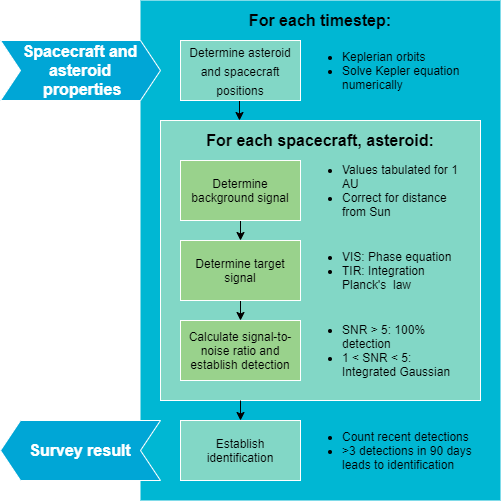
\includegraphics[width=0.7\textwidth]{img/simulation_overview.png}
 \caption{Overview of the simulation architecture and main loops.}
 \label{fig:simulation_overview}
\end{figure}

Currently, no model is publicly available for modelling multi-spacecraft surveys. Therefore, a simulation will be developed. During and after development, the model is also extensively verified and validated. The process for this is described in REF??. Other research (e.g. \cite{Flyeye}, \cite{2017NEOSDT}) has demonstrated the potential for explicitly modelling out the entire survey as it would be conducted by the actual system. This consists of first generating a representative population of asteroids (described in \autoref{sec:modelling_population}), then, at each timestep, calculating the background and target signal (\autoref{sec:modelling_background} and \autoref{sec:modelling_target}, respectively). Knowing these signals, the signal-to-noise ratios can then be determined after estimation of some of the detector properties (\autoref{sec:modelling_hardware_SNR}). The frequency and location of the observations is determined by the search strategy, and resulting cadence (detailed in \autoref{sec:modelling_cadence}) and lastly through repeat observations, it can be determined whether the system is capable of identifying a target (\autoref{sec:modelling_identification}).\\


The architecture of the simulation is shown in \autoref{fig:simulation_overview}. On the top left, the main input parameters to the model are displayed. These are primarily the spacecraft and asteroid properties. Both of these consist of a full set of Keplerian orbital elements per spacecraft or asteroid. The asteroid properties furthermore include the albedo, size, and absolute magnitude of each asteroid; the spacecraft properties include which type of payload the spacecraft is carrying. \\

The simulation consists of a nested loop. Firstly, at the start of each timestep (the time between the timesteps is determined by the survey cadence), the positions of all asteroids and spacecraft are determined by propagation of their orbital elements. Then, in the inside loop, each spacecraft is checked against each asteroid to see if it can detect said asteroid. This is done through calculation of the signal-to-noise ratio (SNR). Lastly, as it is known which asteroids got succesfully detected by which spacecraft, it can be determined if asteroids have been identified. Then, at the end of the simulation, the result is a list of the asteroid population in addition to whether they have been detected, and if so, when. Of course, this data can be further processed.

\section{Population of Asteroids}
\label{sec:modelling_population}
The first component of the simulation is the asteroid population model. This population was already briefly described in \autoref{sec:introduction_NEA}. In this section, more details on the generation of the population and the process of determining the positions of the NEA's, are given. As already mentioned in \autoref{sec:introduction_NEA}, the most comprehensive debiased population model is the one by \cite{PopulationGranvik}. This population model was generated by propagating an intiial population of NEA's based on several known interactions (e.g. gravitational interaction with the planets), and then comparing the resulting population to the results of the NEOWISE mission. Essentially, the problem then reduces to the question: ``What initial population would result in the results that are observed in the NEOWISE mission?''. Then, the initial population model can be fitted to the results of the NEOWISE mission, and an accurate population model is obtained. \\

Of course, this results in a full population of NEA's; whereas a population of \textit{unidentified} NEA's is required for this work. Therefore, a correction to the population was made based on the work of \cite{PopulationHarris}. To do this, the population as given by \cite{PopulationGranvik} was separated, based on absolute magnitude, into bins of width 0.5. Then, it was assumed that the detection of NEAs is roughly uniform over the orbital parameters. The completeness statistics of \cite{PopulationHarris} can then be used to discard a part of the population as \textit{identified}. For example, given 10000 asteroids in the bin width XXYYZZ, where 70\% is considered identified at this time, 7000 asteroids are selected at random and discarded. Of course, the assumption of uniformity in the detection of NEA's is false: highly eccentric NEA's, NEA's that are very dark, or NEA's with a high semi-major axis are more likely to be undetected. However, no data is available on this matter, and therefore no better alternative was deemed to be available. As all simulations will be affected equally, the error is judged to be sufficiently small for practical purposes.

\section{Background Signal}
\label{sec:modelling_background}

\section{Target Signal}
\label{sec:modelling_target}

\section{Hardware Properties and Signal-to-Noise Ratio}
\label{sec:modelling_hardware_SNR}

\section{Search Strategy and Cadence}
\label{sec:modelling_cadence}

\section{Detection and Identification}
\label{sec:modelling_identification}

\newpage
\chapter{Experimental Methodology}

\section{Simulation Overview}

\section{Implementation}

\section{Optimization Methods}

\section{Experimental Process}

\newpage
\chapter{Results and Discussion}
The research process resulted in numerous interesting findings, with implications both for understanding the behavior of the system, as well as for future design efforts considering multi-spacecraft surveys. These results will be presented and discussed in this chapter. Firstly, the effect of increasing or decreasing the number of spacecraft is discussed in \autoref{sec:results_number}. Then, possible payload compositions are assessed in \autoref{sec:results_payload}. Afterwards, the system's orbital elements, and how these are affected by the composition of the system, will be given discourse in \autoref{sec:results_orbits_one} and \autoref{sec:results_orbits_two} for spacecraft in identicial and differing trajectories, respectively. To aid in the interpretation of these results, a possible explanation for the underlying principle is presented in \autoref{sec:results_explanation}. Finishing the discussion, in \autoref{sec:results_performance}, predictions will be made with respect to the performance of an optimal multi-spacecraft survey system, and the impact on future design efforts will be discussed.

\section{Number of Spacecraft}
\label{sec:results_number}

\begin{figure}[htbp]
 \centering
 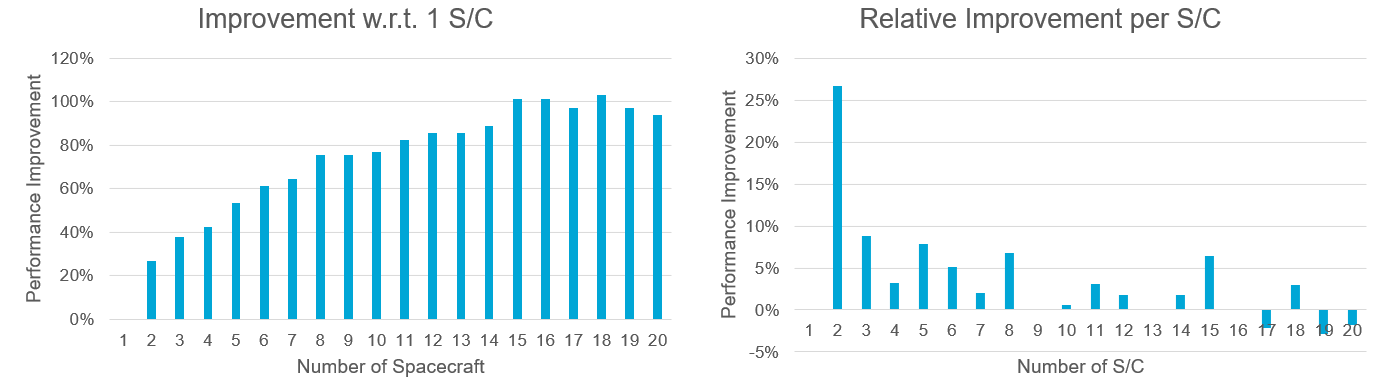
\includegraphics[width=1.0\textwidth]{img/number_sc_vis.png}
 \caption{Improvement in survey completeness gained by increasing the number of spacecraft in a purely visual light wavelength system. The left graph shows the improvement of an $n$-spacecraft system with respect to a system of a single spacecraft, the right graph shows the improvement of an $n$-spacecraft system with respect to an $n-1$-spacecraft system.}
 \label{fig:results_number_vis}
\end{figure}


\begin{figure}[htbp]
 \centering
 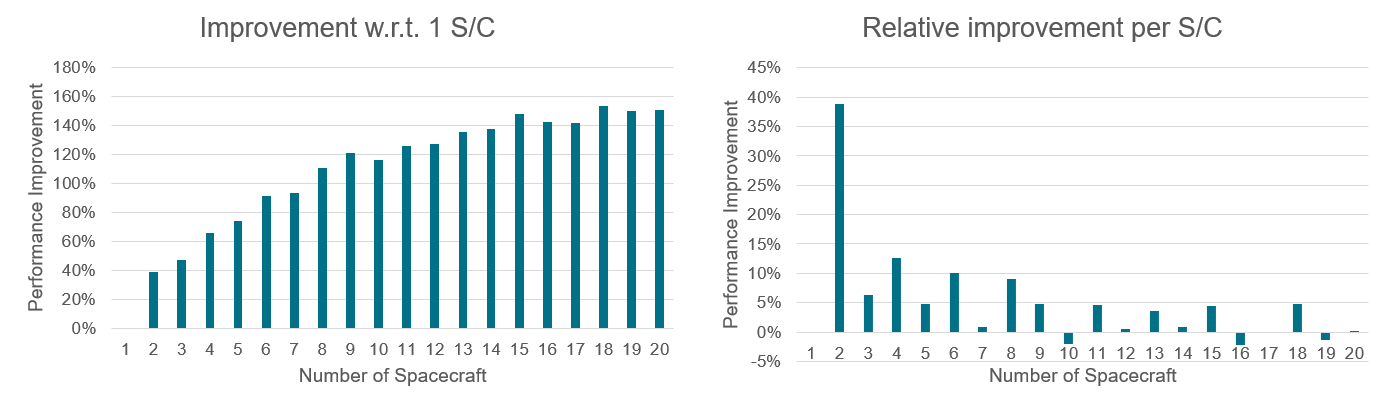
\includegraphics[width=1.0\textwidth]{img/number_sc_tir.png}
 \caption{Improvement in survey completeness gained by increasing the number of spacecraft in a purely thermal infrared wavelength system. The left graph shows the improvement of an $n$-spacecraft system with respect to a system of a single spacecraft, the right graph shows the improvement of an $n$-spacecraft system with respect to an $n-1$-spacecraft system.}
 \label{fig:results_number_tir}
\end{figure}

As explained previously, the number of spacecraft in the system is a parameter that does not have an optimum with respect to the obtained survey completeness: adding additional spacecraft will logically never degrade the performance of the system. However, in practice other constraints (primarily economical) will be present. Therefore, the increase in performance resulting from such an increased investment is of particular interest. \autoref{fig:results_number_vis} and \autoref{fig:results_number_tir} show the performance increase obtained as a function of the number of spacecraft, for the visual spectrum and thermal infrared, respectively. Several observations can be made, which will be listed and subsequently discussed below.\\

Firstly, significant diminishing returns present themselves for both spectra; the additional value of an extra spacecraft decreases exponentially with the number of spacecraft already present in the system. Performance increases gained per additional spacecraft fall to around 5\% when surpassing 5 spacecraft in the system. Beyond 10 spacecraft, the increases start to fall below the variance in the results, leading to the appearance that addition of spacecraft would yield a decrease in performance, which is logically not the case. This means that, although large initial improvements in performance can be gained from utilizing a multi-spacecraft system, simply increasing the number of survey spacecraft can not bring us arbitrarily close to 100\% survey completeness; when increasing beyond approximately 5 spacecraft, it is recommended to focus efforts on improving other areas of the system for the mission to remain efficient. \\

This fact compounds the second finding: even the most efficient addition - adding a second spacecraft to a single spacecraft survey system - does not come close to increasing the system performance by 100\%. In other words: increasing the number of spacecraft will \textit{decrease} the number of asteroids detected \textit{per spacecraft}. While this finding might seem irrelevant from a mission design point-of-view, as the overall performance still increases, it is nevertheless important to consider in the context of other mission constraints, such as budget. \\

The third result is that thermal infrared systems feature a larger relative improvement to survey performance as the number of spacecraft increases, i.e. thermal infrared systems benefit more from additional spacecraft. This trend continues for higher numbers of spacecraft, with thermal infrared systems reaching a 100\% improvement around 7-8 spacecraft, compared to visual light systems requiring 15-16 spacecraft to achieve a similar performance gain. This, combined with the fact that thermal infrared systems have been shown to be the best choice for future NEA missions (see e.g. \cite{2017NEOSDT}, \cite{ThesisOlga}), suggests a multi-spacecraft system should also comprise thermal infrared telescopes. This will be investigated in more detail in \autoref{sec:results_payload}.\\

Finally, it is evident that a variance of around 1-2\% is present in the survey performance results, relative to a smooth exponentially decreasing curve. It was found that this variance is also present when repeatedly sampling the simulation using the same input parameters. Therfore, in these and subsequent results, it will be assumed that this is simply a result of the stochasticity in the model. Possible other explanations will be ruled out further in REFF.

\section{Payload}
\label{sec:results_payload}
\begin{figure}[htbp]
 \centering
 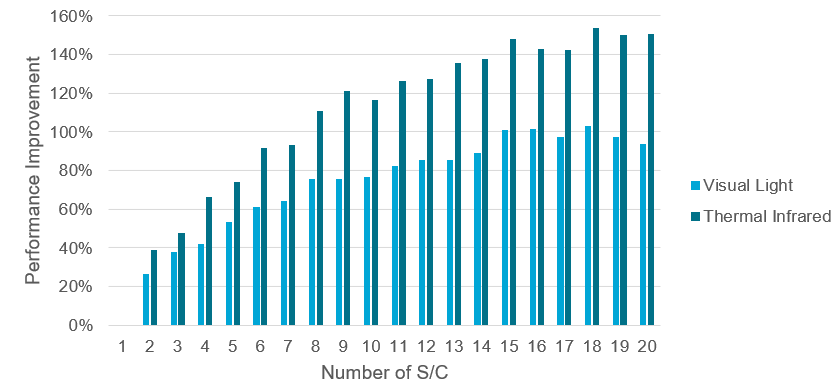
\includegraphics[width=0.7\textwidth]{img/tir_vs_vis_many.png}
 \caption{Comparison of relative increase in performance gained relative to a single spacecraft system for visual and thermal infrared systems.}
 \label{fig:tir_vs_vis_many}
\end{figure}

\begin{figure}[htbp]
 \centering
 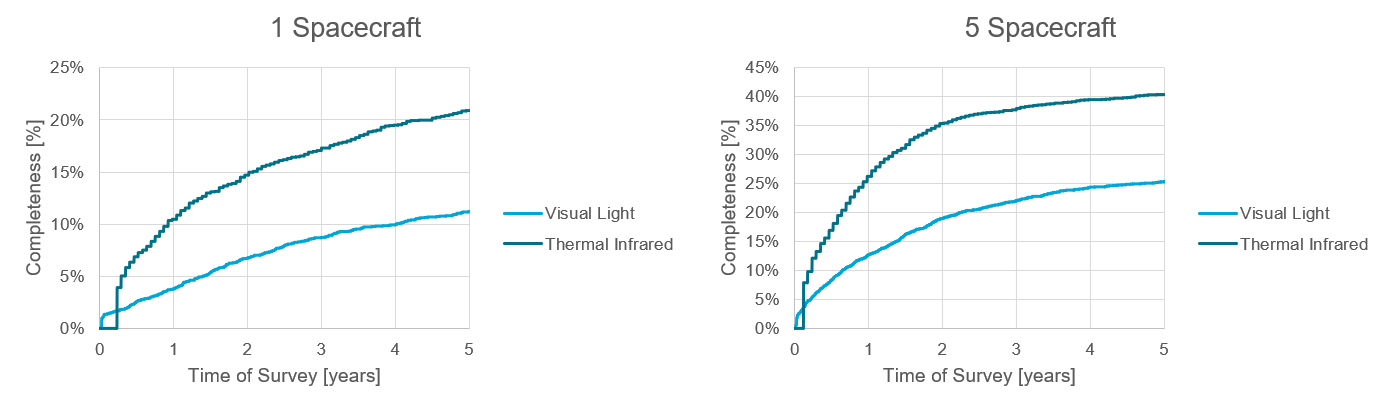
\includegraphics[width=1.0\textwidth]{img/tir_vs_vis_1_5.png}
 \caption{Progress of survey completeness over a five year survey for a 1-spacecraft and 5-spacecraft system, comparing visual light and thermal infrared.}
 \label{fig:tir_vs_vis_nohybrid}
\end{figure}


As mentioned in the previous section, initial result suggest thermal infrared systems to be the optimal choice for multi-spacecraft systems because of their predicted higher performance in single-spacecraft systems, and higher benefit from increasing the number of spacecraft. The latter effect is shown in \autoref{fig:tir_vs_vis_many}. In this section, the payload composition will be investigated in more detail. Particular interest is placed in the effect of survey length - as visual light systems feature a faster cadence - and in possible synergistic effects in systems featuring both visual light and thermal infrared telescopes. When interpreting the results of this chapter, it is important to keep in mind the fact that these simulations were carried out assuming contemporary hardware. Advances in either type of telescope or sensor might warrant a future reassessment.\\

Firstly, the performances for systems featuring only one payload type were modelled. For comparison, this analysis was carried out for a 1-spacecraft and a 5-spacecraft system. Because, as shown in the previous section, the payload types exhibit similar behavior when the number of spacecraft is altered, this was assumed to be representative of other numbers of spacecraft as well. The resulting survey performance as a function of time can be seen in \autoref{fig:tir_vs_vis_nohybrid}. Note that, contrary to previous figures, these graphs show the \textit{absolute} survey completeness, not the completeness relative to a benchmark. In the results, it can be observed that initially, the visual light system features a higher completeness due to its faster cadence. However, the thermal infrared system quickly surpasses it as time progresses. This means that the faster cadence granted by the lower integration times and larger sensor sizes of the visual light system does not weight up to the increased sensitivity of the thermal infrared system on the timescales of survey missions; not only is the final survey completeness more than 10\% higher for a thermal infrared system, it also manages to achieve the same performance as a 5-year visual light survey in only a single year in both examined cases. This agrees with the findings of \cite{ThesisOlga} that for systems where quick detections are important, such as impact last-warning, thermal infrared is also a superior option. \\

\begin{figure}[htbp]
 \centering
 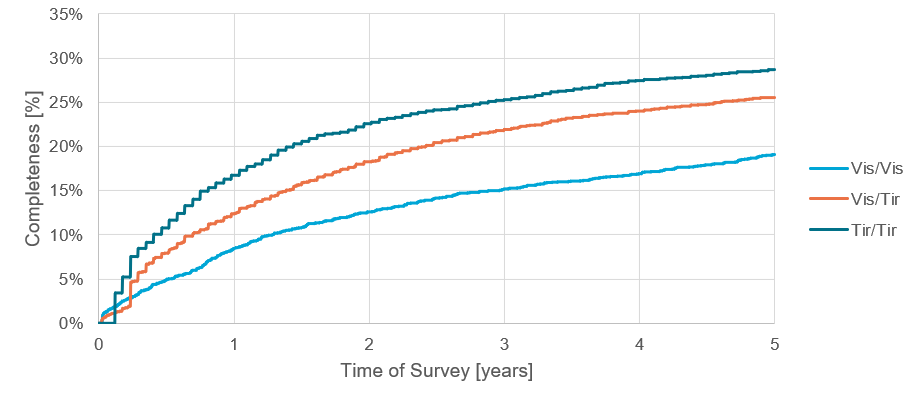
\includegraphics[width=0.8\textwidth]{img/tir_vs_vis_2_hybrid.png}
 \caption{Progress of survey completeness over a five year survey for all possible payload combinations in a 2-spacecraft system.}
 \label{fig:payload_hybrid_one}
\end{figure}

\begin{figure}[htbp]
 \centering
 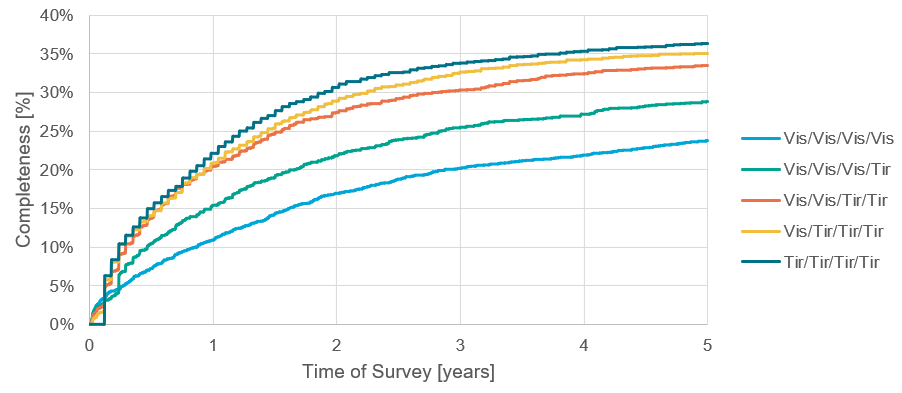
\includegraphics[width=0.8\textwidth]{img/tir_vs_vis_4_hybrid.png}
 \caption{Progress of survey completeness over a five year survey for all possible payload combinations in a 4-spacecraft system.}
 \label{fig:payload_hybrid_two}
\end{figure}

In continuation of the payload analysis, systems utilizing a combination of visual light and thermal infrared telescopes were examined. The reasoning is that the higher sensitivity of thermal infrared systems combined with the higher cadence of visual light systems might result in a synergistic effect where fast, hard to detect NEA's can still be identified successfully. However, as can be seen from the results for 2- and 4-spacecraft systems in \autoref{fig:payload_hybrid_one} and \autoref{fig:payload_hybrid_two}, respectively, this is not the case. A system comprising purely infrared telescopes yields the best results, and performance increases progressively as the number of thermal infrared telescopes in the system increases. This means that in general thermal infrared is the preferred payload type for deep space multi-spacecraft systems. Note however that this assertion is made under the assumption of a ``dumb'' search strategy, where the system simply repeatedly images the entire sky. Possible applications of fast visual light telescopes as ``follow-up'' telescopes - as demonstrated by the Catalina Sky Survey - might still be a feasible option, although this would first require research into such advanced search strategies.

\section{Orbital Elements I: Co-orbital Spacecraft}
\label{sec:results_orbits_one}
Next, the orbital elements of the system are inspected. This is done both to find what the effect is of the orbital elements on the performance, but also how the payload and number of spacecraft affect the optimal orbital elements of the system. To facilitate analysis, and to later judge the results of the optimizer more accurately, the orbits are first analysed for a system of co-orbital spacecraft. That is, all orbital elements, except for the anomaly at epoch, are the same for all spacecraft. In addition, the separation in anomalies of the spacecraft is the same for all spacecraft. This was done to vastly reduce the parameter space, and to reduce accidental overfitting to the population model. The latter follows from the fact that, logically, only the angular distance between the spacecraft should influence the result, not the absolute starting position, as the NEA's are distributed in a radially symmetrical fashion. I.e., a system with two spacecraft at mean anomaly at epoch $0$ and $\pi$ should give the same result as starting at $\pi/2$ and $3\pi/2$, only the inter-spacecraft distance is relevant.\\

\subsection{Semi-major axis}

\begin{figure}[htbp]
 \centering
 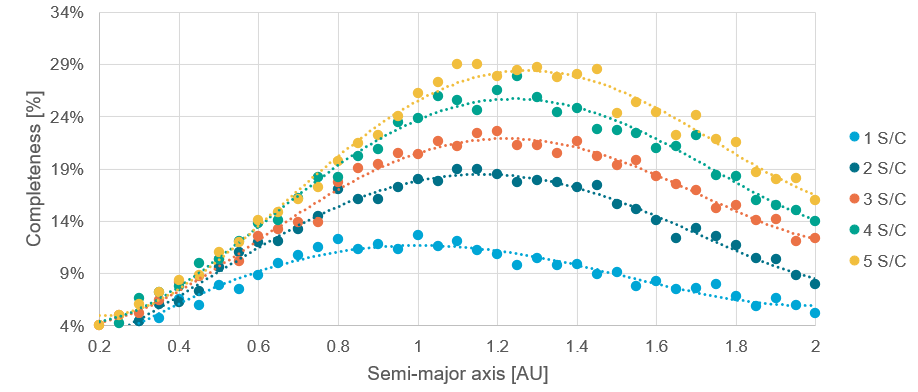
\includegraphics[width=0.8\textwidth]{img/vis_semi_maj.png}
 \caption{Visual light survey performance as a function of semi-major axis for 1 to 5 spacecraft.}
 \label{fig:vis_semi_maj}
\end{figure}

\begin{figure}[htbp]
 \centering
 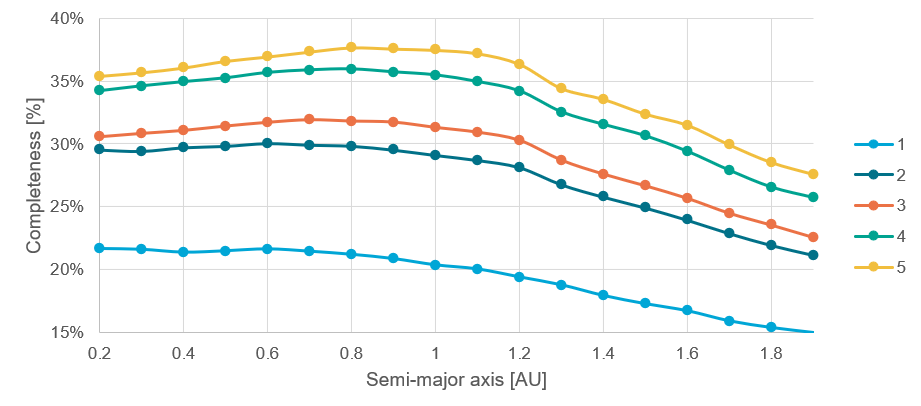
\includegraphics[width=0.8\textwidth]{img/tir_semi_maj.png}
 \caption{Thermal infrared survey performance as a function of semi-major axis for 1 to 5 spacecraft.}
 \label{fig:tir_semi_maj}
\end{figure}

In \autoref{fig:vis_semi_maj}, the expected survey performance as a function of semi-major axis is shown for visual light systems, and in \autoref{fig:tir_semi_maj} for thermal infrared systems. Contrary to the number of spacecraft, it is clear that the semi-major axis has an optimal value. In addition, the region surrounding the optimum is very flat. Thus, locally, the solution is not sensitive to changes in semi-major axis up to a distance of approximately $0.1~\mathrm{AU}$ from the optimum. Two important conclusions are drawn here: Firstly, a wide range of semi-major axes lead to a well performing system. Secondly, due to the variance in results discussed earlier, it is difficult to pinpoint an exact optimal value. Therefore, in mission design, other considerations can and should be prioritized to determine a more precise semi-major axis. \\

The second factor of note is the change in the optimal semi-major axis as the number of spacecraft increases. It can be observed that for visual light systems, the optimal semi-major axis is essentially unchanging for $n \leq 5$. However, for thermal infrared systems, there is clearly an increase in optimal semi-major axis as $n$ increases. This is further illustrated in \autoref{fig:semi_maj_function_of_n}, where the optimal semi-major axis is given as a function of the number of spacecraft explicitly. Here, it can be observed that the optimizer indeed has difficulty pinpointing the exact optimum, but instead finishes on a value somewhere in the optimal range. In addition, the semi-major axis becomes larger for higher numbers of spacecraft for thermal infrared systems. For visual light systems at higher numbers of spacecraft this also starts to occur. An explanation for this phenomenon is proposed in \autoref{sec:results_explanation}.

TO DO: Getallen noemen.

\begin{figure}[htbp]
 \centering
 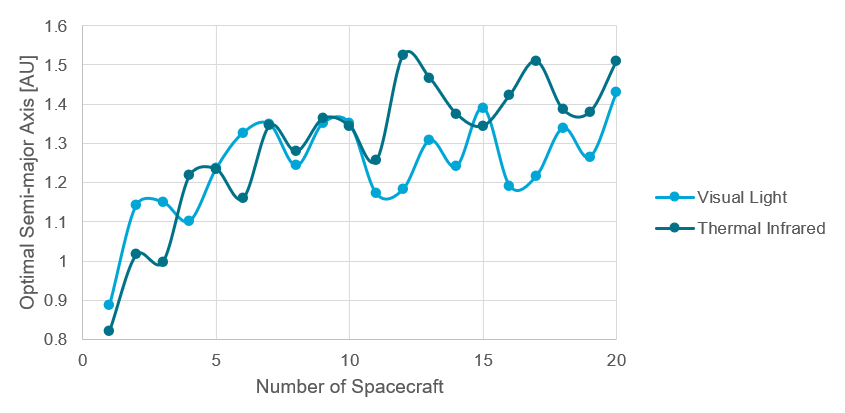
\includegraphics[width=0.8\textwidth]{img/semi_maj_function_of_n.png}
 \caption{Optimal semi-major axis as a function of the number of spacecraft in the system.}
 \label{fig:semi_maj_function_of_n}
\end{figure}



\subsection{Eccentricity}
\begin{figure}[htbp]
 \centering
 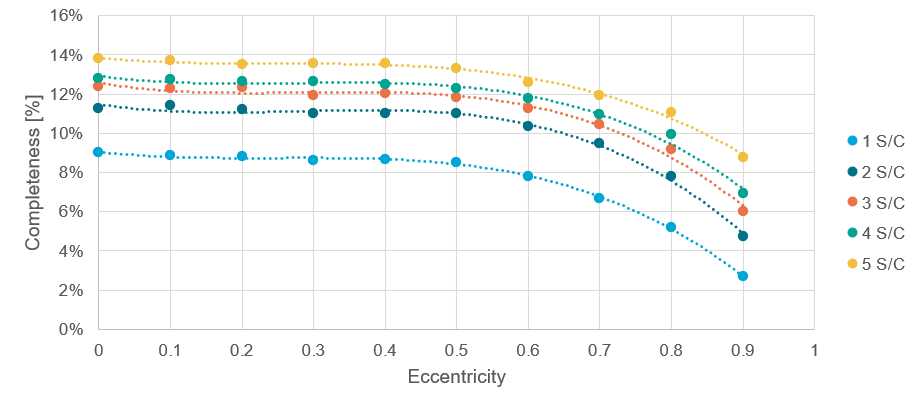
\includegraphics[width=0.8\textwidth]{img/vis_ecc.png}
 \caption{Visual light survey performance as a function of eccentricity for 1 to 5 spacecraft.}
 \label{fig:vis_ecc}
\end{figure}

\begin{figure}[htbp]
 \centering
 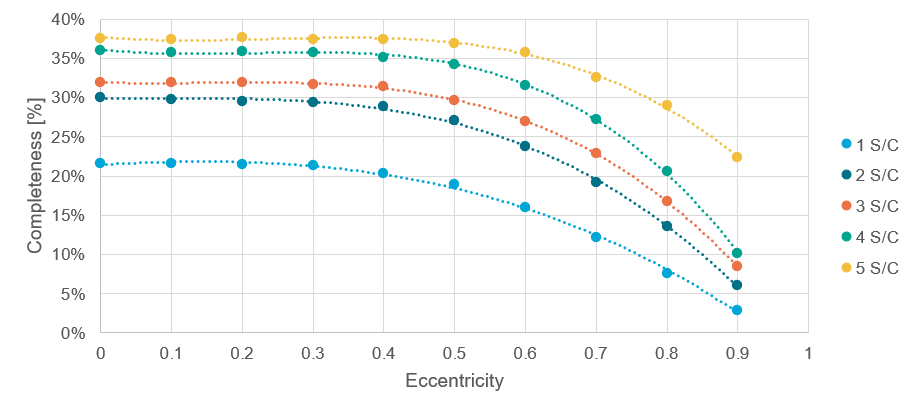
\includegraphics[width=0.8\textwidth]{img/tir_ecc.png}
 \caption{Thermal infrared survey performance as a function of eccentricity for 1 to 5 spacecraft.}
 \label{fig:tir_ecc}
\end{figure}

Results with regards to varying the eccentricity are shown in \autoref{fig:vis_ecc} for visual light systems and \autoref{fig:tir_ecc} for thermal infrared systems. It is readily apparent that for both systems, a circular orbit is preferred. It is hypothesized that this is the case because eccentricity causes the system to deviate from the optimal semi-major axis found in the previous subsection. This is further supported by the empirical finding that the optimal semi-major axis at a given eccentricity results in an apohelion distance roughly equal to the optimal semi-major axis at 0 eccentricity. That is:
\begin{equation}
 a_{opt}(e) \approx \frac{a_{opt}(0)}{1+e}
\end{equation}
This is further illustrated in \autoref{fig:eccentricity_optimal}. This result is theorized to occur because the spacecraft will, in this solution, still spend a large portion of its orbit in the optimal semi-major axis range. However, not enough data are available to ascertain statistical significance for this finding.

\begin{figure}[htbp]
 \centering
 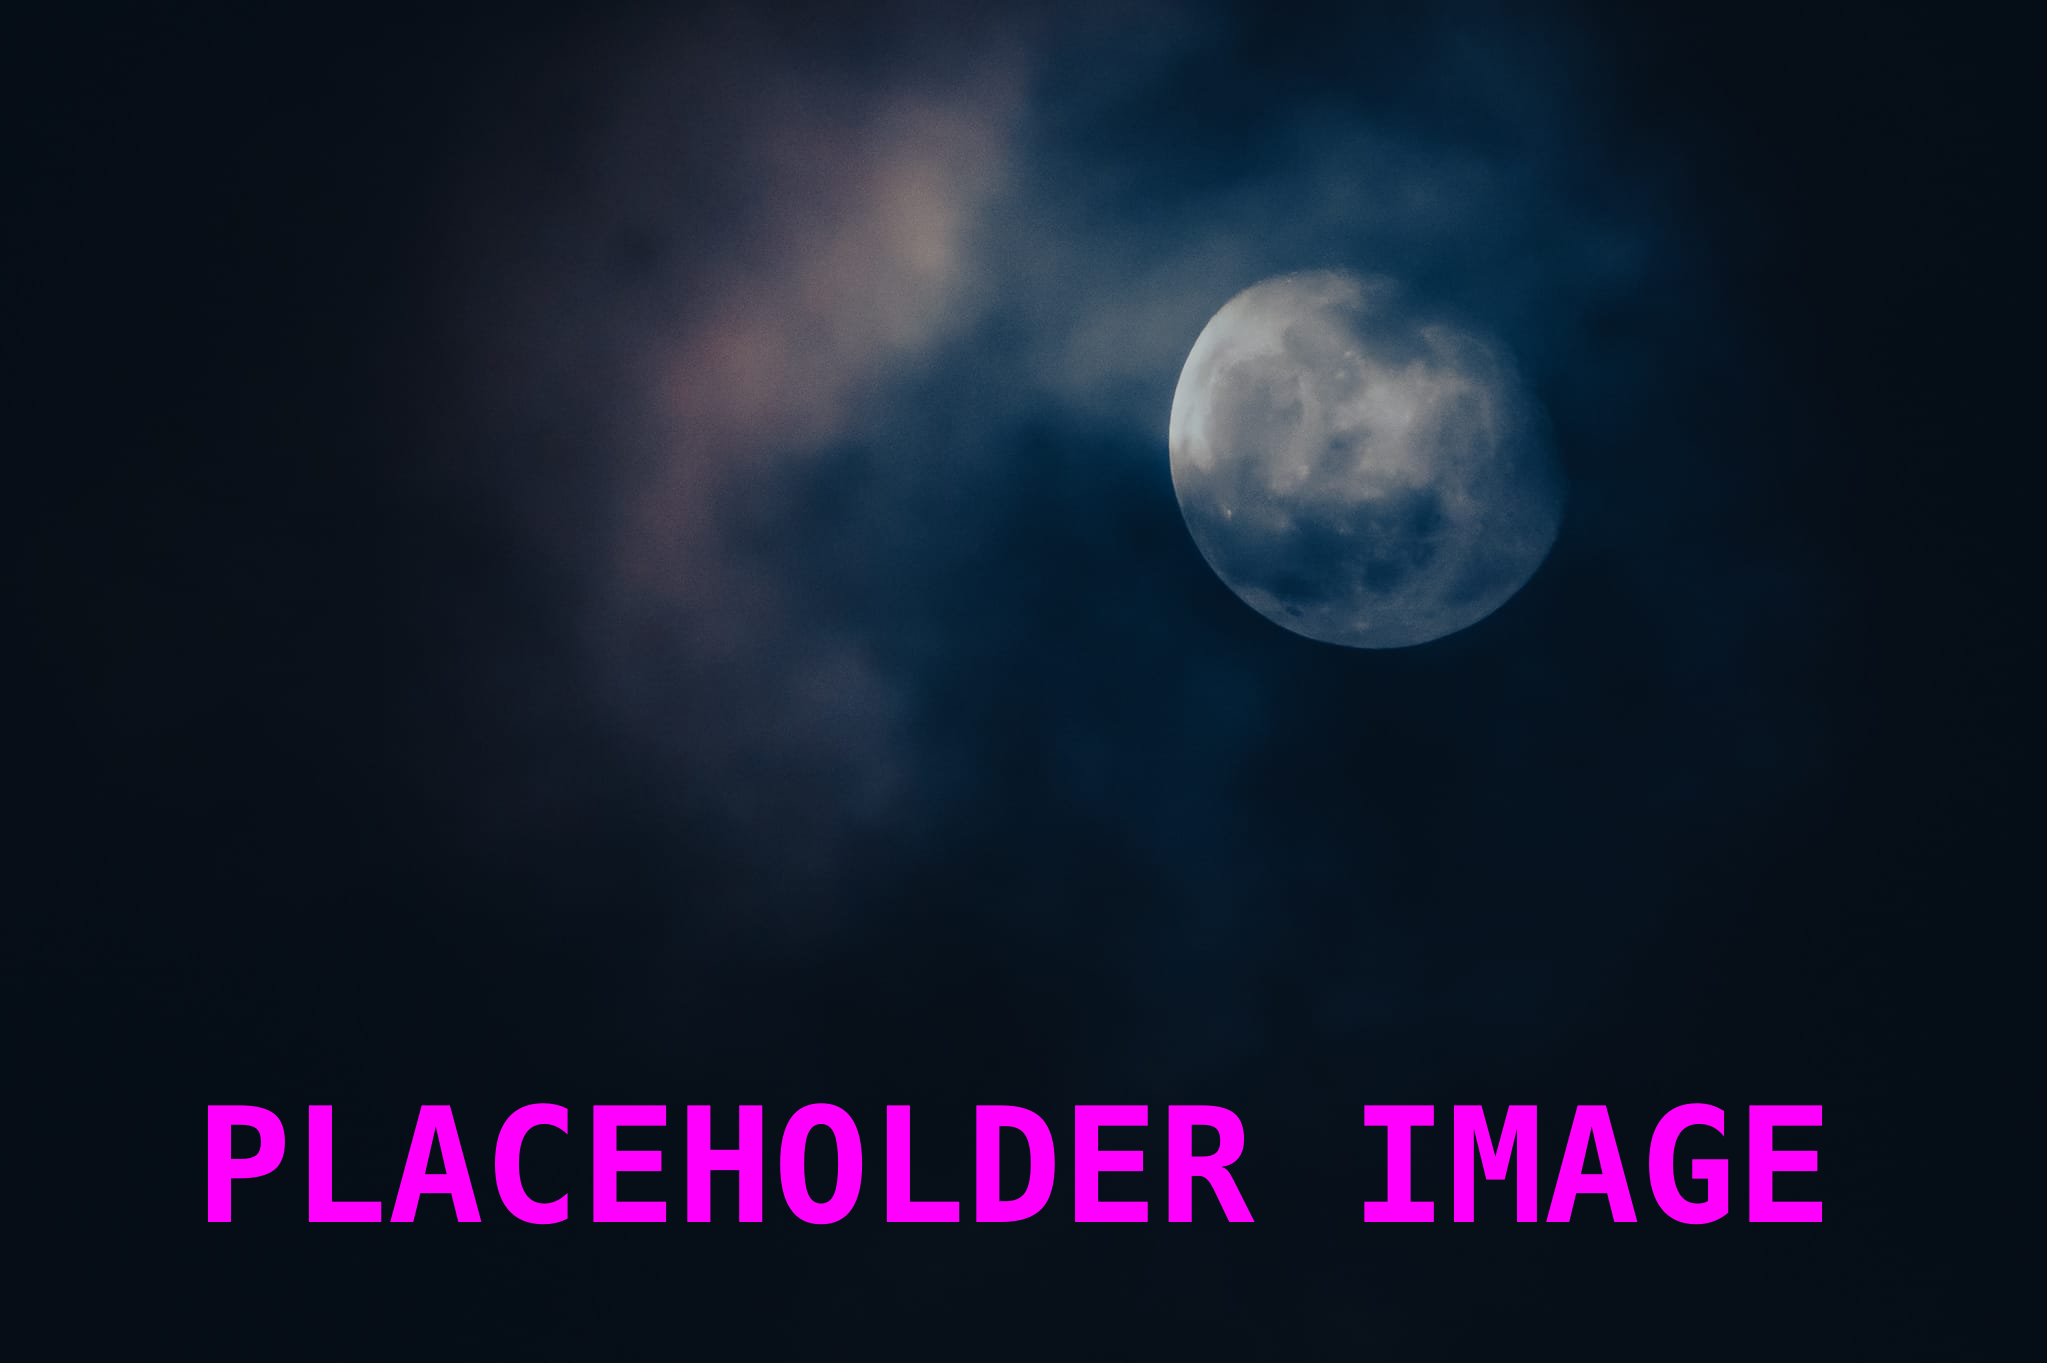
\includegraphics[width=1.0\textwidth]{img/eccentricity_optimal.png}
 \caption{Relationship between optimal semi-major axis, eccentricity, and the resulting perihelion for 1-5 spacecraft.}
 \label{fig:eccentricity_optimal}
\end{figure}


\subsection{Mean Anomaly at Epoch}
\begin{figure}
 \centering
 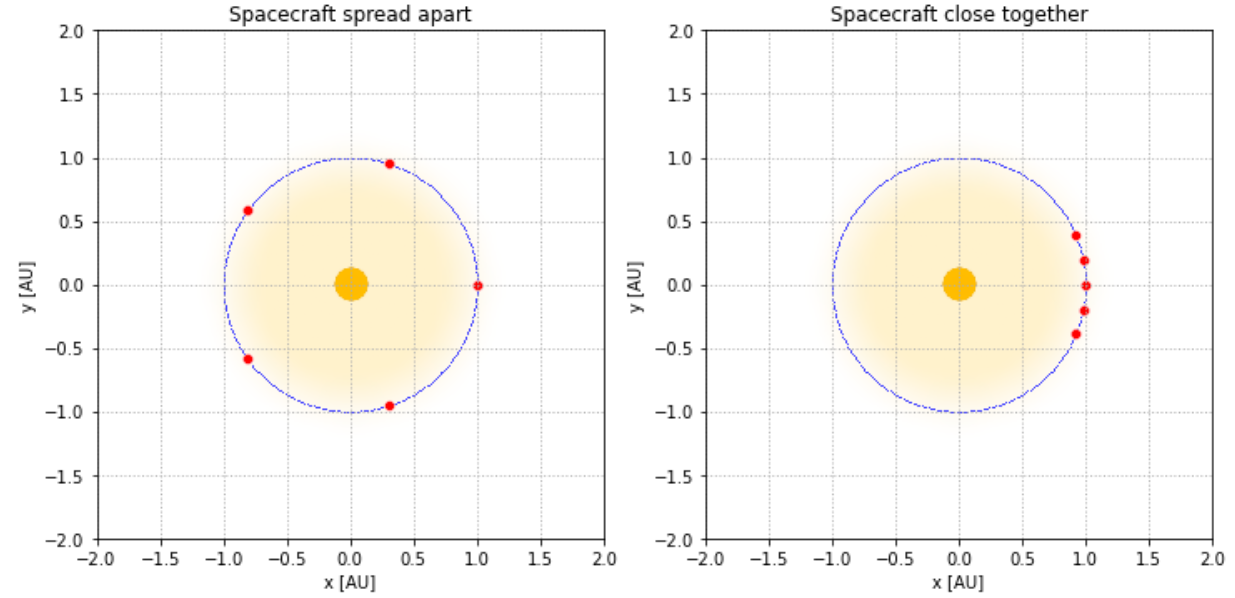
\includegraphics[width=1.0\textwidth]{img/spread_illustration.png}
 \caption{Illustration of a high ($2\pi/5~\mathrm{rad}$ and a low ($0.3~\mathrm{rad}$) inter-spacecraft distance.}
 \label{fig:spread_illustration}
\end{figure}

The last parameter to be considered for the co-orbital solutions is the mean anomaly at epoch. As previously explained, the mean anomaly will not be considered for each spacecraft separately. Instead, the concept of inter-spacecraft spread is introduced. This inter-spacecraft spread is simply defined as the difference in anomaly at epoch of one spacecraft to the next, in such a way that the formation is centered around $\theta=0$. This means that, with inter-spacecraft spread $\Delta \theta$, the mean anomaly at epoch $\theta$ of spacecraft $n$ in a system of $N$ spacecraft is:
\begin{equation}
 \theta_n = (n-1) \cdot \Delta \theta - \frac{N-1}{2}\Delta \theta
\end{equation}
This equation and the resulting formation is shown in \autoref{fig:spread_illustration}. A lower boundary of 0.3 rad was chosen to ensure triangulation would remain possible. In addition, to maintain the separation between all spacecraft, the full formation can not span more than $2\pi$ rad. This results in the boundaries $0.3 \leq \Delta \theta \leq 2\pi/N$. The hypothesized effect of changing the spread is composed of two effects: On the one hand, spreading out the spacecraft more allows for viewing a larger portion of the sky simultaneously, and reduces blind spots, as explained in REFFF. On the other hand, as spacecraft are closer together, the chances of obtaining a simultaneous detection of the same asteroid - and thereby achieving triangulation - is increased, thereby leading to a faster detection.\\

\begin{figure}[htbp]
 \centering
 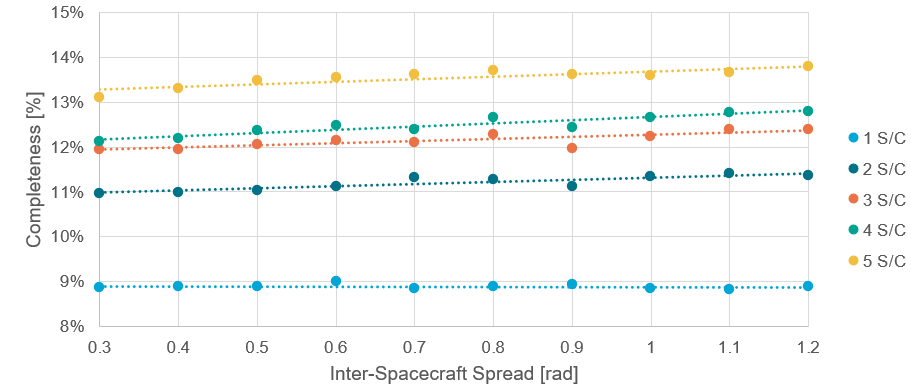
\includegraphics[width=0.8\textwidth]{img/vis_spread.png}
 \caption{Visual light survey performance as a function of angular separation between spacecraft for 1 to 5 spacecraft.}
 \label{fig:vis_spread}
\end{figure}

\begin{figure}[htbp]
 \centering
 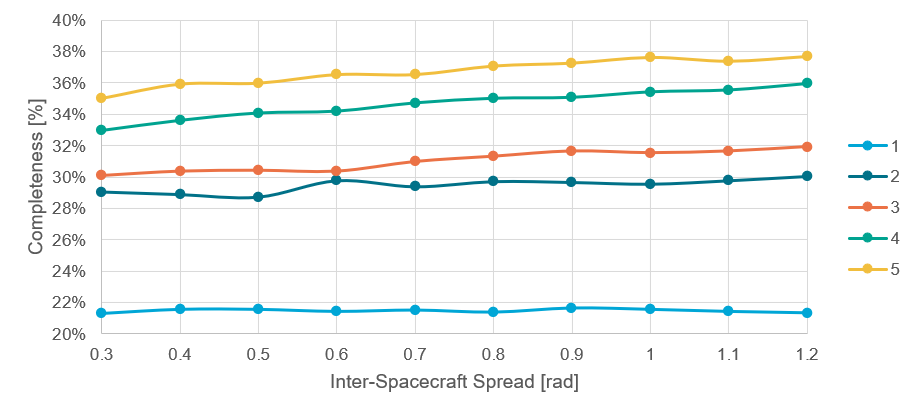
\includegraphics[width=0.8\textwidth]{img/tir_spread.png}
 \caption{Thermal infrared survey performance as a function of angular separation between spacecraft for 1 to 5 spacecraft.}
 \label{fig:tir_spread}
\end{figure}

Results for visual light and thermal infrared are shown in \autoref{fig:vis_spread} and \autoref{fig:tir_spread}, respectively. It is observed that an increase in the angular distance between the spacecraft will increase the performance of the system. Therefore, the effect of observing a larger part of the sky effectively is stronger than the increased chance at succesful triangulation. Practically, this implies that a multi-spacecraft survey should aim to distribute the spacecraft as much as possible over the orbit, even if e.g. communications requirements do not allow the system to be spread out over the entire orbit.

\section{Orbital Elements II: Non Co-orbital Spacecraft}
\label{sec:results_orbits_two}
A logical continuation of the above analysis would be to investigate systems in which all spacecraft are allowed to have different orbital elements per spacecraft. This complicates the analysis significantly, as the dimensionality of the problem rapidly increases. Therefore, additional special attention has to be paid to the performance of the optimizer, and to run validation tests on its results. In addition, to aid in comparison, three sets of optimization parameters were analysed. Firstly, a system which has all spacecraft spread out as much as possible, in a single circular orbit. From the results in the previous section, it follows that this is the optimal solution. Secondly, a system in which each spacecraft can have a distinct semi-major axis and anomaly at epoch. Because spacecraft with different semi-major axes have different orbital periods, the spacecraft can not be spread out evenly a priori. Therefore, the optimizer has to take care of this task as well, and not just the semi-major axes. Lastly, a similar set of parameters is analysed, but with orbits that are allowed to be non-circular. In that case, the parameter space comprises a semi-major axis, true anomaly at epoch, and eccentricity for each spacecraft.\\

\begin{figure}[htbp]
 \centering
 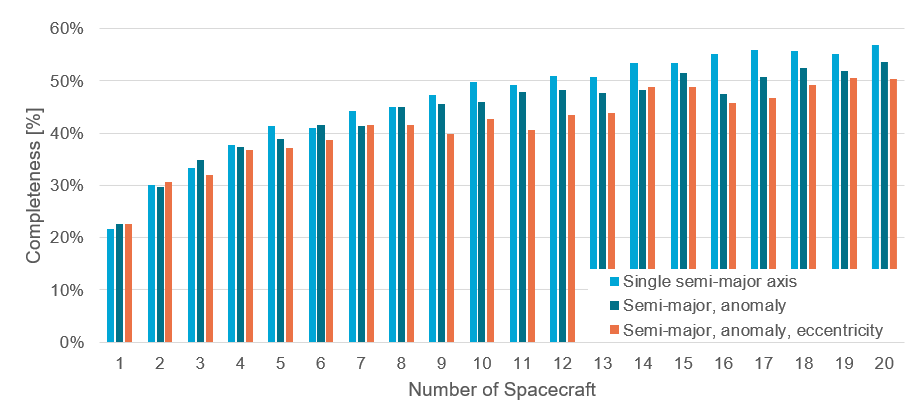
\includegraphics[width=1.0\textwidth]{img/performance_free.png}
 \caption{Performances for systems optimized for either a single semi-major axis, distinct semi-major axes and anomalies per spacecraft, or distinct semi-major axes, anomalies and eccentricities per spacecraft.}
 \label{fig:performance_free}
\end{figure}
The results of the optimization processes can be seen in \autoref{fig:performance_free}. It can be seen that several performance breakpoints are present: for low numbers of spacecraft, approximately $1 \leq n \leq 5$, all three methods result in similar performances. Then, for approximately $6 \leq n \leq 10$, the performance of the optimization including eccentricity starts degrading relative to the other two. Lastly, for $n > 10$, the ``simple'' solution with the spacecraft in the same orbit, spaced equally, is superior to the other two methods. These results might be surprising to some readers: one would expect the performance to either increase, or stay equal, as more parameters become available to the optimizer. After all, all solutions found for a circular, co-orbital system of spacecraft (i.e. only a single semi-major axis gets determined by the optimizer), can be recreated by the other two optimizers, and therefore they can reach the same performance. The source of this discrepancy is twofold. The first aspect is the problem of the optimizer overfitting to the noise in the system. The second aspect is related to the actual performance benefits obtainable through these more complex solutions. Although the results here might seem inconclusive, the combination of both aspects will allow drawing some important conclusions.\\

\begin{figure}[htbp]
 \centering
 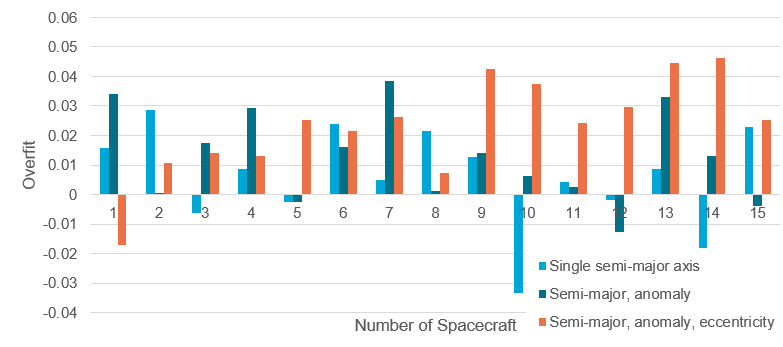
\includegraphics[width=1.0\textwidth]{img/overfit_free.png}
 \caption{Overfit of the optimizer per number of spacecraft.}
 \label{fig:overfit_free}
\end{figure}
\begin{figure}[htbp]
 \centering
 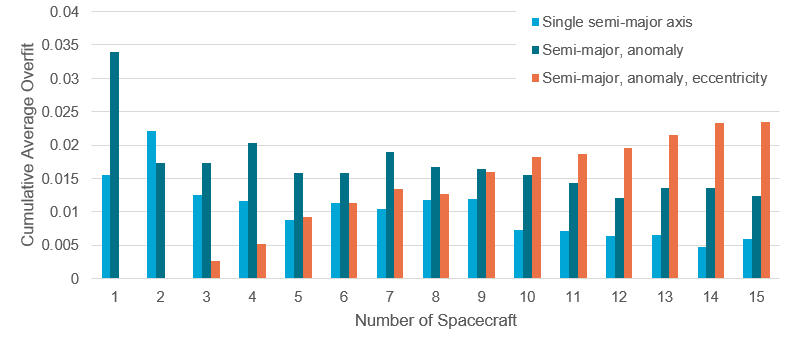
\includegraphics[width=1.0\textwidth]{img/overfit_free_cumulative_average.png}
 \caption{Cumulative average of the overfit of the optimizer per number of spacecraft.}
 \label{fig:overfit_free_cumulative_average}
\end{figure}

First, the problem of overfit will be adressed. To illustrate the occurence of overfit at higher dimensionalities, \autoref{fig:overfit_free} gives the overfit for each optimization problem, per spacecraft. Overfit is defined simply as the difference between the learning performance (i.e. the performance predicted by the optimizer for its solution) and the validation performance (the actual performance which can be expected at the solution). As \autoref{fig:overfit_free} is hard to interpret directly, \autoref{fig:overfit_free_cumulative_average} provides the cumulative average up to and including a certain number of spacecraft. Several observations are made here:
\begin{itemize}
 \item As the number of spacecraft increases, the average overfit of the single semi-major axis system decreases. In other words, for a higher number of spacecraft, the optimizer performs better. This occurs because, in this system, the dimensionality does not increase, and therefore the task of the optimizer is equally hard. However, as the distribution of spacecraft becomes more uniform, the system will overfit less to the population as the importance of the starting position of each spacecraft becomes smaller. In other words, a higher number of spacecraft incurs a regularizing effect on the optimizer.
 \item Secondly, the average overfit for the system with distinct semi-major axis and anomaly, but no eccentricity, per spacecraft, exhibits no statistically significant slope. The degree over overfit levels out around 1-1.5\%. At this degree of overfitting, the optimizer is capable of finding a solution to the problem. 
 \item Lastly, the system optimized for semi-major axis, anomaly and eccentricity, shows an \textit{increase} in overfitting. I.e., the optimizer is not capable of keeping up with the increasing dimensionality of the problem, and the quality of the result continually decreases.
\end{itemize}
Before investigating the second point, first some of the solutions of the optimizer will be examined, along with their training progress. The solutions to be investigated are two, six and eleven spacecraft. The one spacecraft case is omitted as the optimal solution is already known from previous analysis to be the optimal solution to the single semi-major axis system. The six and eleven spacecraft cases were chosen as they represent the first solution after the performance breakpoints discussed earlier.
\begin{figure}[htbp]
 \centering
 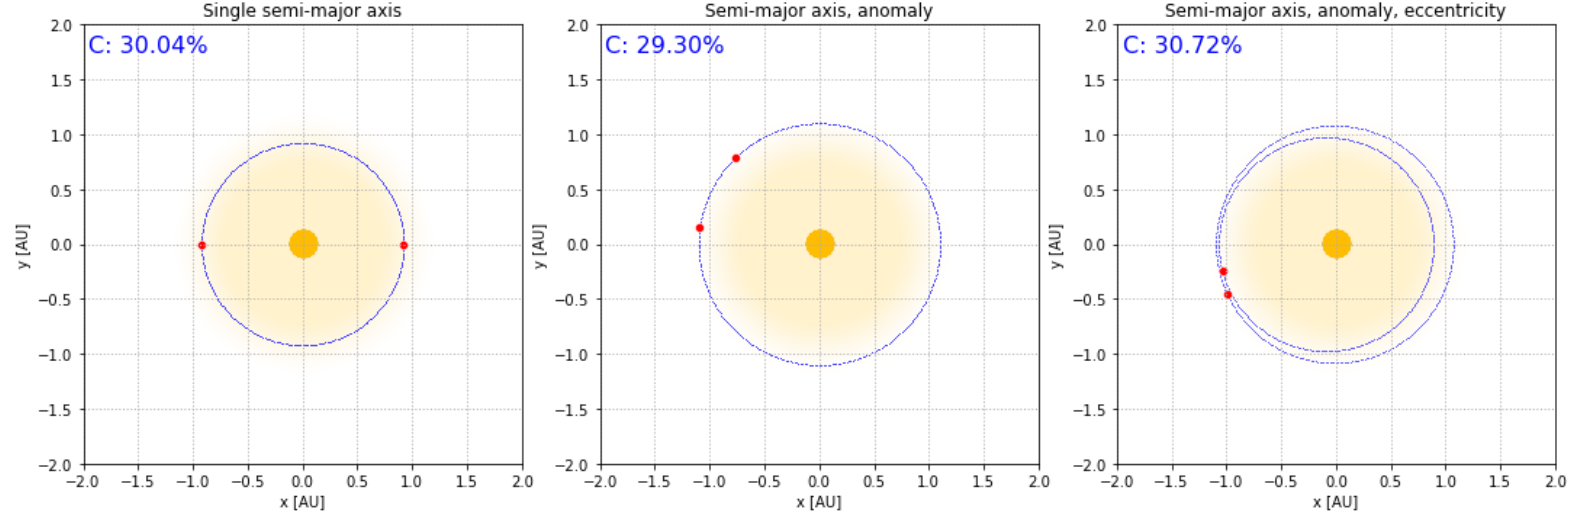
\includegraphics[width=1.0\textwidth]{img/orbits_2.png}
 \caption{Optimization results for systems with two spacecraft.}
 \label{fig:orbits_2}
\end{figure}
\begin{figure}[htbp]
 \centering
 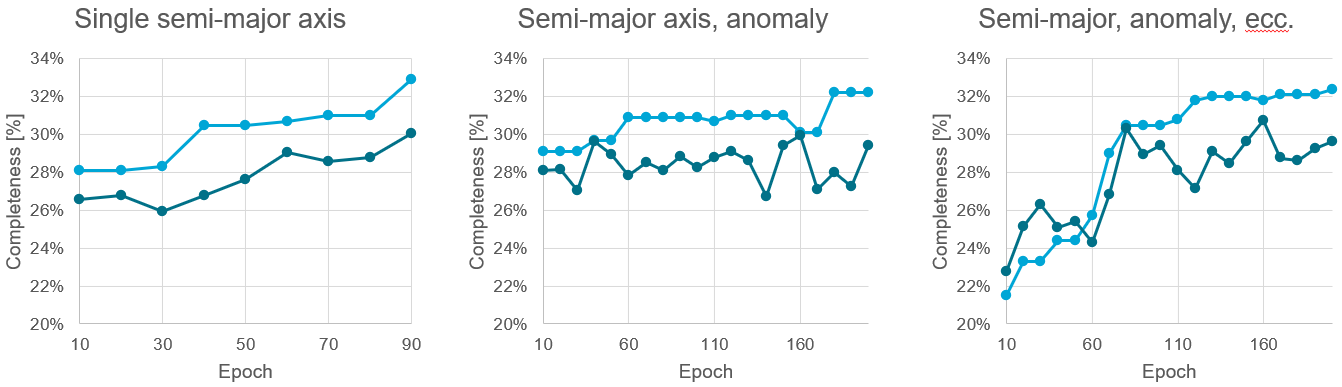
\includegraphics[width=1.0\textwidth]{img/val_orbits_2.png}
 \caption{Learning/validation results for systems with two spacecraft.}
 \label{fig:val_orbits_2}
\end{figure}



\begin{figure}[htbp]
 \centering
 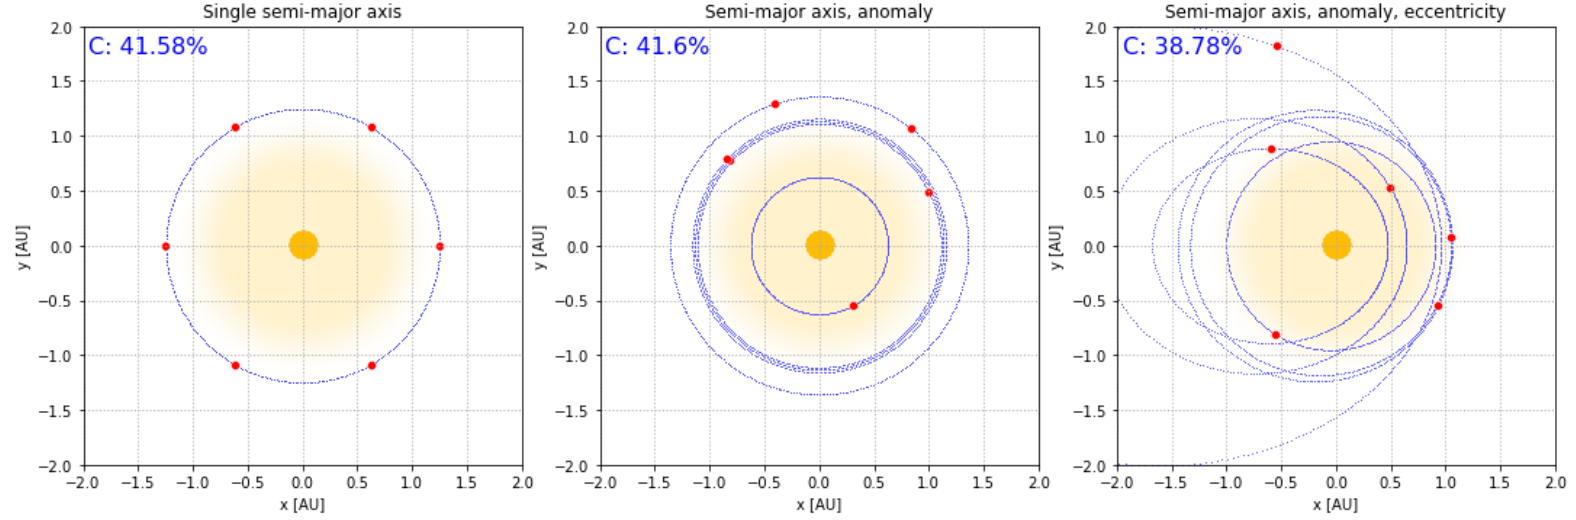
\includegraphics[width=1.0\textwidth]{img/orbits_6.png}
 \caption{Optimization results for systems with six spacecraft.}
 \label{fig:orbits_6}
\end{figure}
\begin{figure}[htbp]
 \centering
 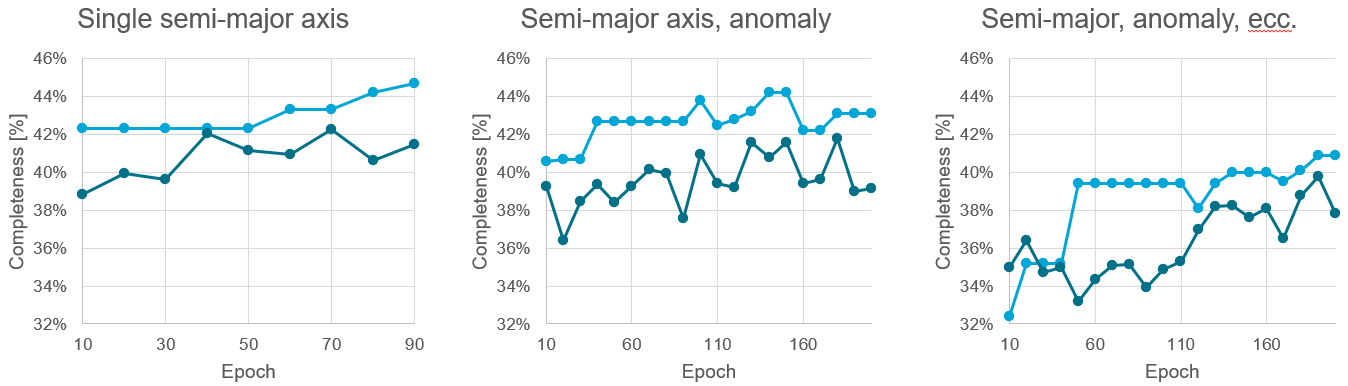
\includegraphics[width=1.0\textwidth]{img/val_orbits_6.png}
 \caption{Learning/validation results for systems with six spacecraft.}
 \label{fig:val_orbits_6}
\end{figure}



\begin{figure}[htbp]
 \centering
 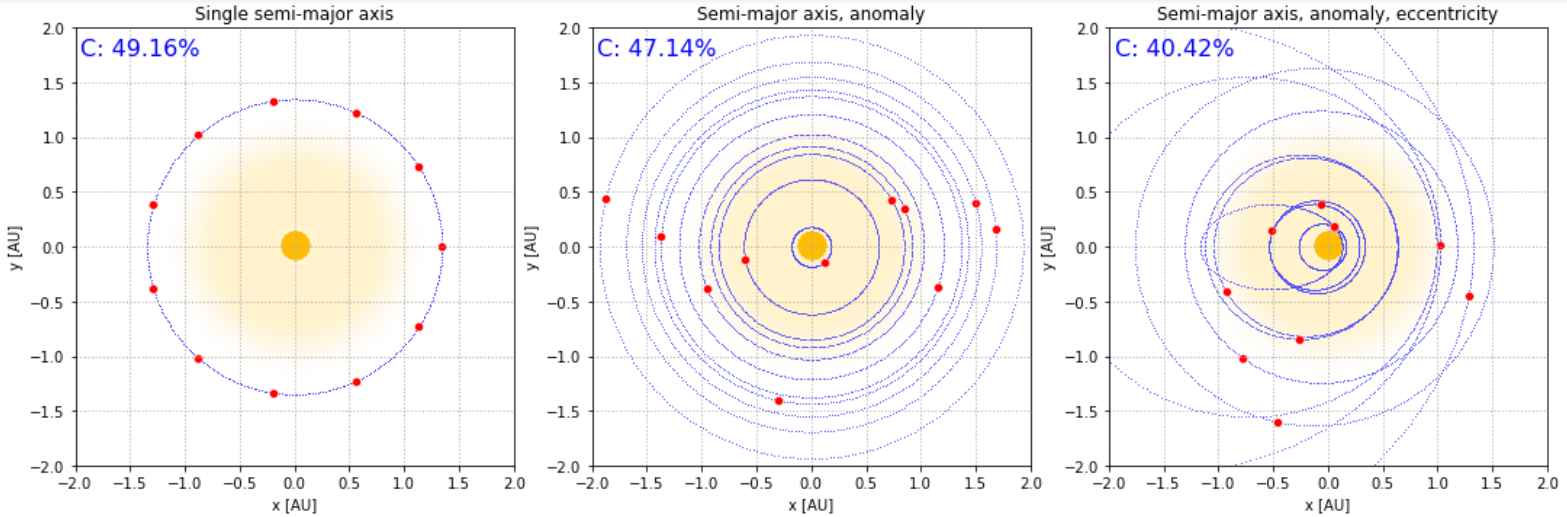
\includegraphics[width=1.0\textwidth]{img/orbits_11.png}
 \caption{Optimization results for systems with eleven spacecraft.}
 \label{fig:orbits_11}
\end{figure}
\begin{figure}[htbp]
 \centering
 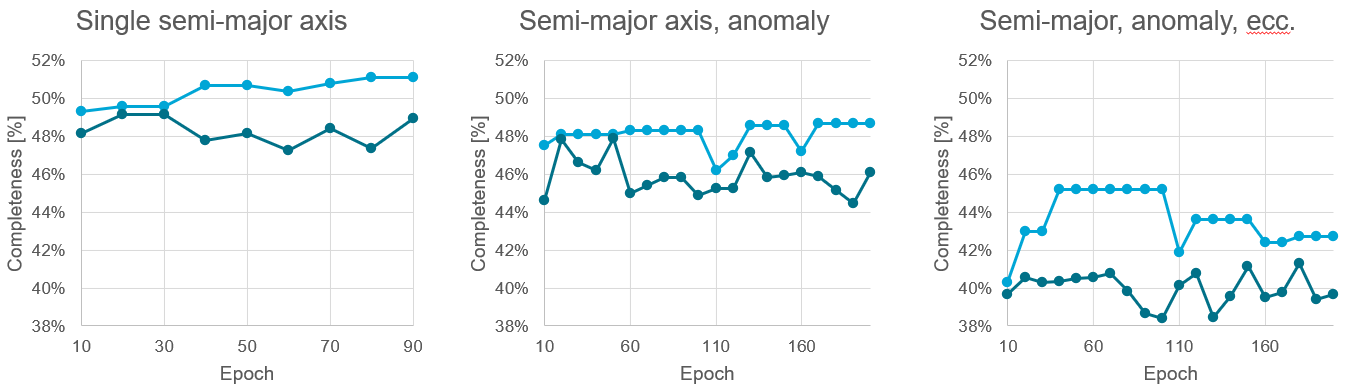
\includegraphics[width=1.0\textwidth]{img/val_orbits_11.png}
 \caption{Learning/validation results for systems with eleven spacecraft.}
 \label{fig:val_orbits_11}
\end{figure}


\section{Explanation of Observed Phenomena}
\label{sec:results_explanation}

\begin{figure}[htbp]
 \centering
 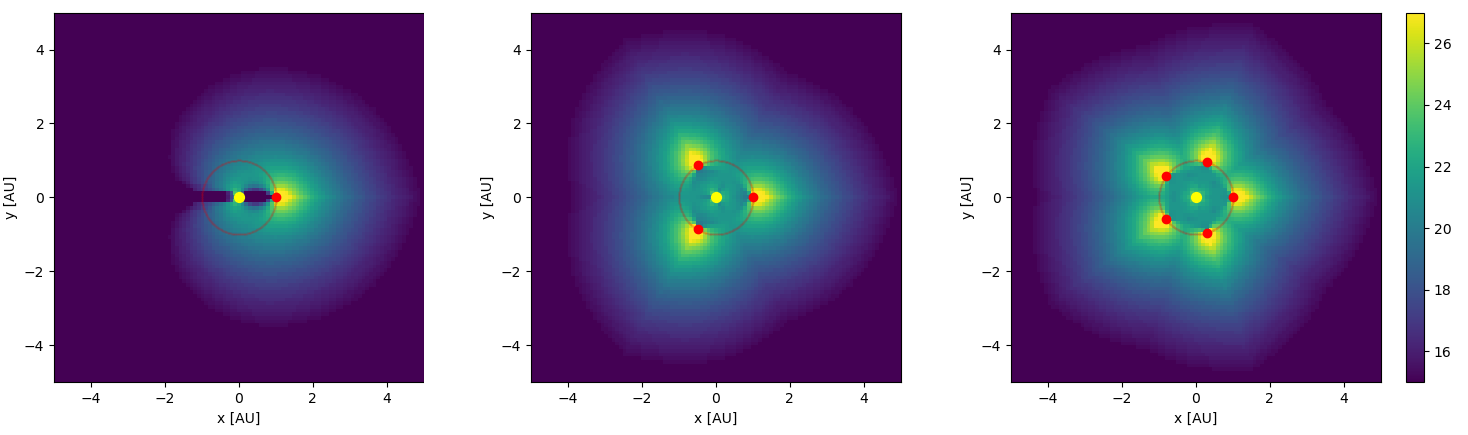
\includegraphics[width=1.0\textwidth]{img/coverage_spread.png}
 \caption{Illustration of the observable area for a system of 1, 3 and 5 spacecraft, spread out over the orbit.}
 \label{fig:coverage_spread}
\end{figure}

\begin{figure}[htbp]
 \centering
 \includegraphics[width=1.0\textwidth]{img/coverage_right.png}
 \caption{Illustration of the observable area for a system of 1, 3 and 5 spacecraft, spread apart by 0.2 rad.}
 \label{fig:coverage_tight}
\end{figure}

\begin{figure}[htbp]
 \centering
 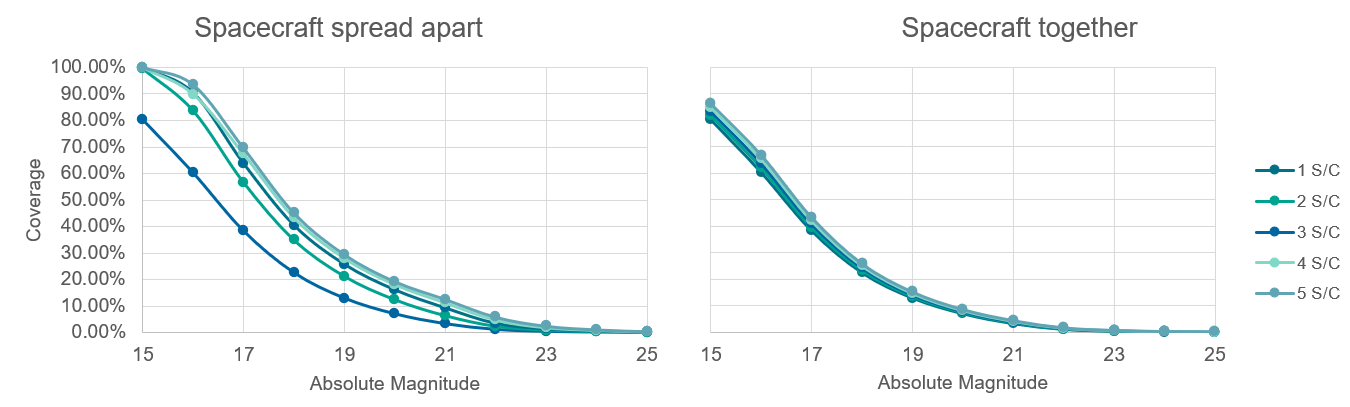
\includegraphics[width=1.0\textwidth]{img/spread_coverage.png}
 \caption{Relationship between coverage and asteroid absolute magnitude for spacecraft spread maximally apart, or spread only 0.2 rad}
 \label{fig:spread_coverage}
\end{figure}

\begin{figure}[htbp]
 \centering
 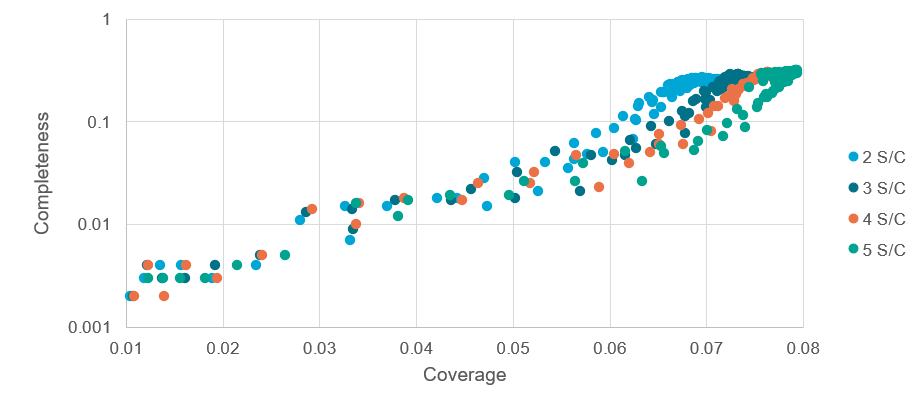
\includegraphics[width=1.0\textwidth]{img/coverage_completeness.png}
 \caption{Relationship between coverage and completeness for 2-5 spacecraft.}
 \label{fig:coverage_completeness}
\end{figure}

\begin{figure}[htbp]
 \centering
 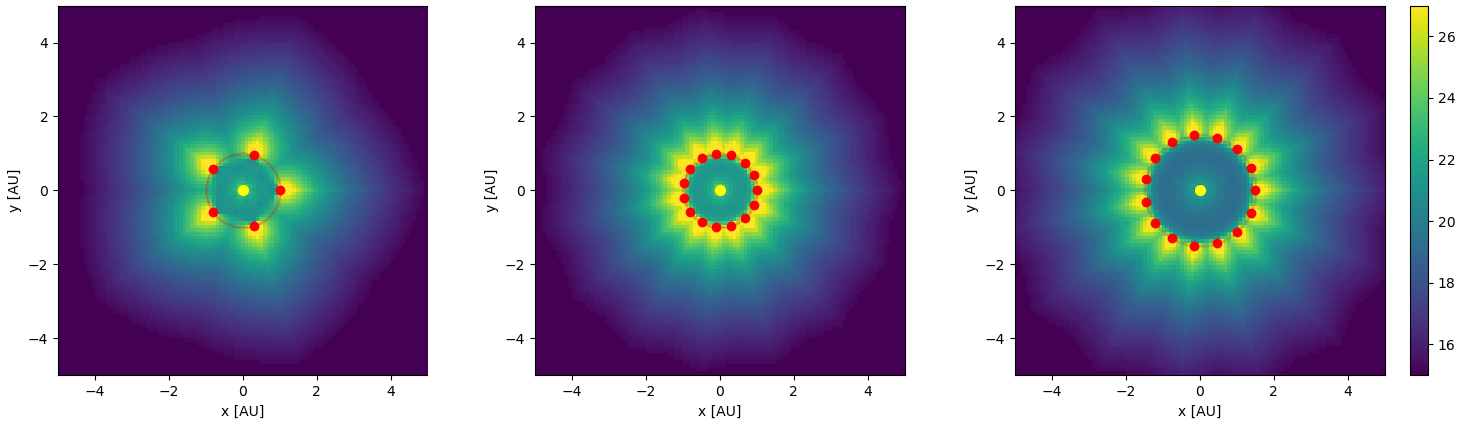
\includegraphics[width=1.0\textwidth]{img/coverage_high_n.png}
 \caption{Illustration of the observable area for a system of 15 spacecraft, at a=1.0 AU and a=1.5AU, spread out over the orbit. The 5 spacecraft case is shown for comparison.}
 \label{fig:coverage_high_n}
\end{figure}

\begin{figure}[htbp]
 \centering
 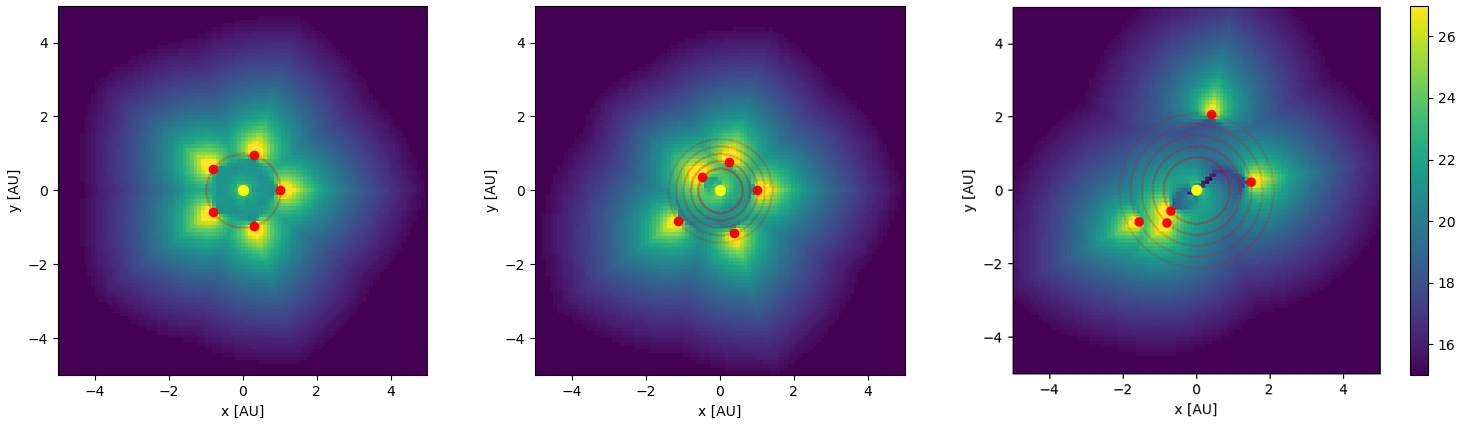
\includegraphics[width=1.0\textwidth]{img/coverage_free.png}
 \caption{Illustration of the observable area for a system of 5 spacecraft, spread out over the orbit. The left case has the spacecraft co-orbital. In the middle case, the spacecraft are in different orbits, but spread out. On the right, they have lined up in their orbital motion.}
 \label{fig:coverage_free}
\end{figure}




\section{Predicted Performance and Implications for Missions Design}
\label{sec:results_performance}



\begin{figure}[htbp]
 \centering
 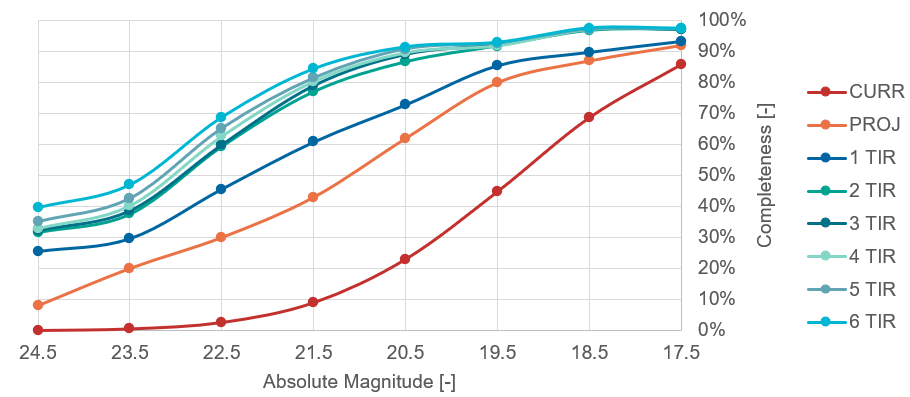
\includegraphics[width=0.9\textwidth]{img/performance_prediction.png}
 \caption{Prediction of performance}
 \label{fig:performance_prediction}
\end{figure}

\begin{figure}[htbp]
 \centering
 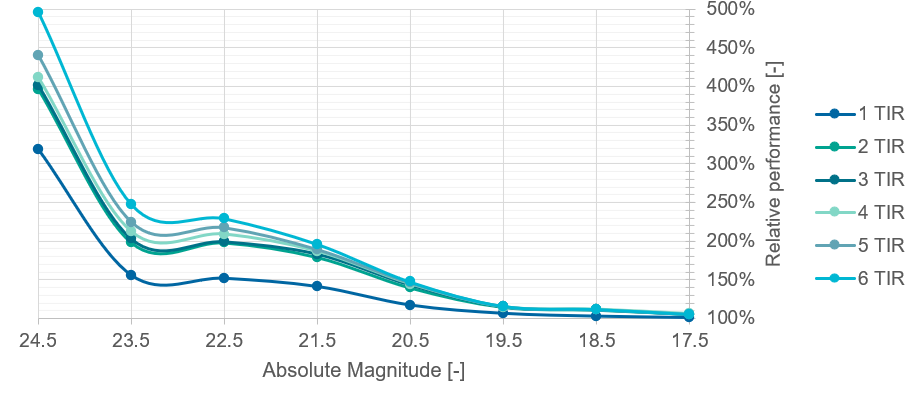
\includegraphics[width=0.9\textwidth]{img/performance_prediction_rel.png}
 \caption{Relative prediction of performance}
 \label{fig:performance_prediction_rel}
\end{figure}


20\%: 1
30\%: 2
40\%: 6
50\%: 15
60\%: 50
70\%: 200

\begin{figure}[htbp]
 \centering
 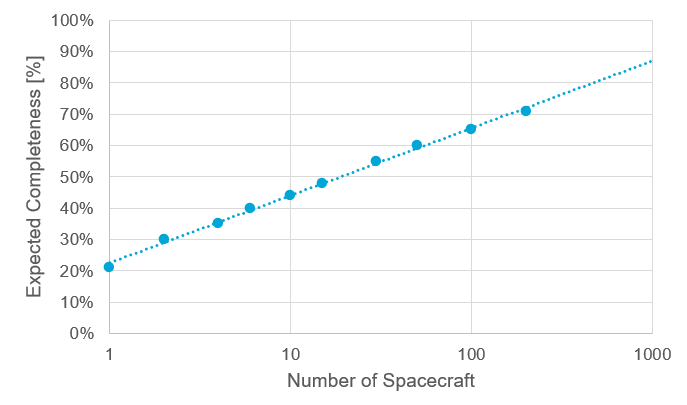
\includegraphics[width=0.7\textwidth]{img/completeness_hypothetical.png}
 \caption{Expected performance as a function of number of spacecraft.}
 \label{fig:completeness_hypothetical}
\end{figure}



\newpage
\chapter{Verification and Validation}
\label{ch:vandv}
Simulations are a useful, efficient and cost-effective way to obtain insight into complex problems, such as the one described in this report. However, care must be taken to ensure that the simulation is free of errors, and that it provides an accurate representation of reality. This process is referred to as verification and validation. \\

As described earlier, verification through unit and integration testing was performed throughout the implementation process. As can be seen in the implementation \href{https://github.com/ArjanVermeulen97/thesis-code.git}{on Github}, the code is structured into smaller unit functions, such as rotation matrices, angle calculation functions, and fundamental equations such as Planck's law. These unit functions are integrated into more complex functions, such as reference frame transformations. This approach allows for manual testing of the software from the beginning of programming to ensure correctness of the simulation. In addition, throughout the process, several sources from literature were implemented. As these sources often do not provide details as to how to implement their findings, the resulting implementation should be checked against the data in the sources. This is especially important in the case of numerical integration schemes, where accuracy can be dependent on implementation. Therefore, further verification of the thermal infrared target and background signal is presented in \autoref{sec:vvinfrared}, and the algorithm for solving the orbital positions in \autoref{sec:vvsurvey}.\\

Verification of the software units and their implementation, however, is not enough to provide acceptable results. It also has to be shown that the simulation accurately portrays the problem being studied. In particular, the effect of major assumptions, as well as the results of the system for various test cases, should be examined. To this end, the possibly impactful assumption regarding survey cadence (as discussed in \autoref{sec:methodologyimplementation}) is checked. Finally, the results of the simulation tool are compared to the results of a previously validated simulation tool - the tool developed by \cite{2017NEOSDT} - to determine whether the results presented are an accurate representation of reality. This analysis is presented in \autoref{sec:vvperformance}.

\section{Infrared Signal}
\label{sec:vvinfrared}

\begin{figure}[htbp]
 \centering
 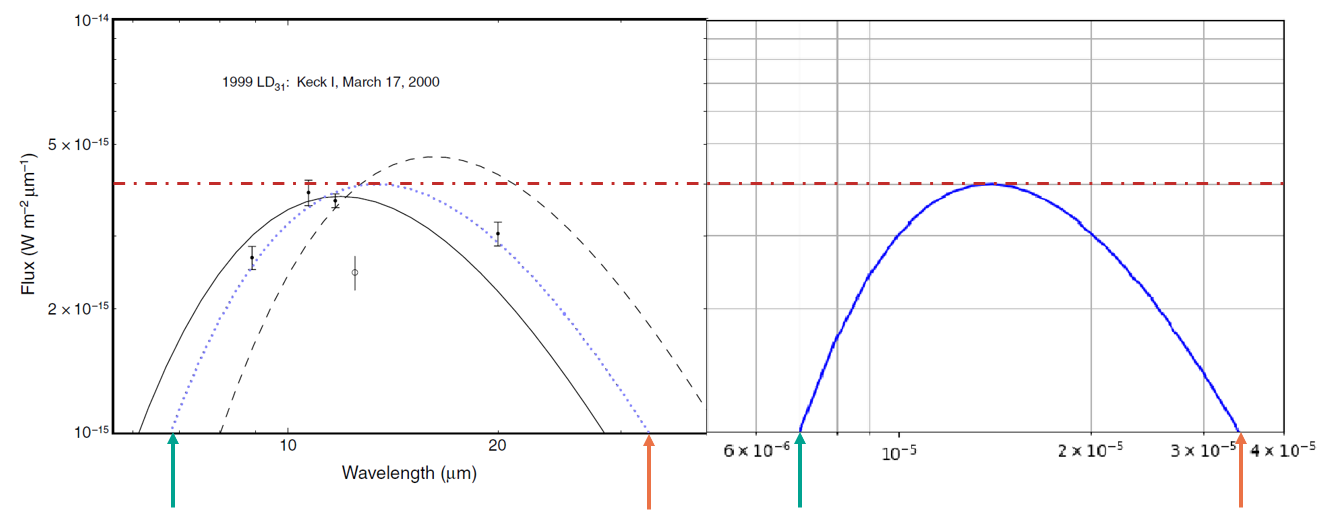
\includegraphics[width=0.9\textwidth]{img/validation_tir_target_signal.png}
 \caption{Comparison of infrared signal calculation. Reference data is shown on the left, obtained from \cite{AsteroidNEATM}. The other two curves in the plot were results of other, older, asteroid thermal models.}
 \label{fig:validation_tir_target_signal}
\end{figure}

For verification of the thermal infrared target signal, \cite{AsteroidNEATM} provide flux calculations for the asteroid 1999 LD$_{31}$, on a given date. Implementation of the thermal model was verified by repeating this simulation, and comparing the results. This comparison can be seen in \autoref{fig:validation_tir_target_signal}. Ephemeris was obtained \href{https://ssd.jpl.nasa.gov/tools/sbdb\_lookup.html#/?sstr=1999\%20LD31}{from NASA/JPL Small-Body Database}. The implementation provides the correct general shape of the curve, as well as correct maximum value and axis intercepts. Therefore it was concluded that the implementation is correct.\\

\begin{figure}[ph]
 \centering
 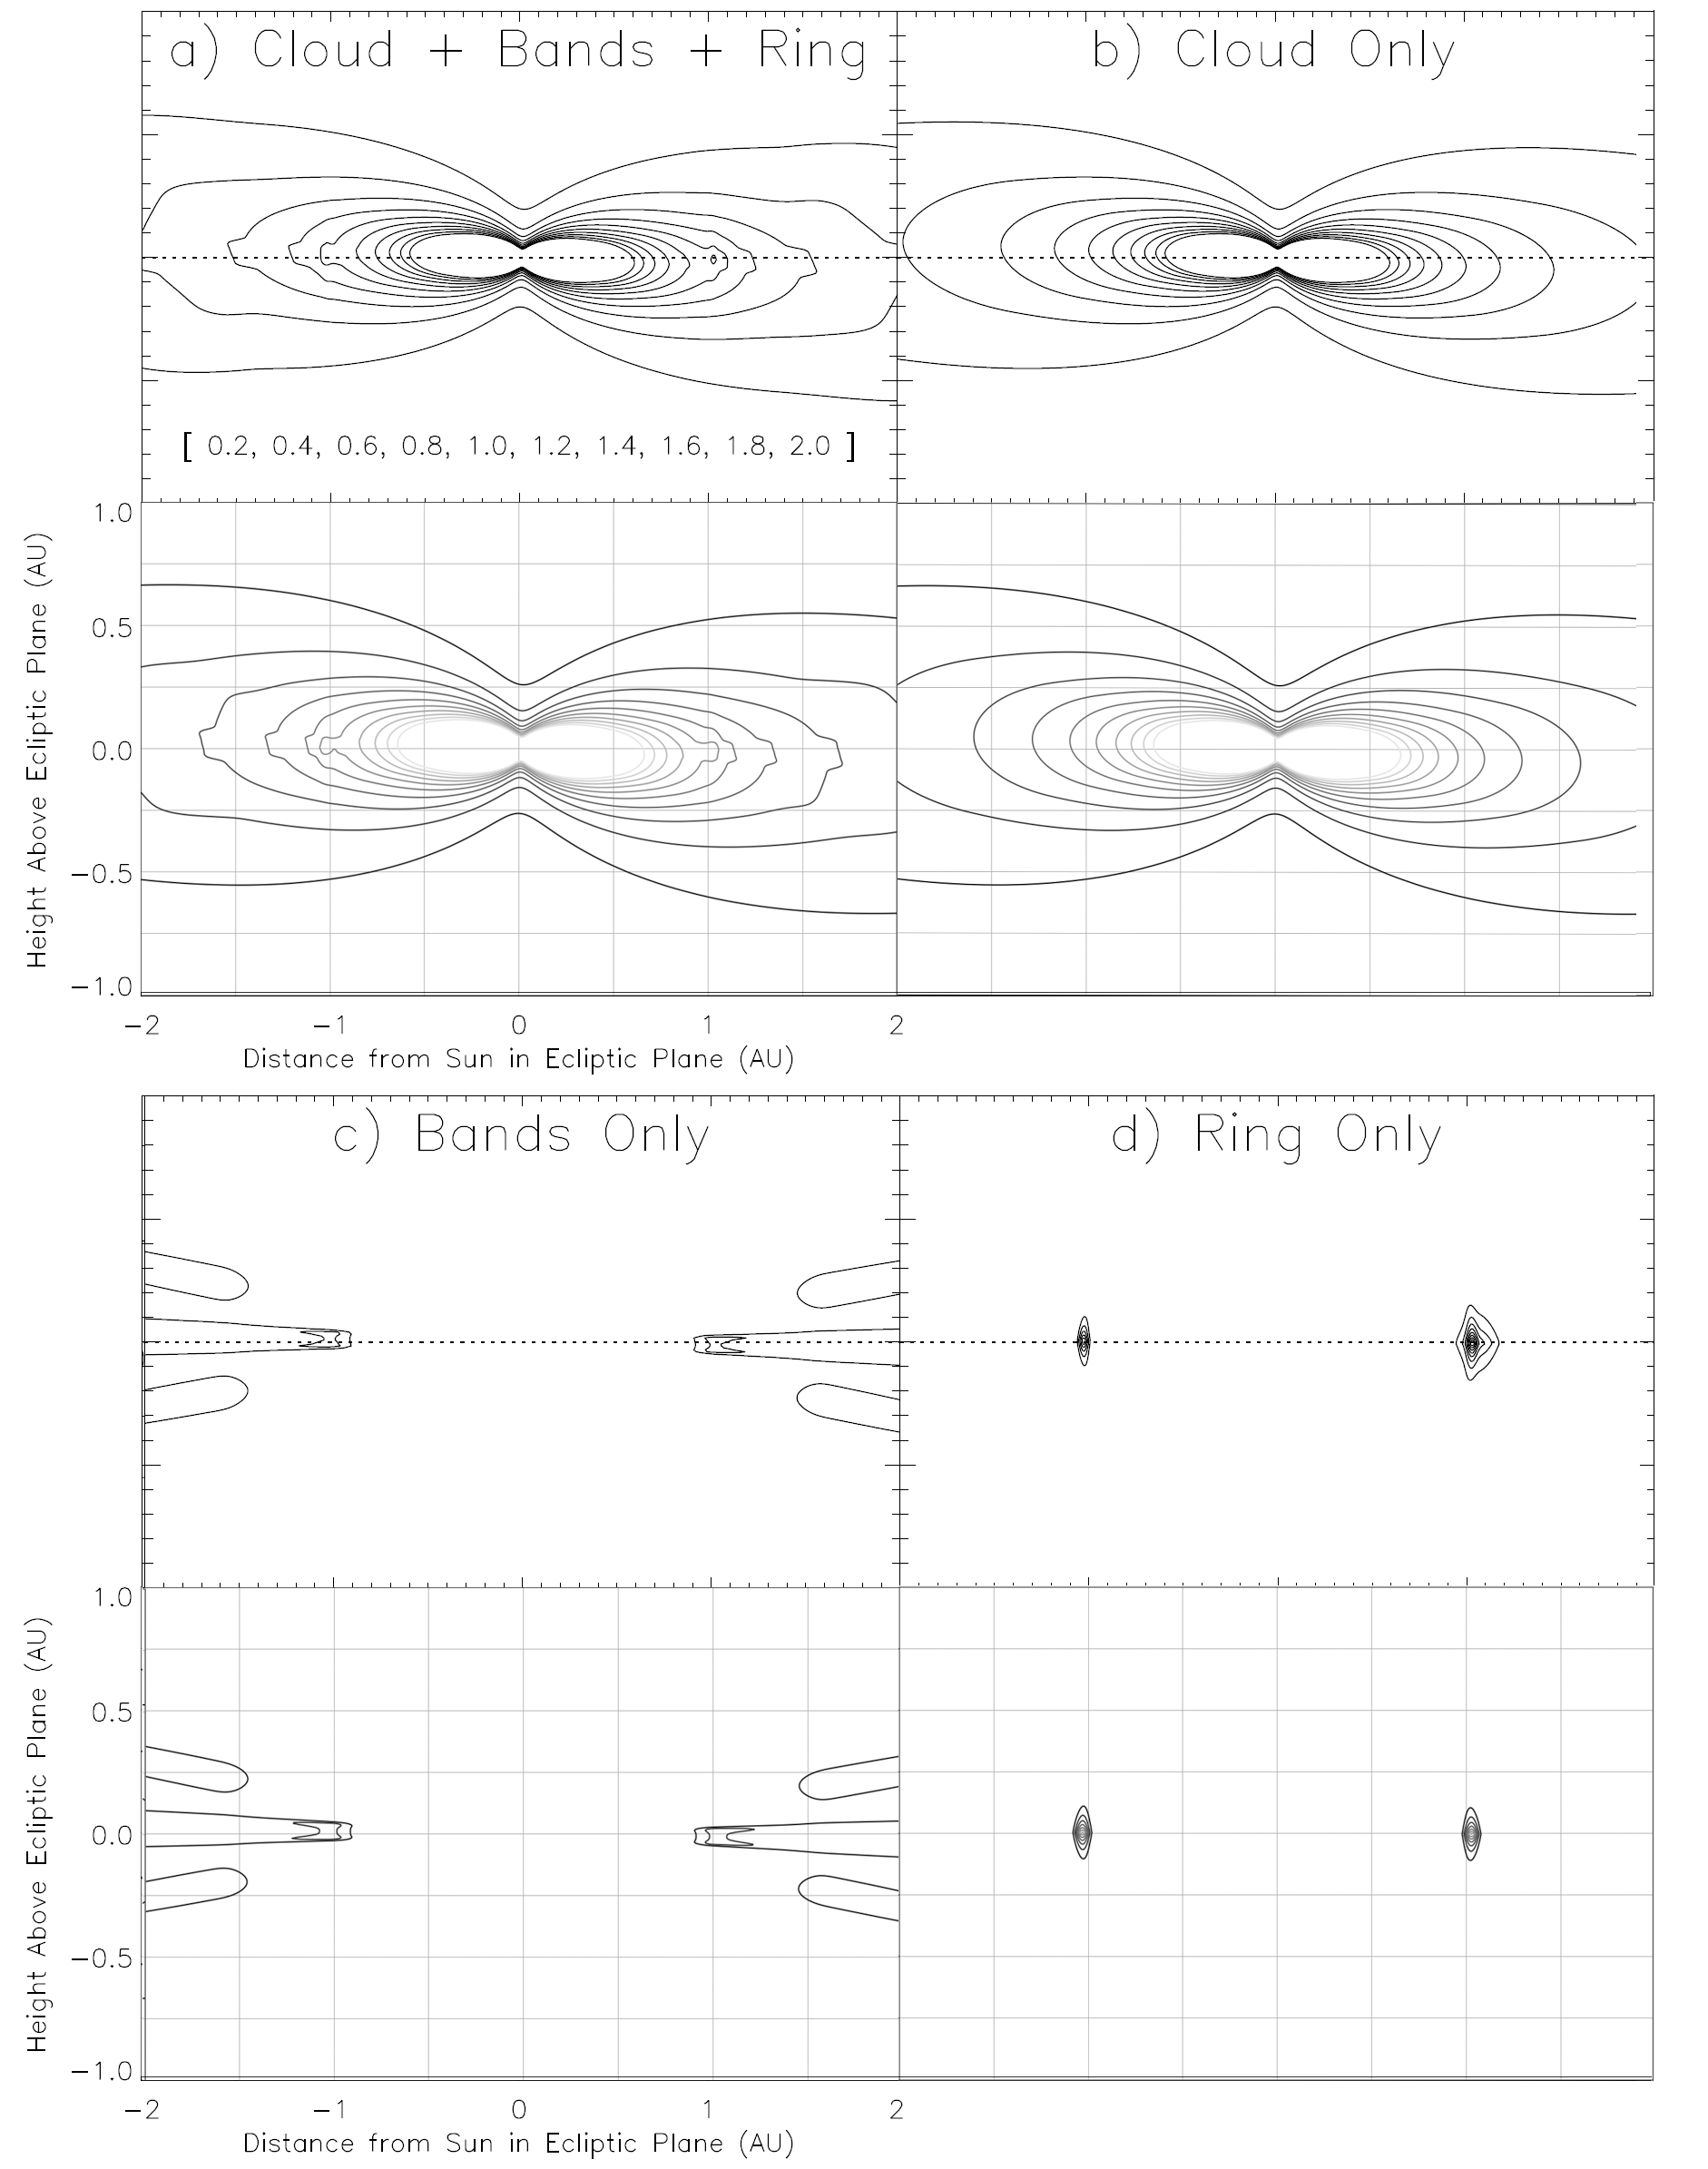
\includegraphics[width=1.0\textwidth]{img/validation_tir_background_signal.png}
 \caption{Comparison of the calculated densities of the various interplanetary dust components. Top: reference images from \cite{IRDust}, bottom: calculated densities.}
 \label{fig:validation_tir_background_signal}
\end{figure}

The second component of the infrared signal to be verified is the implementation of the interplanetary dust model provided by \cite{IRDust}. This process was conducted in two steps. Firstly, the calculated density models involve several complicated formulae, and are therefore subject to error. These were compared to implementation by \cite{IRDust} in \autoref{fig:validation_tir_background_signal}. It can be seen that the implementation matches the results of the authors. \\

\begin{table}[htbp]
\centering
\caption{Comparison of computed and reference values for the infrared zodiac light signal at $4.9\mu$m. Reference values according to \cite{IRDust}}
\label{tab:49irbackground}
\begin{tabular}{lll|l|lll}
($\lambda$, $\beta$)    & Date     & $\lambda_{\odot}$  & Component & Reference & Computed & Difference \\ \hline
122, 0  & 19-04-90 & 208.81 & Cloud     & 0.679     & 0.655    & -3.53\%    \\
        &          &        & Bands     & 0.0141    & 0.0121   & -14.2\%    \\
        &          &        & Ring      & 0.0164    & 0.0493   & 201\%      \\ \hline
        &          &        & Total     & 0.808     & 0.716    & -11.4\%    \\ \hline
137, 46 & 09-05-90 & 228.25 & Cloud     & 0.449     & 0.492    & 9.58\%     \\
        &          &        & Bands     & 0.0014    & 0.00102  & -27.1\%    \\
        &          &        & Ring      & 0.0251    & 0.00871  & -65.3\%    \\ \hline
        &          &        & Total     & 0.476     & 0.501    & 5.25\%    
\end{tabular}
\end{table}

\begin{table}[htbp]
\centering
\caption{Comparison of computed and reference values for the infrared zodiac light signal at $12\mu$m. Reference values according to \cite{IRDust}}
\label{tab:12irbackground}
\begin{tabular}{lll|l|lll}
($\lambda$, $\beta$)    & Date     & $\lambda_{\odot}$  & Component & Reference & Computed & Difference \\ \hline
122, 0  & 19-04-90 & 208.81 & Cloud     & 28.476    & 29.63    & 4.05\%     \\
        &          &        & Bands     & 1.938     & 1.78     & -8.15\%    \\
        &          &        & Ring      & 3.324     & 1.6      & -51.9\%    \\ \hline
        &          &        & Total     & 33.875    & 33.011   & -2.55\%    \\ \hline
137, 46 & 09-05-90 & 228.25 & Cloud     & 14.669    & 17.208   & 17.3\%     \\
        &          &        & Bands     & 0.0924    & 0.0868   & -6.06\%    \\
        &          &        & Ring      & 0.735     & 0.266    & -63.8\%    \\ \hline
        &          &        & Total     & 15.483    & 17.561   & 13.4\%    
\end{tabular}
\end{table}

The second step is required for judging the accuracy of the various numerical integrations involved in the model. This was done using reference values provided by the authors. The calculated and reference contributions for the various components in the two test cases can be seen in \autoref{tab:49irbackground} for the $4.9 \mu\mathrm{m}$ wavelength and \autoref{tab:12irbackground} for the $12 \mu\mathrm{m}$ background. Ephemerides were obtained \href{https://ssd.jpl.nasa.gov/horizons/}{from NASA/JPL Horizons System}. It can be seen in the tables that the error of the implementation is in the order of 10\%, which was deemed acceptable, given the nature of numerical integration of complicated functions. A point of note, however, is the large discrepancy in calculated values for the contribution of the circumsolar ring. This discrepancy is due to the fact that \cite{IRDust} include a contribution for an Earth-trailing blob of dust in their analysis. In the implementation presented here, this blob was omitted, as implementation of an addition Earth empheris would complicate the analysis, and impact was judged as small as the topic of interest is not - unlike the work of \cite{IRDust} - observation from Earth.

\section{Survey Implementation}
\label{sec:vvsurvey}
The second subject of additional inspection is the implementation of the survey components. Firstly, the implementation of the orbital mechanics and reference frame transformations has to be verified. In \autoref{fig:validation_theta_solve}, the modelled relationship between true anomaly and mean anomaly as a function of eccentricity is shown. The results of this are as expected (see e.g. \cite{Curtis}), meaning the algorithm for numerical approximation was implemented correctly, and works as predicted. Some cases, specifically for $e$ close to 1 and mean anomaly very close to $2\pi$ resulted in an initial guess of $\theta > 2\pi$ before differential corrections. This introduced an error in the code. For these cases it was found that setting $\theta = 2\pi$ provided a good solution. \\

\begin{figure}[htbp]
 \centering
 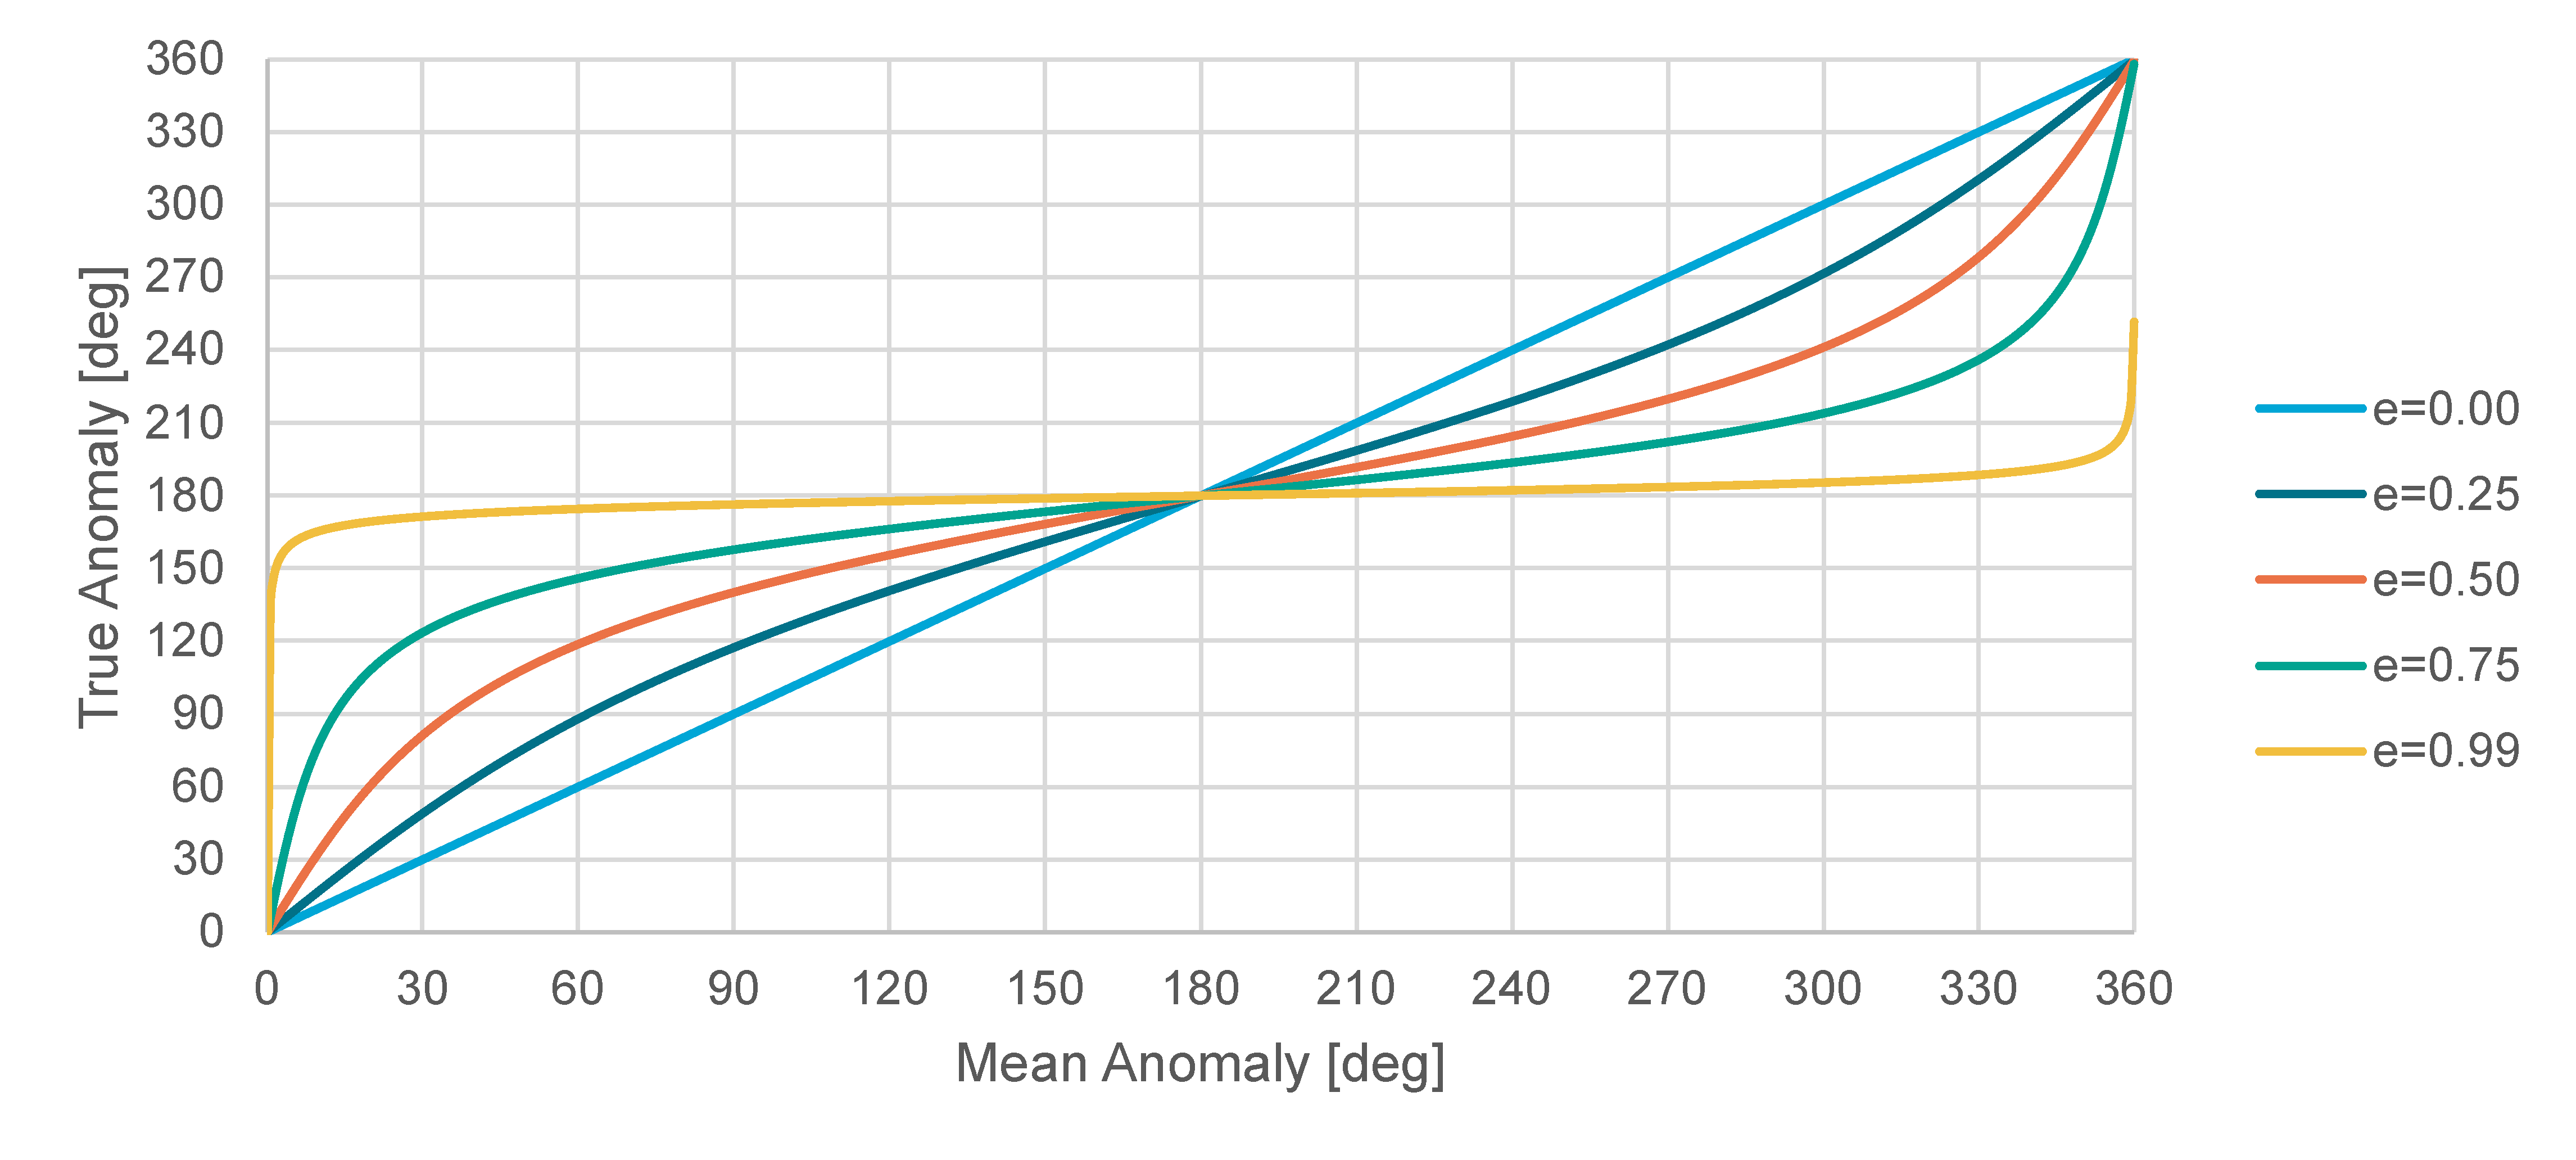
\includegraphics[width=0.8\textwidth]{img/validation_theta_solve.pdf}
 \caption{Relationship between mean anomaly and true anomaly for various eccentricities.}
 \label{fig:validation_theta_solve}
\end{figure}

The second part of the orbital propagation to be verified is the transformation from Keplerian orbital elements to cartesian coordinates. Reference frame transformations are infamously susceptible to error, and therefore a large set of reference calculations were performed for various combinations of orbital elements. A small, arbitrary, sample of these results is shown in \autoref{tab:keplertocartesian}. Distances are given in AU, angles in degrees. The transformations can be seen to be correct.\\

\begin{table}[htbp]
\centering
\caption{Comparison of computed and reference transformations from Keplerian orbital elements to cartesian coordinates.}
\label{tab:keplertocartesian}
\begin{tabular}{llllll|lll|lll}
$a$   & $e$   & $i$  & $\Omega$ & $\omega$ & $\theta$ & $x_c$      & $y_c$      & $z_c$     & $x_r$  & $y_r$  & $z_r$ \\ \hline
0.5 & 0   & 0  & 0    & 0       & 0     & 0.500  & 0.000  & 0.000 & 0.500  & 0.000  & 0.000 \\
0.5 & 0   & 90 & 180  & 90      & 90    & 0.500  & 0.000  & 0.000 & 0.500  & 0.000  & 0.000 \\
0.5 & 0.5 & 90 & 90   & 180     & 0     & 0.000  & -0.250 & 0.000 & 0.000  & -0.250 & 0.000 \\
0.5 & 0.9 & 45 & 90   & 0       & 180   & 0.000  & -0.950 & 0.000 & 0.000  & -0.950 & 0.000 \\
1   & 0   & 45 & 0    & 90      & 90    & -1.000 & 0.000  & 0.000 & -1.000 & 0.000  & 0.000 \\
1   & 0.5 & 0  & 180  & 180     & 180   & -1.500 & 0.000  & 0.000 & -1.500 & 0.000  & 0.000 \\
1   & 0.9 & 0  & 180  & 0       & 90    & 0.000  & -0.190 & 0.000 & 0.000  & -0.190 & 0.000 \\
2   & 0   & 0  & 90   & 90      & 0     & -2.000 & 0.000  & 0.000 & -2.000 & 0.000  & 0.000 \\
2   & 0   & 90 & 0    & 180     & 180   & 2.000  & 0.000  & 0.000 & 2.000  & 0.000  & 0.000 \\
2   & 0.5 & 90 & 0    & 0       & 90    & 0.000  & 0.000  & 1.500 & 0.000  & 0.000  & 1.500
\end{tabular}
\end{table}

Next, the assumption on the survey cadence will be validated. As discussed in \autoref{sec:methodologyimplementation}, this assumption was made to vastly decrease computational load, allowing numerical optimization through repeated simulations. Validation was performed through explicitly modelling the survey cadence as it would occur in reality for a range of spacecraft parameters (numerically optimizing the solutions was deemed infeasible due to the long computational time of these simulations), and comparing these to outputs of the simulation with the assumption applied. The resulting performances along with their standard deviation, is shown in \autoref{fig:validation_cadence_performance}. The error introduced by the assumption is minor, and it still accurately portrays the problem to be simulation. In fact, inspection of the difference between the simulations, shown in \autoref{fig:validation_cadence_error}, reveals the error to be in the order of 1-2\%. However, as is also shown in that figure, the variance in the results is far greater than the influence of this assumption. It is however concluded that the assumptions results in an approximate 1\% underestimation of the performance of the system, which was deemed acceptable for the benefits provided by the assumption.

\begin{figure}[htbp]
 \centering
 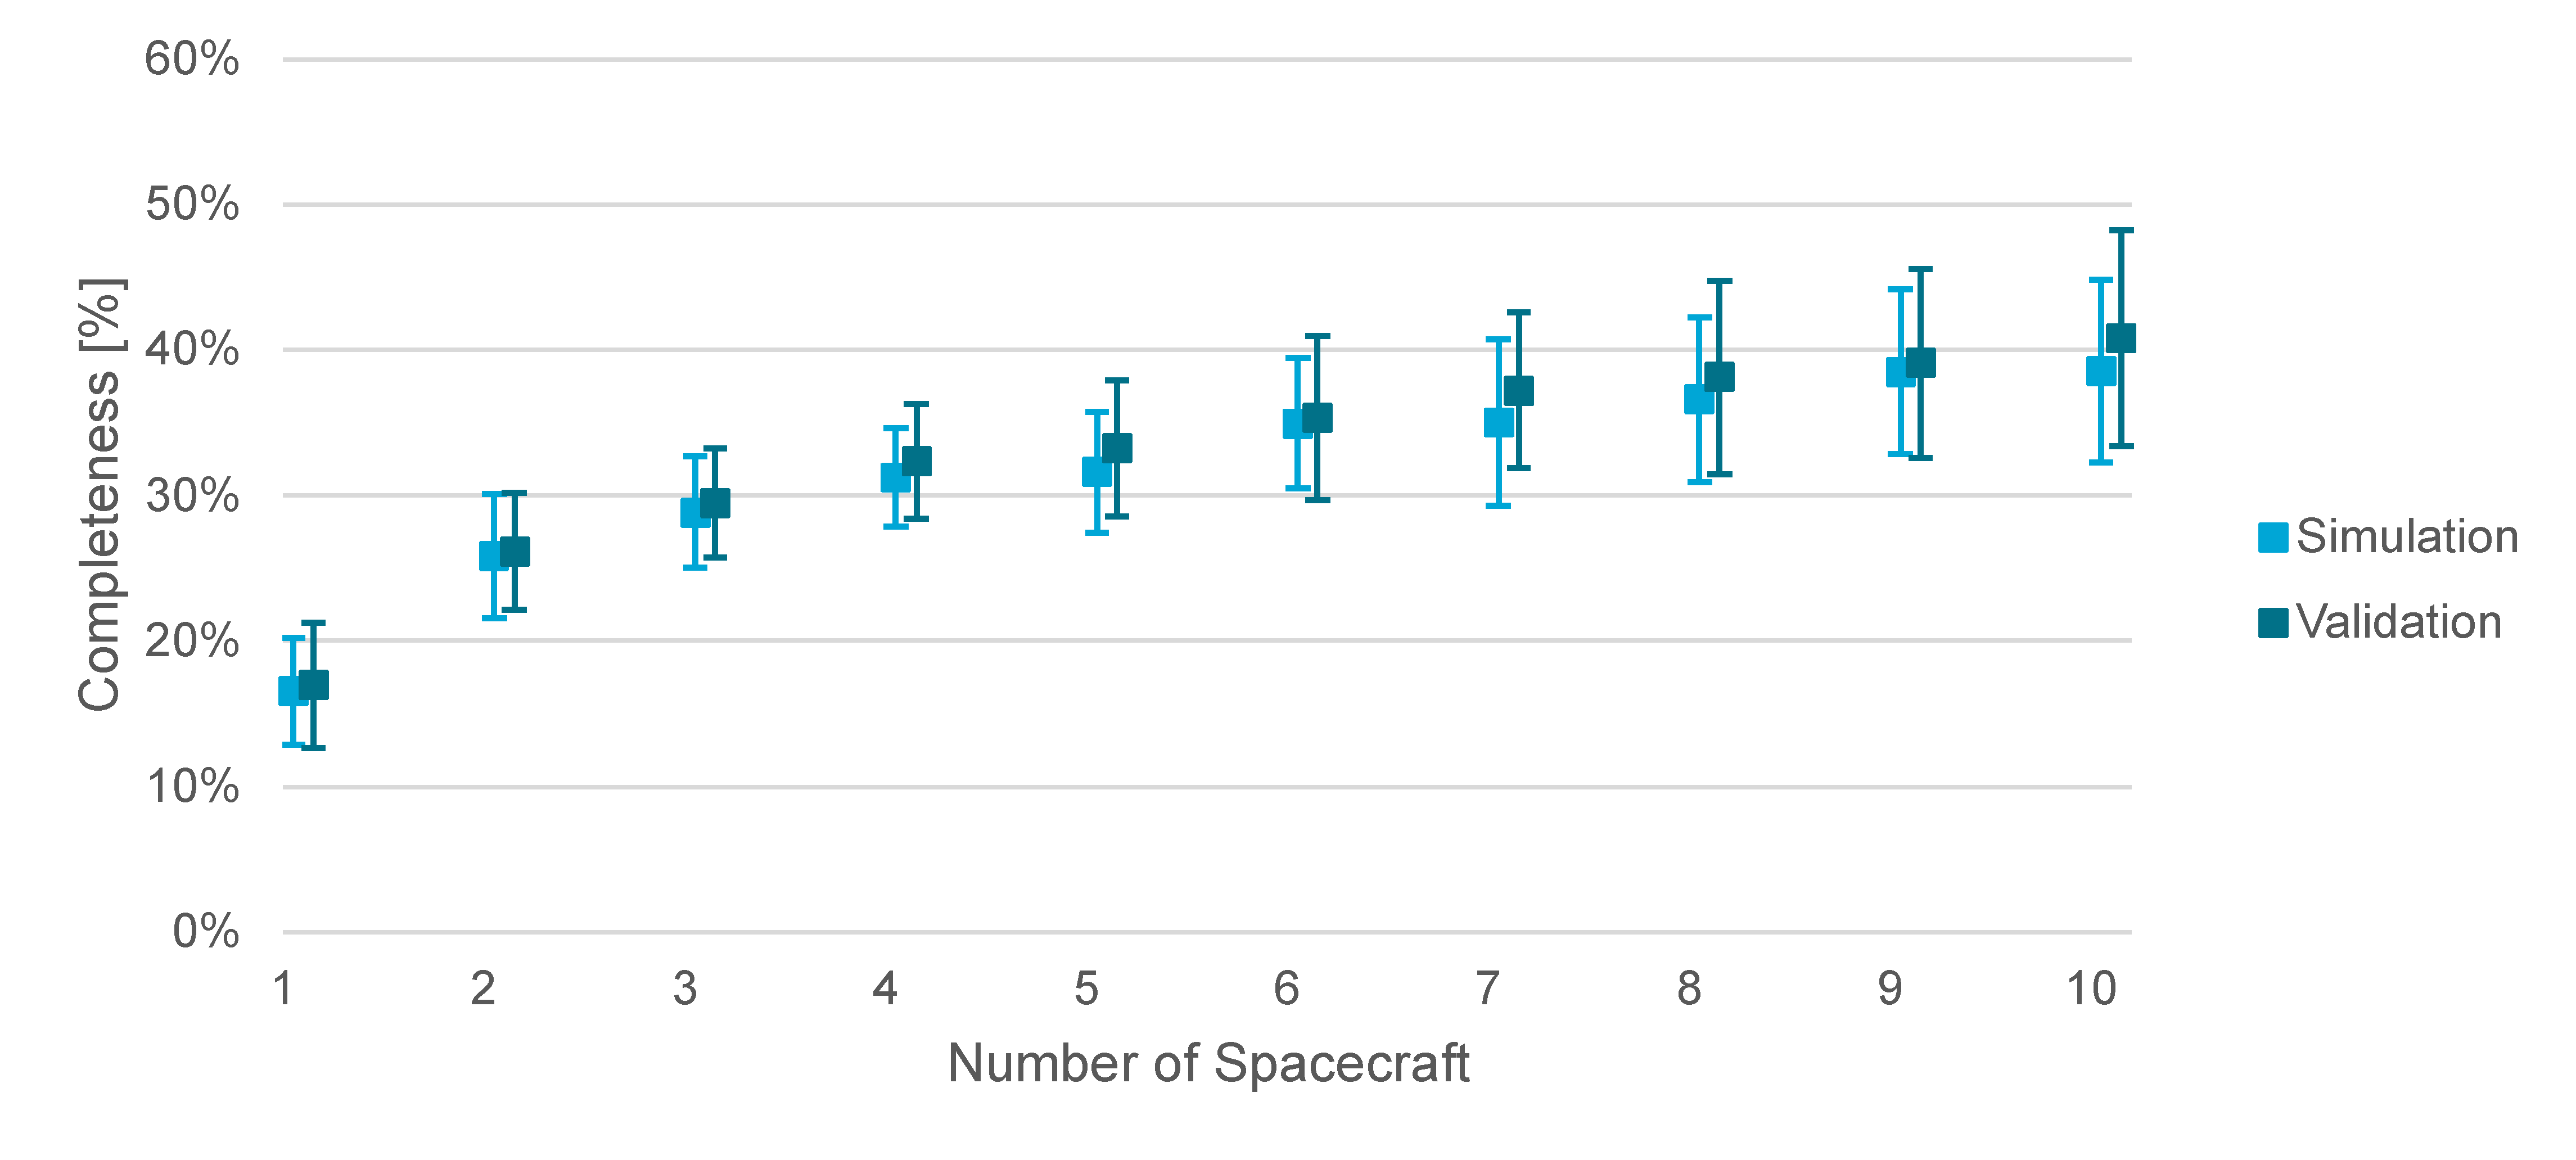
\includegraphics[width=0.8\textwidth]{img/validation_cadence_performance.pdf}
 \caption{Comparison of survey completeness with and without assumptions on survey cadence.}
 \label{fig:validation_cadence_performance}
\end{figure}

\begin{figure}[htbp]
 \centering
 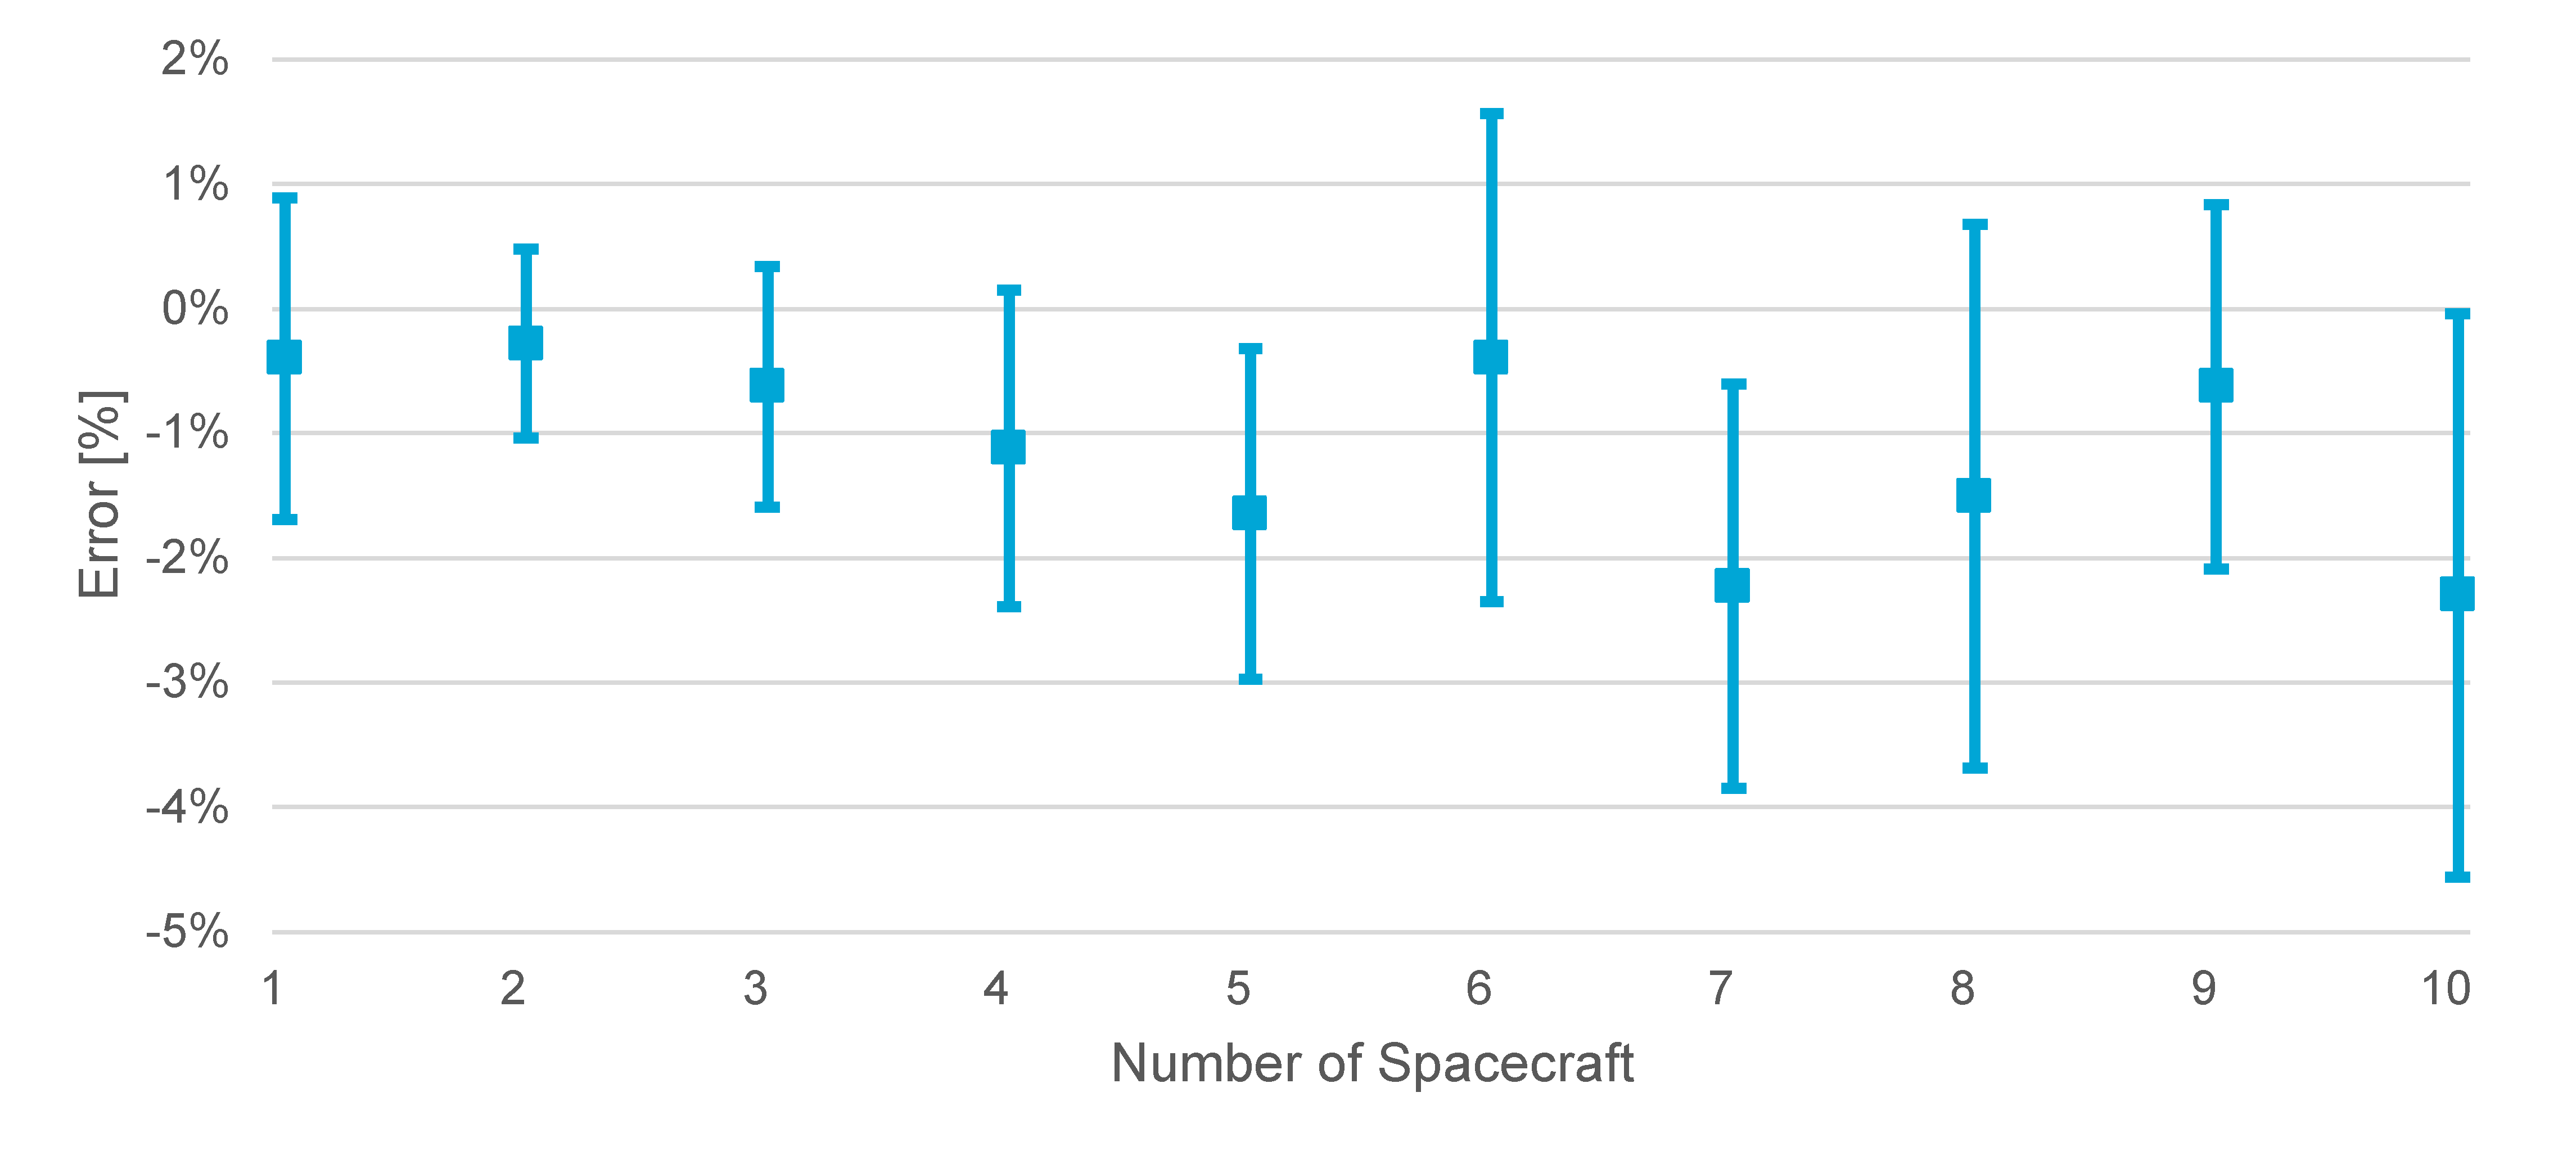
\includegraphics[width=0.8\textwidth]{img/validation_cadence_error.pdf}
 \caption{Error in survey result introduced by the assumptions on survey cadence.}
 \label{fig:validation_cadence_error}
\end{figure}

The assumption on cadence implicitly introduces another approximation, however. As the entire sky is imaged at the same time, this also means the spacecraft is imaging towards the Sun. Naturally, aiming a telescope at the Sun is generally ill-advised. Therefore in practice the spacecraft will be limited in how close it can approach the Sun in terms of angular distance. This \textit{maximum solar elongation} $\phi_{max}$ precludes the spacecraft from imaging objects near the Sun. On the other hand, as a smaller area of sky has to be imaged, the survey cadence increases proportionally. Influence of this effect was judged by excluding NEA's below a certain solar elongation from detection. Conversely, the survey cadence was increased by a factor of $\phi_{max}^2 / 4\pi$ to compensate. The results can be seen in \autoref{fig:validation_solar_angle} for $\phi_{max}$ up to $\pi/2$. Even as the number of spacecraft varies, a cut-off point around $\phi_{max} = 1\mathrm{rad}$ is presented. This occurs as most asteroids will be imaged at higher solar elongations; only very few - very large - asteroids can be detected close to the Sun, and at low $\phi_{max}$, the effect on cadence is limited. In addition, these effects have opposite effects on the survey performance, and thus the final impact is negligible.

\begin{figure}[htbp]
 \centering
 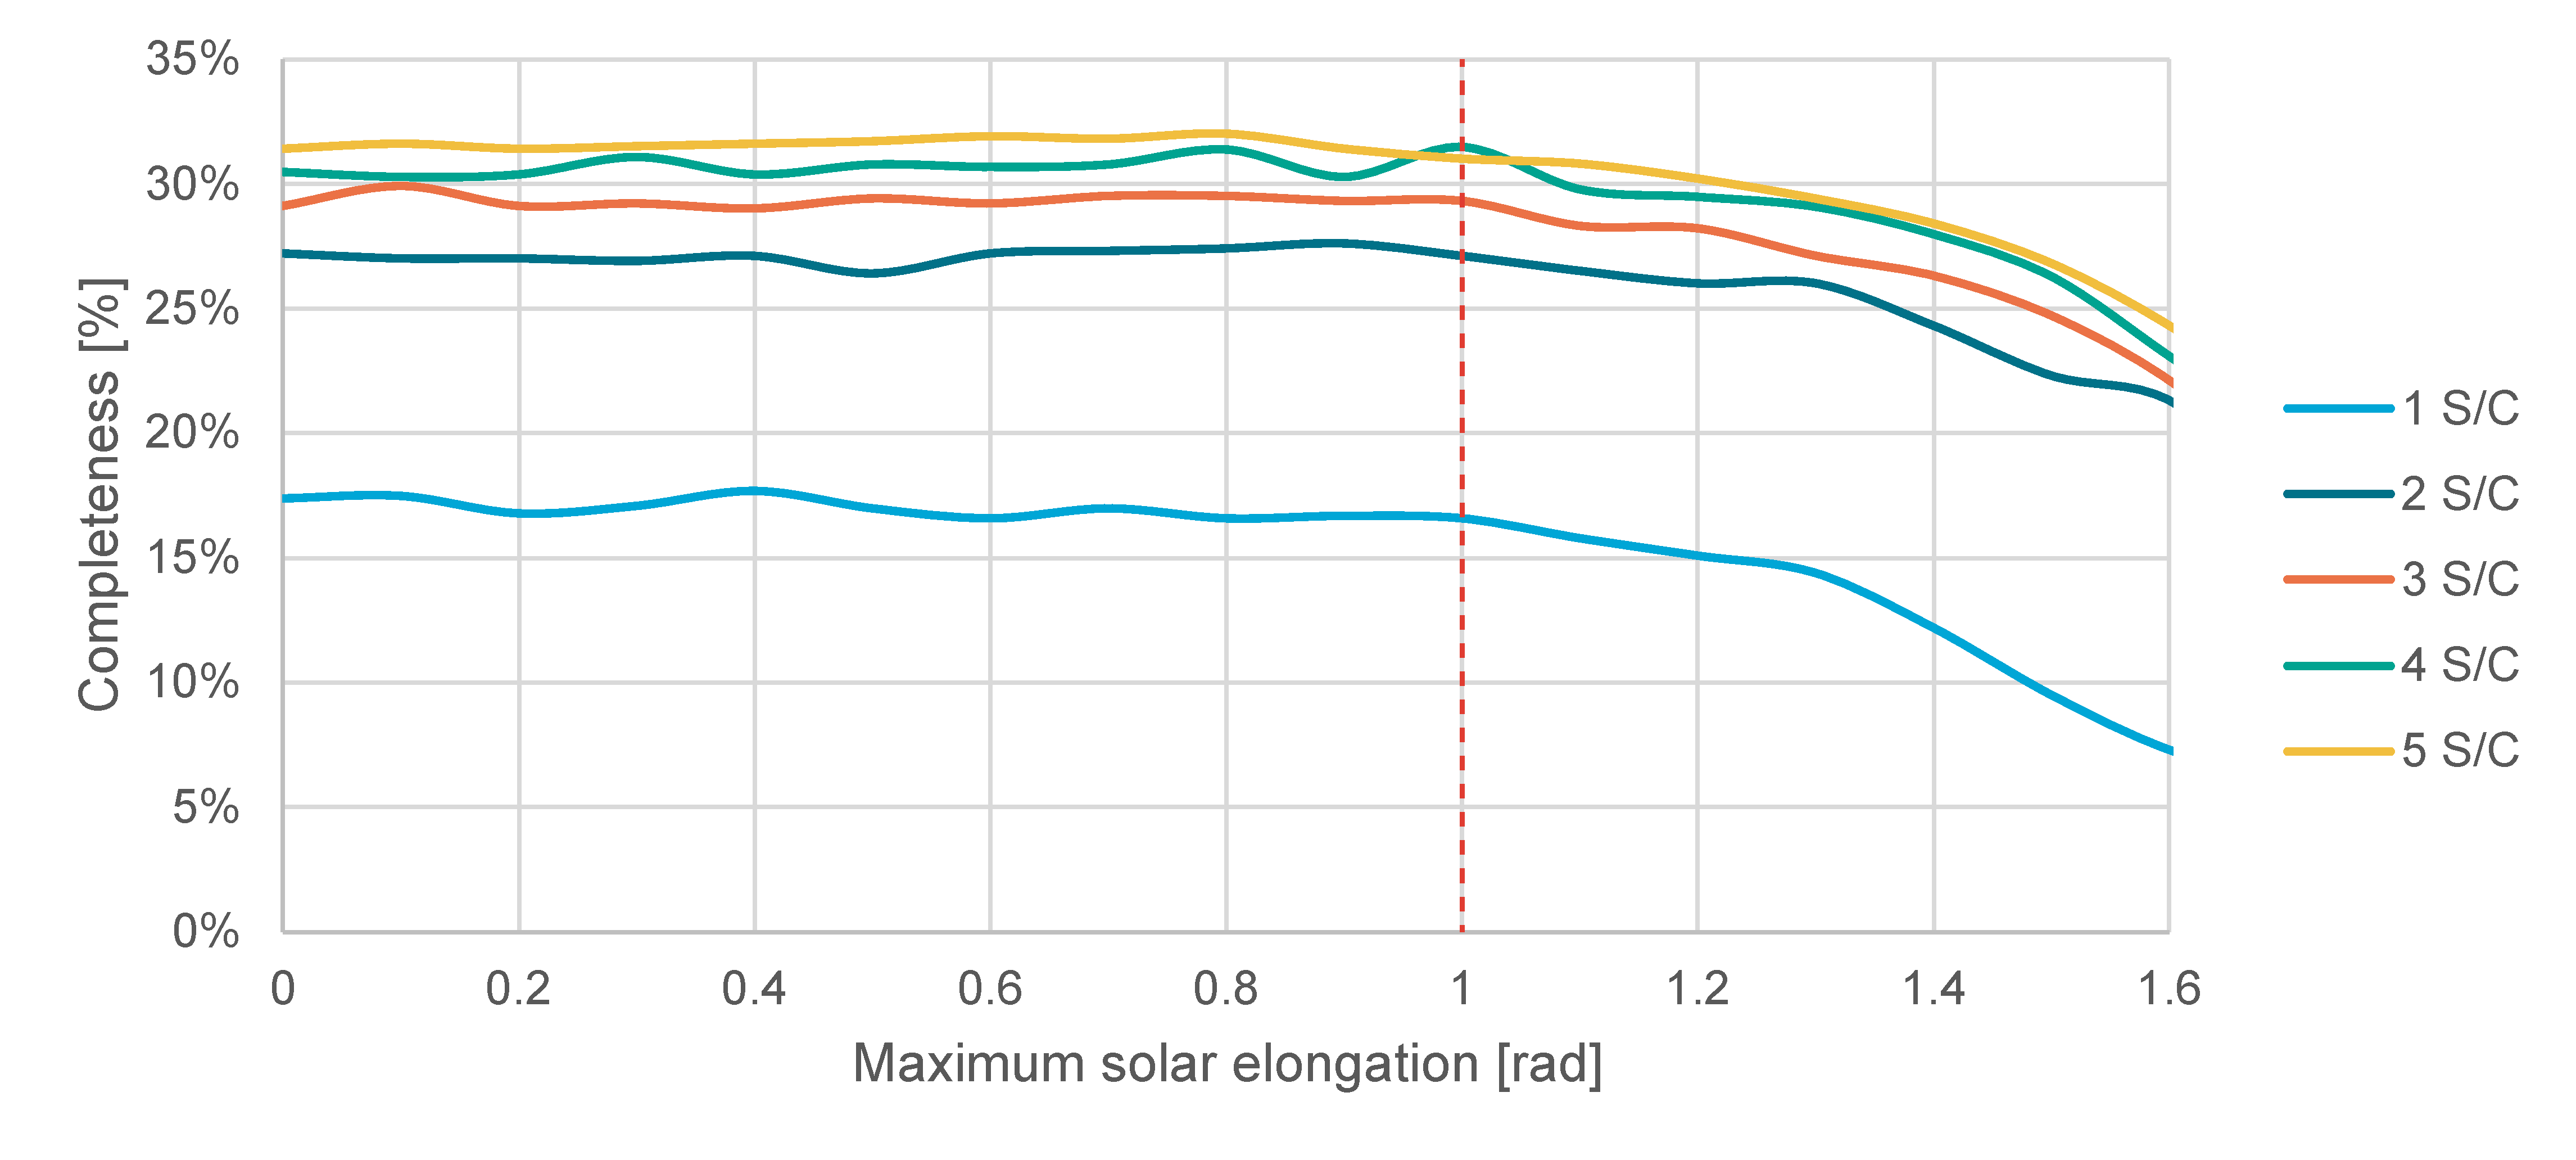
\includegraphics[width=0.8\textwidth]{img/validation_solar_angle.pdf}
 \caption{Expected survey performance as a function of maximum solar elongation.}
 \label{fig:validation_solar_angle}
\end{figure}

A final component of the simulation design has to be adressed, which is the time-dependency of the problem. As the orbits of NEA's are affected by more influences than just the Sun's gravity (see \cite{GranvikPopulation} for a full discussion of this topic), it could be the case that the distribution of asteroids is not entirely homogeneous. In these cases, situations might arise where a time-dependency is introduced into the problem. For example, surveys starting at a later date might show a higher performance than surveys starting earlier due to fluctuations in the asteroids population. Therefore, an analysis was conducted where the survey was simulated offset by a certain period. The results of this simulation can be seen in \autoref{fig:validation_starting_year} for one to four spacecraft. Naturally, some variation is present in the points due to the variance in the simulation. However, there is no significant relationship present between the starting time and the performance of the survey.

\begin{figure}[htbp]
 \centering
 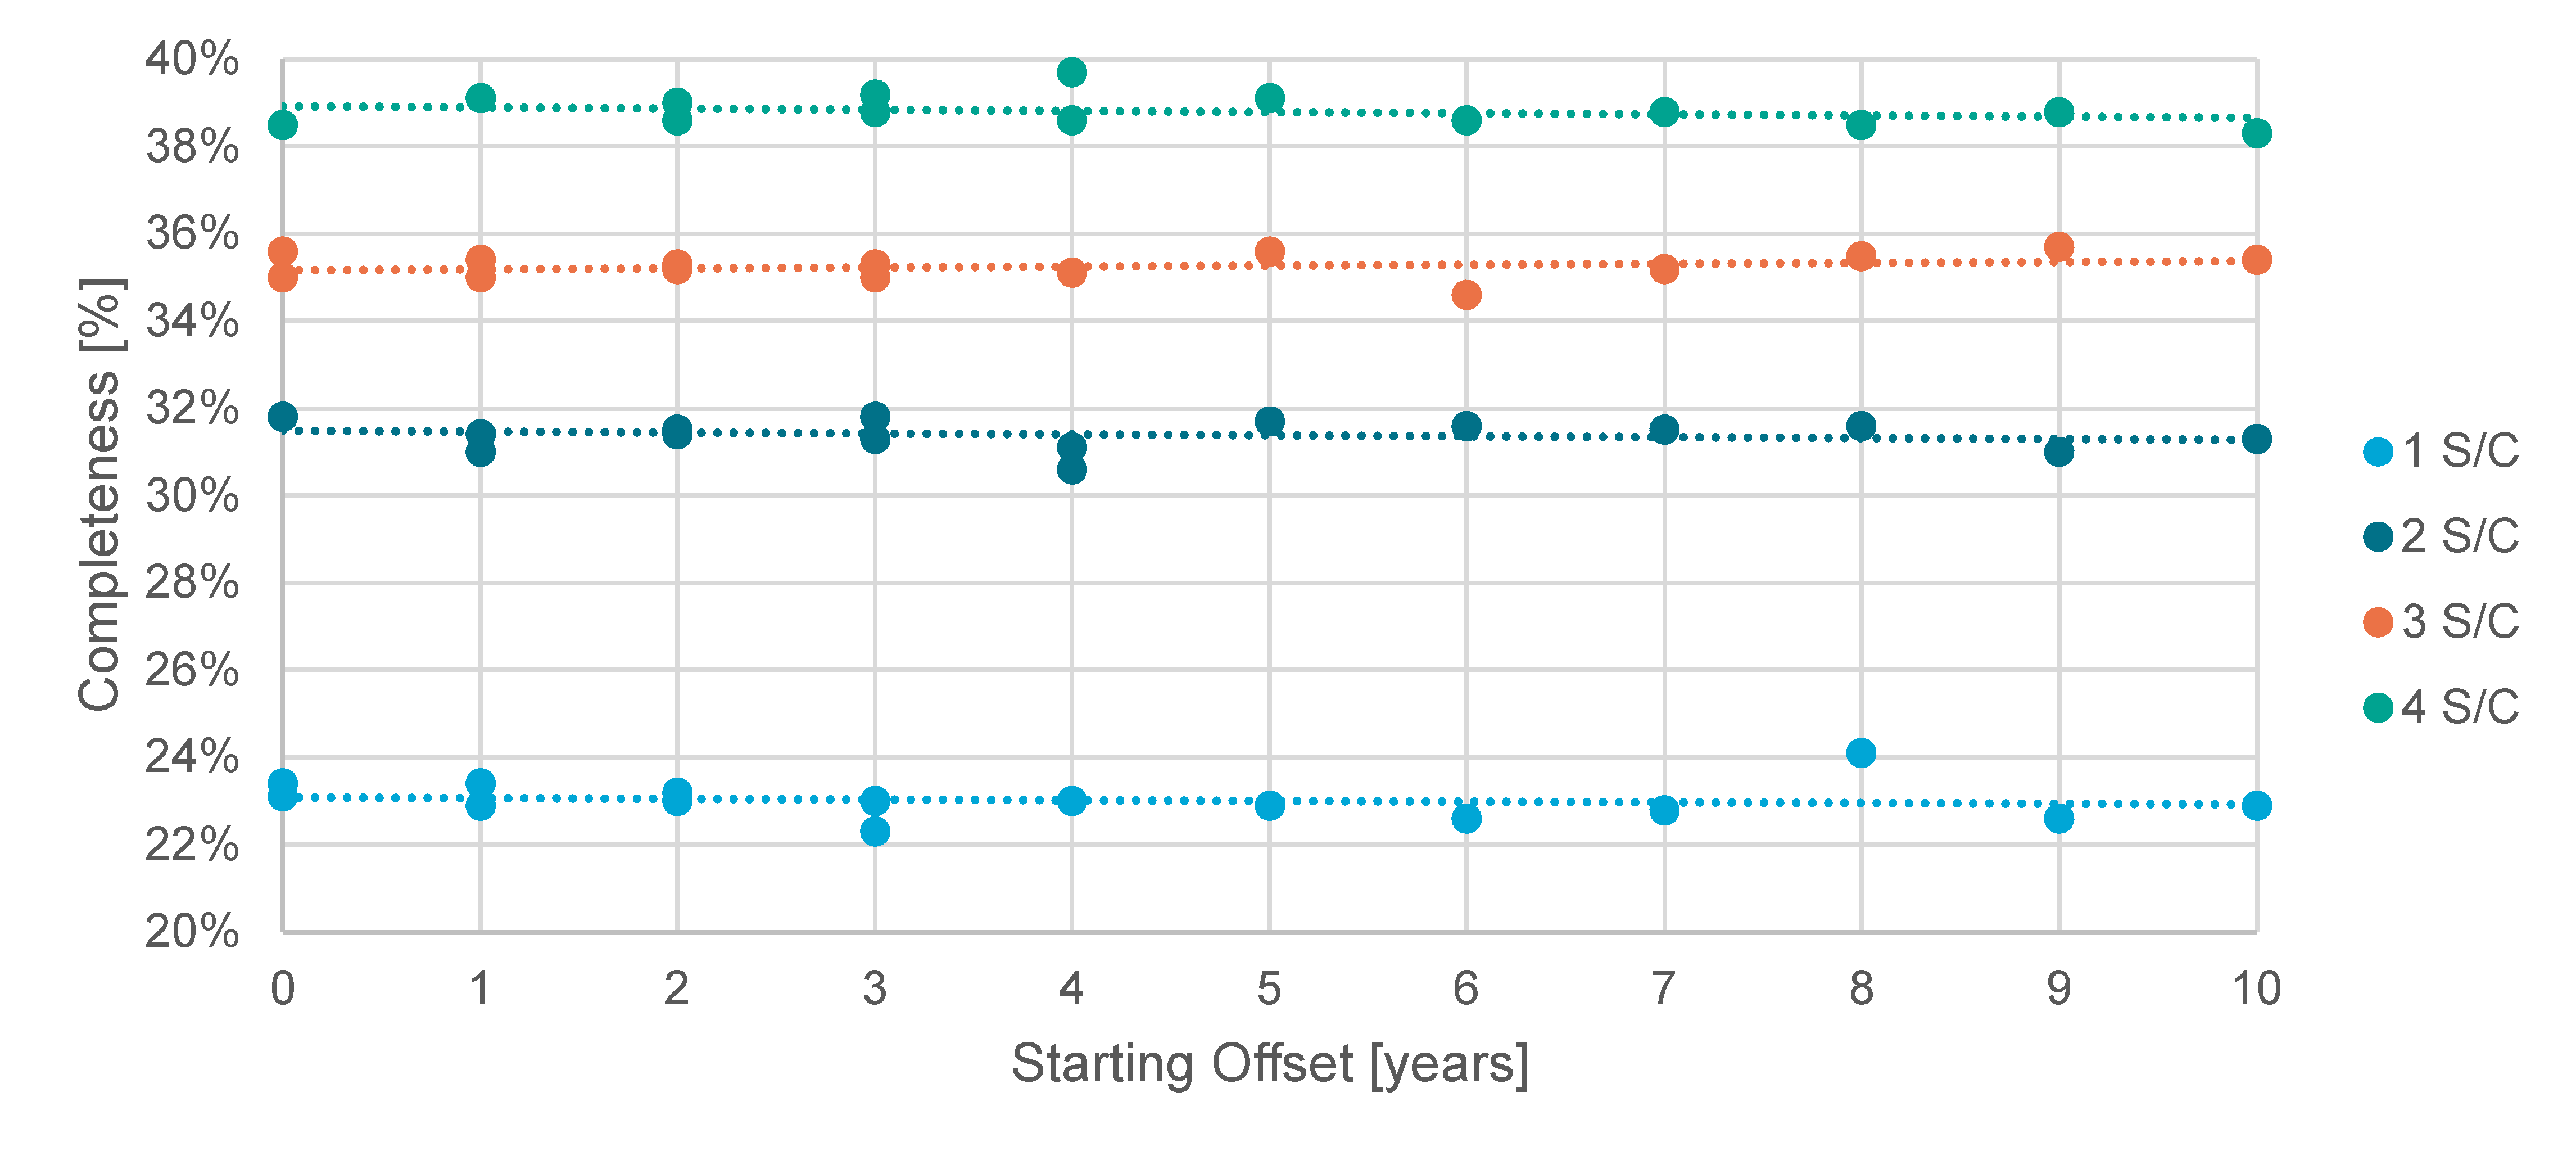
\includegraphics[width=0.8\textwidth]{img/validation_starting_year.pdf}
 \caption{Expected survey performance as a function of the offset in start date.}
 \label{fig:validation_starting_year}
\end{figure}



\section{Expected Performance}
\label{sec:vvperformance}

The last step in the validation procedure was performed to ensure the translation of the simulation predictions to an actual NEA survey. This process was carried out by comparing the results of a simulation to the results of the previously validated survey tool developed by \cite{2017NEOSDT}. It was decided to not compare the survey completeness score, but rather the completeness at various asteroid sizes, as this might help reveal more detailed problems in the simulation. It is noted that a small deviation from the results of \cite{2017NEOSDT} is expected, as some assumptions are made in the simulation in this report, and the used population model for the simulations is slightly different.

\begin{figure}[htbp]
 \centering
 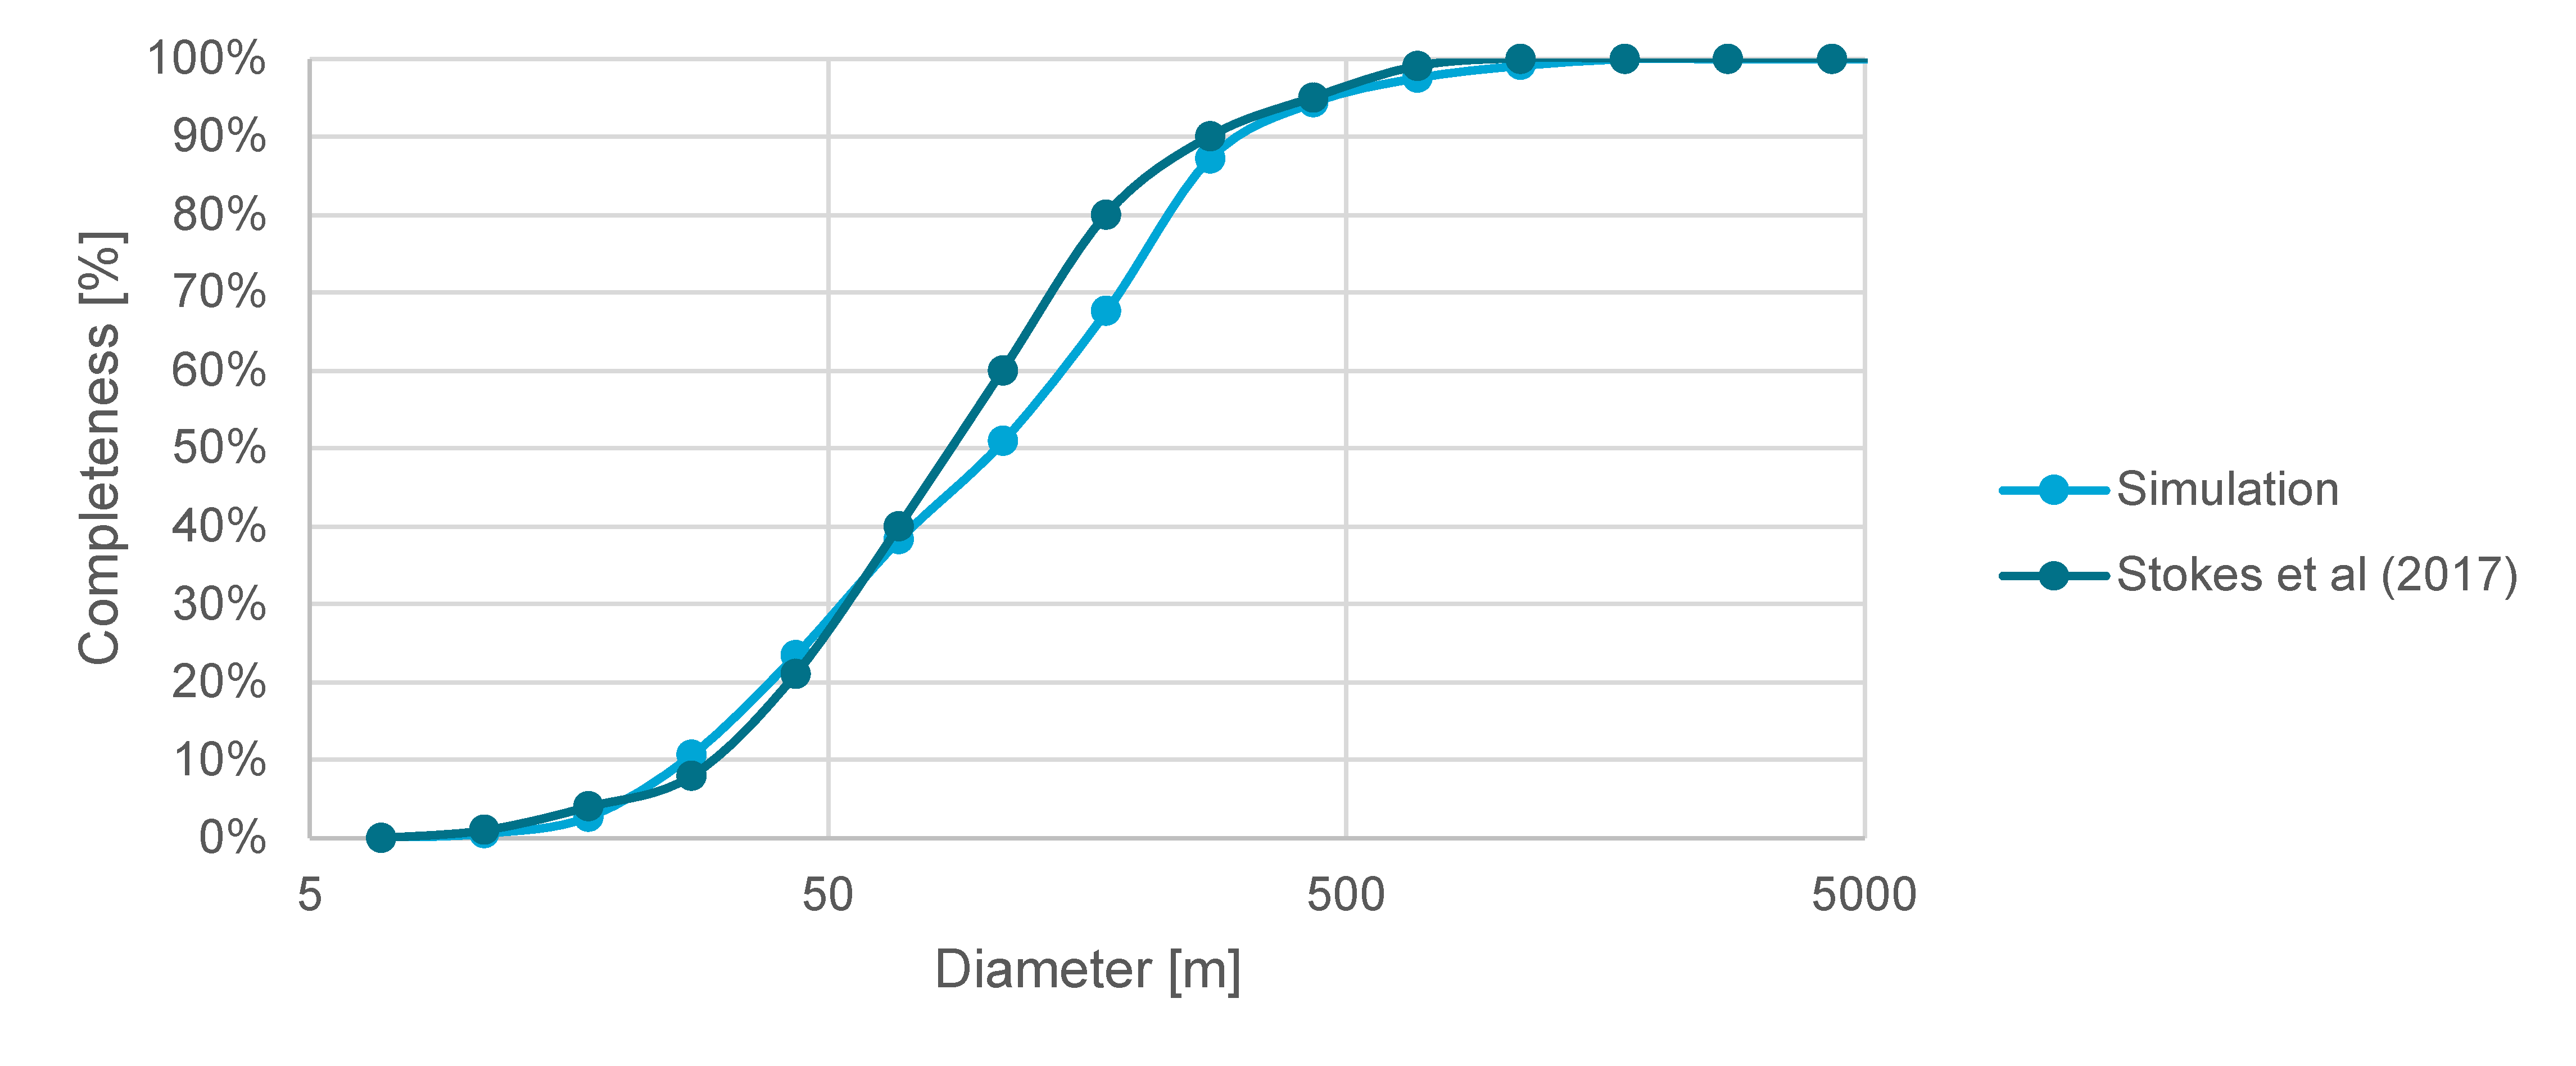
\includegraphics[width=0.8\textwidth]{img/validation_completeness_vis.pdf}
 \caption{Comparison of completeness as a function of diameter for visual light system, validation data from \cite{2017NEOSDT}.}
 \label{fig:validation_completeness_vis}
\end{figure}


\begin{figure}[htbp]
 \centering
 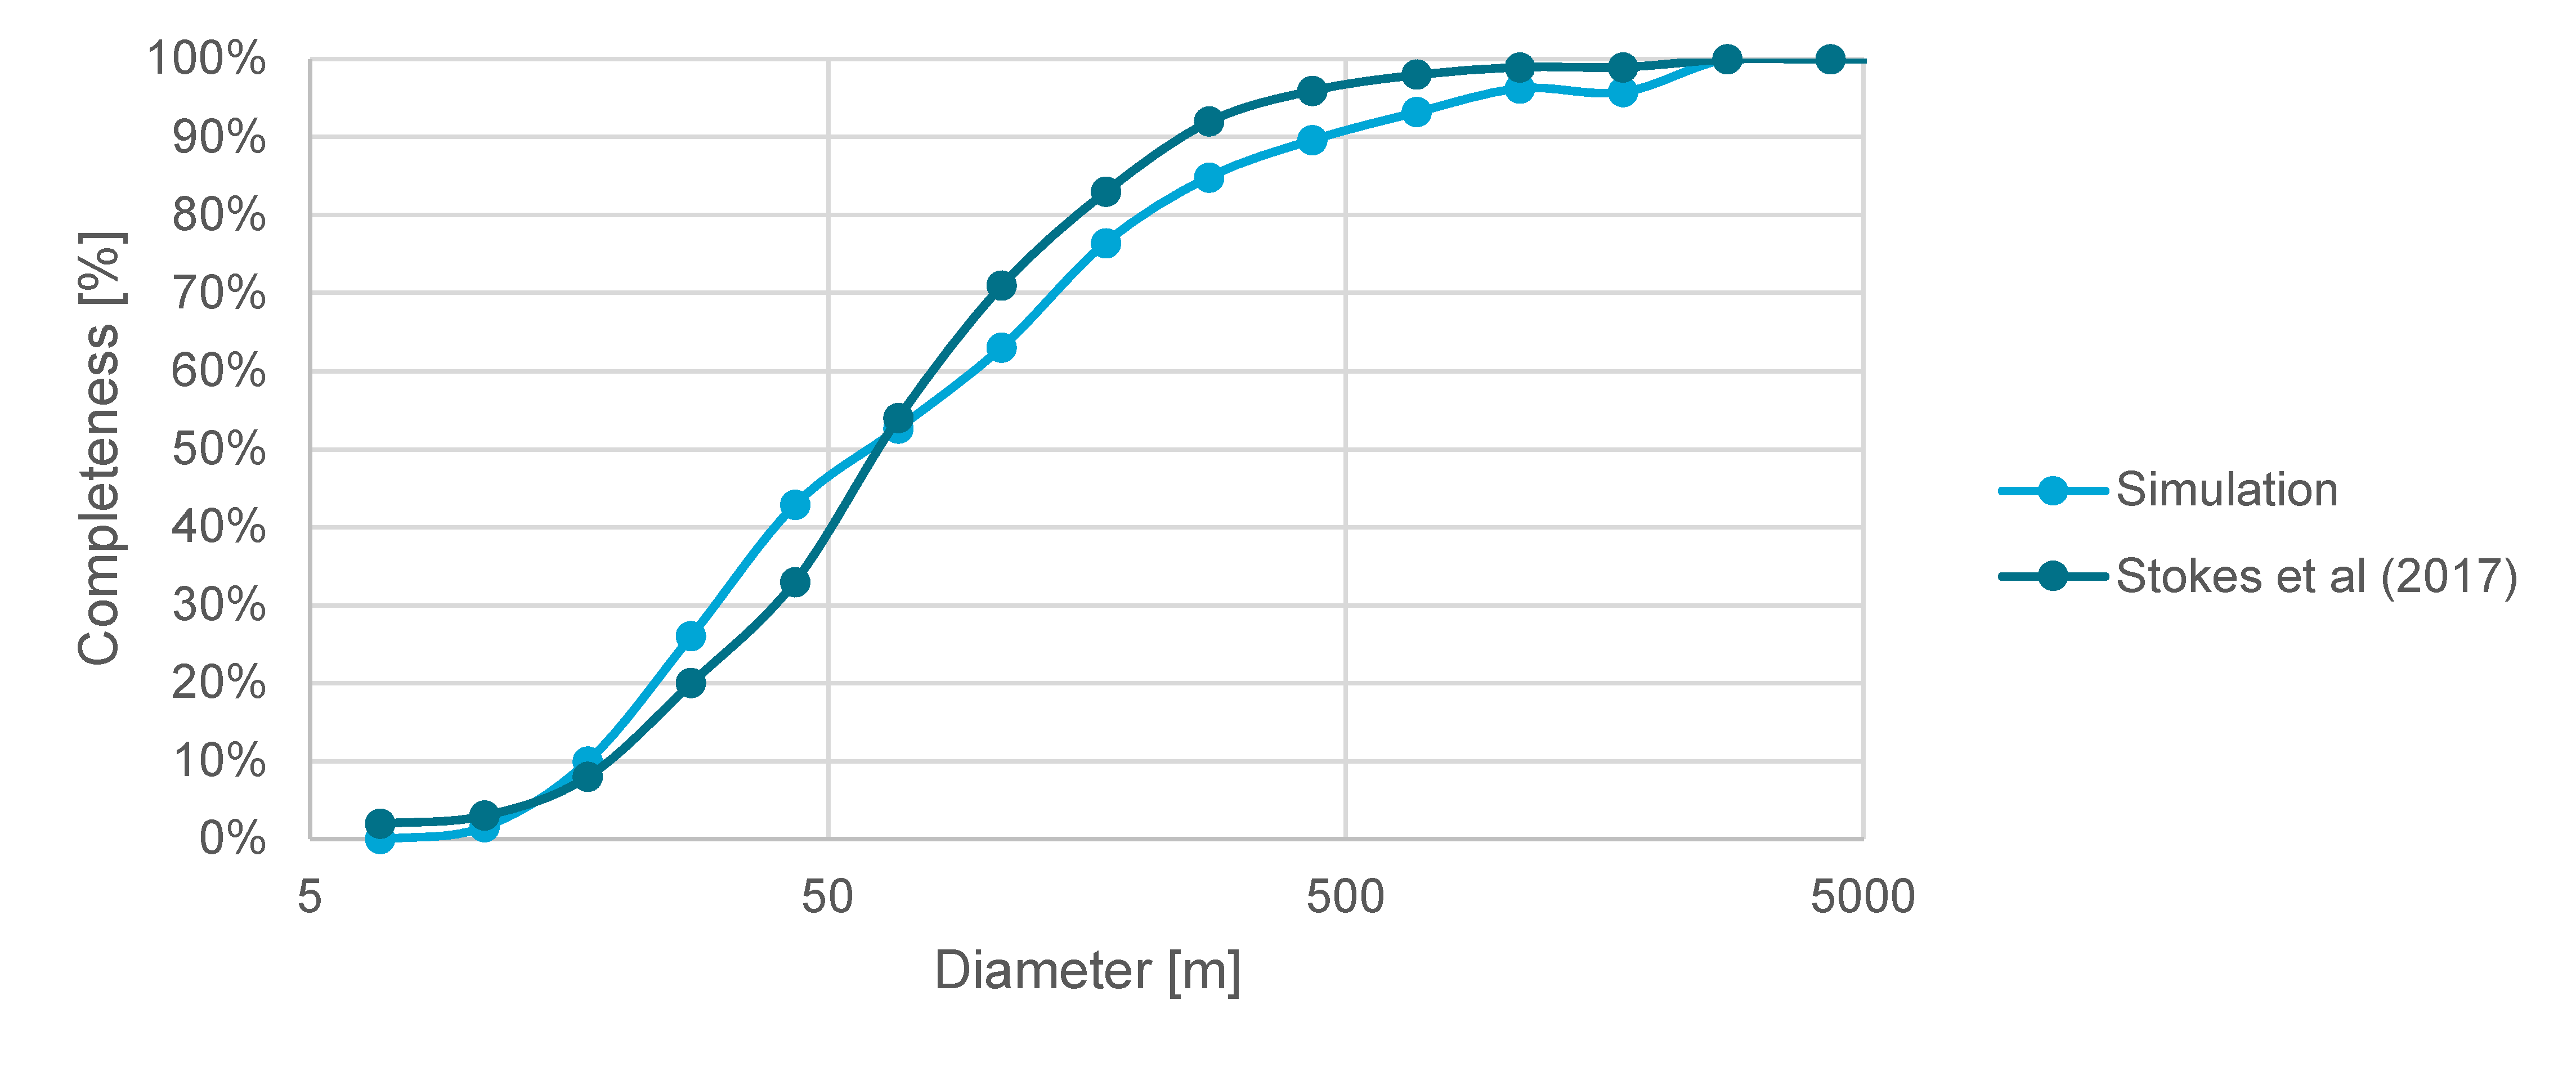
\includegraphics[width=0.8\textwidth]{img/validation_completeness_tir.pdf}
 \caption{Comparison of completeness as a function of diameter for thermal infrared system, validation data from \cite{2017NEOSDT}.}
 \label{fig:validation_completeness_tir}
\end{figure}

Results of the validation simulations are displayed in \autoref{fig:validation_completeness_vis} and \autoref{fig:validation_completeness_tir} for the visual light and thermal infrared payloads, respectively. Simulations were carried out using the same orbit and payload specifications as used in \cite{2017NEOSDT}. Results appear to be a good approximation. Some variation is however observed: The developed simulation predicts a lower performance for medium-sized asteroids of one to a few hundred meters in diameter, and a slightly higher performance for small-sized asteroids in the range of tens of meters. It is unknown what causes this deviation, although it is speculated that it might occur due to the function used to predict the results of \cite{2017NEOSDT}, as the curve shows almost no variance, whereas some variance would be expected. As the difference is small, and the overall completeness score differs by less than 1\% from the results of \cite{2017NEOSDT}, the simulation tool developed should give results that allow for accurate portrayal of reality, and accurate comparison to other studies and surveys.

\newpage
\chapter{Conclusion and Recommendations}
\label{ch:conclusion}
The aim of this report was to evaluate the possibilities and capabilities for surveying Near-Earth Asteroids using a system of multiple spacecraft. The main question to be answered was: ``What is the optimal position and composition for a system of spacecraft with the purpose of identifying and cataloguing previously unidentified Near-Earth Asteroids?''. To conclude the report, here the main question and associated subquestions will be answered, and conclusions will be drawn from these answers which can be used in the design of future NEA survey missions or future research into this topic. In addition, during research several opportunities were found for further research to better understand the capabilities of multi-spacecraft NEA surveys and to further develop the technology required to realise them. These opportunities will be turned into recommendations for future research.

\section{Conclusions}
Before summarizing the conclusions of the report, concrete answers to the research questions drafted in \autoref{sec:researchquestions} will be provided. Firstly, the various subquestions can be adressed:

\begin{enumerate}
 \item \textbf{How can the population of NEAs be accurately modelled, and how can these models be adjusted for unidentified NEAs?}: Modelling the population of NEAs was performed using a model created with the aid of NEOWISE data, compensated for biases in observation. This model was published by \cite{GranvikPopulation}, and is publicly available. As research focussed on still unidentified NEAs, the population was corrected with completeness statistics calculated from NEOWISE data by \cite{HarrisPopulation}. It should be noted that the accuracy of this approach is hard to verify; little data is available for comparison. However, comparison of the final performance to other models, even when considering the size-categories of asteroids, revealed no problems in the implementation of the population.
 \item \textbf{How can surveys of NEAs by a system of spacecraft be accurately modelled?}: Surveys were modelled by explicit calculation of the important steps in the process. First, the positions of all asteroids and spacecraft are calculated according to Keplerian orbits. Then, the background signal and target signals are calculated. From this, using representative hardware parameters, the signal-to-noise ratio can be obtained. Lastly, a probabilistic detection model is used to establish detection, and integration of the system in time allows for establishing identification. Components of the system were found from various sources in peer-reviewed literature, and their implementation was thoroughly verified and validated. In addition, it was shown that the simulation yielded similar results as other, previously validated survey models.
 \item \textbf{How can the position and composition of the system be optimized?}: The main challenge involved in optimizing the system is the fact that no useful analytical properties, such as gradients, are available, and the fact that the survey model is computationally expensive. For this reason, an approach of surrogate optimization was implemented. At lower numbers of spacecraft, the performance of this optimization method held up to results which were expected from initial data exploration. However, at higher numbers of spacecraft, and when considering more complicated optimization cases, the optimization method started to suffer problems related to overfitting. At this stage, the results of the optimization become unreliable, as it can be shown by direct comparison that it fails to obtain the optimal solution to the problem. It is therefore required to perform the more complicated optimizations using a more robust or powerful optimization algorithm in the future.
 \item \textbf{What is the effect of increasing the number of spacecraft on the process and performance of identifying and cataloguing NEAs?}: It was found that performance continuously increases with an increasing number of spacecraft. Initially, a second spacecraft yields very high improvements in performance - close to 50\% for thermal infrared systems - due to the possibility of performing triangulation, allowing for faster NEA identification. As the number of spacecraft further increases, the relative performance increase exponentially decreases. Therefore, systems with a large number of spacecraft will most likely not be cost-efficient compared to systems with less spacecraft, however addition of a second or third spacecraft will yield sizeable performance increases nonetheless.
 \item \textbf{How is the performance of possible payload compositions affected by the number of spacecraft, and what is the resulting optimal payload composition?}: It was shown that thermal infrared telescope payloads are the best choice for a future deep space NEA survey mission. Not only are thermal infrared telescopes superior to visual light telescopes for single spacecraft systems, the research presented in this report also shows that the relative performance increase of a thermal infrared system as the number of spacecraft is increased is higher than that of a visual light system. In addition, it was shown that for practical numbers of spacecraft, so-called hybrid systems with both visual light and thermal infrared telescopes did not provide enough synergistic benefits to outweight the worse performance of the visual light telescope.
 \item \textbf{How do the number of spacecraft and payload interact with the orbital parameters of the system?}: It was found that optimally, the spacecraft should be situated in a circular orbit, equally spaced out. The optimal semi-major axis of said orbit increases as the number of spacecraft increases, because else the spacecraft are placed closer together, introducing an inefficient overlap in their observation areas.
 \item \textbf{How effective is a system of multiple spacecraft at identifying and cataloguing previously unidentified NEAs compared to other current and future methods?}: A system of multiple spacecraft was shown to provide significant performance benefits to a single spacecraft system. Addition of a second spacecraft is expected to increase the improvement in completeness granted by a single spacecraft system by more than 50\% for asteroids in the tens to hundreds of meters in diameter. Further increases in the number of spacecraft will still yield improvements, however as the number of spacecraft increases, the majority of improvement will occur in the small, sub-100m diameter ranges. However, this approach has assumed that the spacecraft are capable of processing and transmitting the data indepently. Therefore, the ``cataloguing'' aspect remains an open area of research.
\end{enumerate}

After answering the subquestions, the main research question can be adressed: ``What is the optimal position and composition for a system of spacecraft with the purpose of identifying and cataloguing previously unidentified Near-Earth Asteroids?'' Through the research, it was found that the optimal NEA survey using multiple spacecraft should utilize the following:
\begin{itemize}
 \item \textbf{Number of spacecraft}: The number of spacecraft is dependent on the desired performance. It was shown that increasing the number of spacecraft will continue to increase the performance of the system, even when the system contains tens to hundreds of spacecraft. However, diminishing returns quickly set in and economic considerations should be included if an optimum is to be found.
 \item \textbf{Orbit}: The optimal orbit for the system was found to be a circular orbit, with the spacecraft spread out equally over the path of the orbit. In this way, the total volume of space effectively covered by the spacecraft is maximized, and does not vary in time.
 \item \textbf{Orbital radius}: The semi-major axis of the orbit should increase with increasing number of spacecraft, to reduce the overlap in spacecraft observation coverage as the distance between spacecraft reduces. Initially, for a single spacecraft, the optimum is found around 0.8 AU. For 2 or 3 spacecraft systems, the optimum lies around 1.0 AU. For a 4 to 5 spacecraft system, the optimal radius increases to around 1.1 AU. Further spacecraft will yield further increase of the semi-major axis. It was also found that the semi-major axis is not a very sensitive parameter for the performance, and deviation of up to 0.1 AU from the optimum will result in no statistically significant degradation of performance.
 \item \textbf{Payload}: Lastly, the system should be composed of spacecraft using telescopes built for imaging in the thermal infrared spectrum. As already shown by previous research, thermal infrared is preferred over visual light systems, as the background signal is weaker, leading to better signal-to-noise ratios for small targets. In addition, this research has shown that the relative benefit of using multiple spacecraft is greater when using thermal infrared telescopes. In addition, it is expected that thermal infrared sensor technology will still improve substantially in the coming years, adressing current shortcomings such as small sensor field-of-views and long integration times. This will improve the performance even further.
\end{itemize}

In conclusion, an analysis was provided of the behavior, ideal parameters, and expected performance of a multi-spacecraft NEA survey. Through answering the research question, a set of guidelines was obtained which can be used either directly in a design effort towards further surveying missions, or as a basis for future research. To facilitate in carrying out this research, the next section will provide some recommendations with regards to possible avenues to explore next.

\section{Recommendations for Further Research}
Throughout the research, several opportunities were identified to improve the understanding of multi-spacecraft NEA systems, or to further develop the necessary technologies. These form the basis of the recommendations listed below:
\begin{itemize}
 \item \textbf{NEA survey search strategies}: Currently, very little literature exists on the strategy that should be used for searching for NEAs. Although algorithms exist for single-spacecraft surveys, they are not extensively researched. In addition, no work has been done to exploit the possibilities of multi-spacecraft search strategies. For example, telescopes could focus their search effort in an area where another telescope has detected an NEA, or search strategies could be set up to maximize the occurence of triangulation, speeding up detection efforts significantly and helping to detect small, fast travelling NEAs.
 \item \textbf{On-board processing and communication limitations}: Throughout this report, it was assumed that spacecraft are capable of processing images from the telescopes and communicating within the system and to Earth. However, neither of these capabilities are currently proven (see \cite{LiteratureReview} for a full exploration). Therefore, work should be done on how a multi-spacecraft system can efficiently process and communicate the survey data.
 \item \textbf{Adressing the overfitting of the optimizer}: Detailed optimization efforts were hindered by a growing amount of overfit manifesting in the optimization efforts. As this thesis is not focussed on the topic of machine learning, and sufficient conclusions could be drawn, these results were left at that. However, to confirm the expectation that no significantly better solutions exists, it is suggested to attempt an optimization method which is less susceptible to noise in the signal. The recommendation would be to first attempt a different surrogate model, such as using an artificial neural network, instead of a classical machine learning approach, and possibly branching our further from that.
 \item \textbf{Investigation of the problem in non-Keplerian celestial mechanics}: Although the error in the solution is expected to be small, it is recommended to validate this by performing a three-body or n-body simulation of the problem. This might also interplay with advances in the search strategies, as more subtleties in the orbits of NEAs become important for the performance. In addition, non-Keplerian mechanics might allow exploitation of different orbital configurations for the system of spacecraft. In particular, utilization of Lagrange point could allow for implementation of differing semi-major axes per spacecraft, whilst still maintaining a constant distance between the spacecraft throughout their mission.
\end{itemize}

\newpage

%% Use letters for the chapter numbers of the appendices.
\appendix

\chapter{Optimization Results}
\label{ch:appendix}

\textit{This page was intentionally left blank so the orbits and learning curves can be viewed side-by-side in print}

\begin{figure}[p]
 \centering
 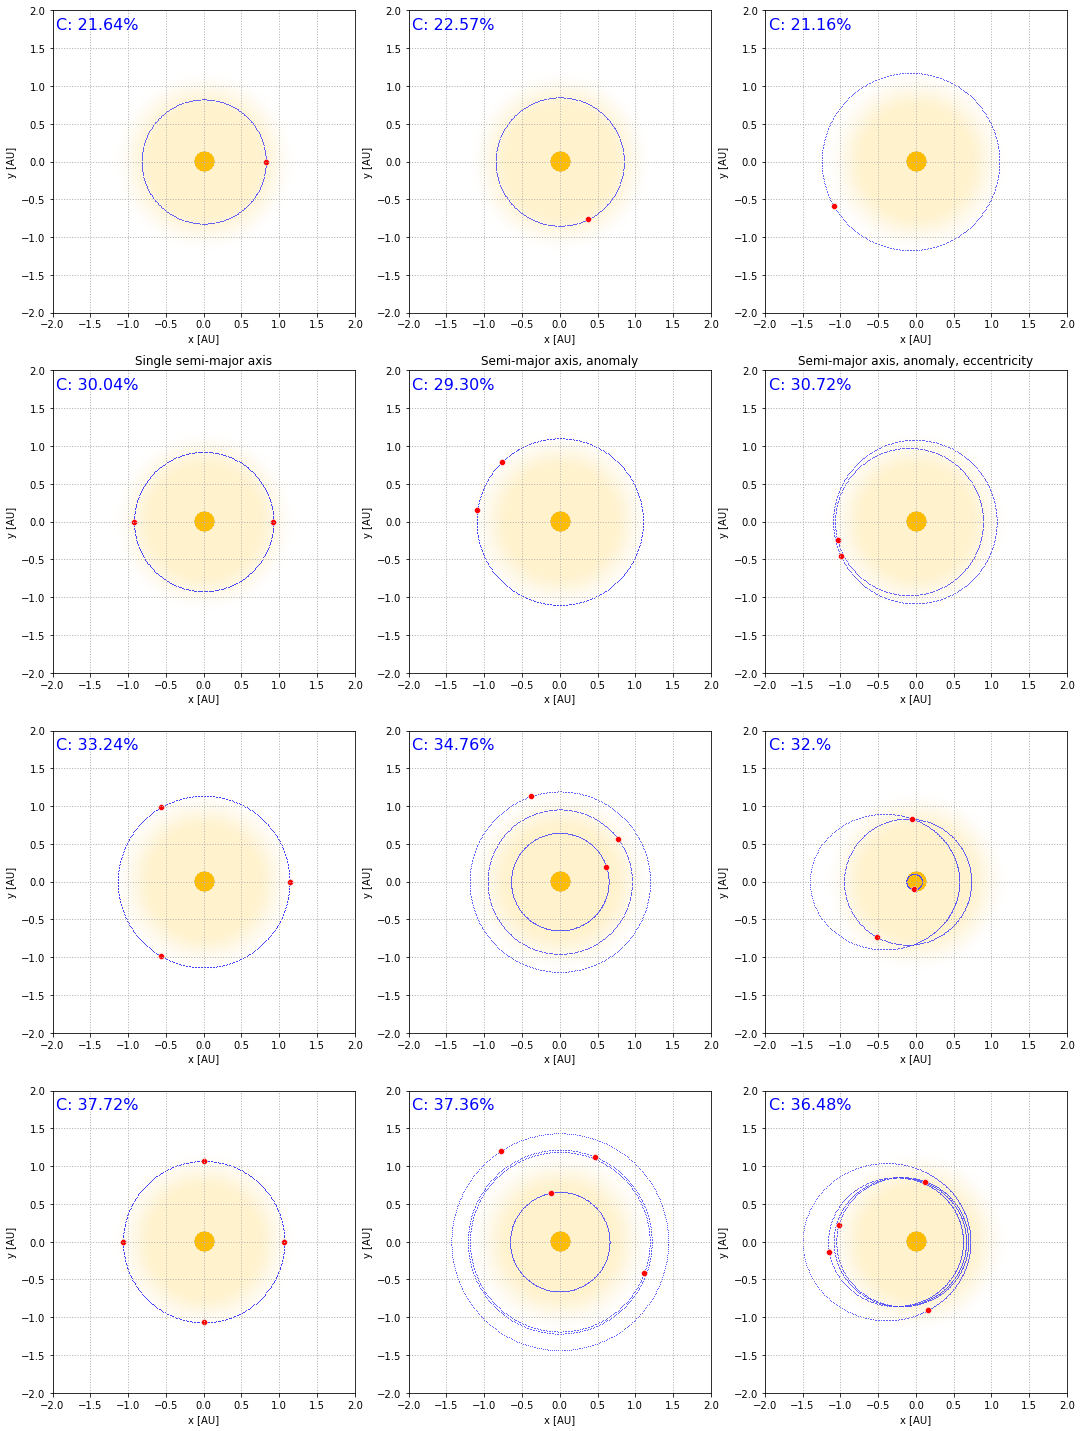
\includegraphics[width=1.0\textwidth]{img/appendix_orbit_1.png}
 \caption{Optimization solutions for 1-4 spacecraft. Left: circular co-orbital, middle: individual semi-major axis and anomaly, right: individual semi-major axis, anomaly and eccentricity.}
\end{figure}

\begin{figure}[p]
 \centering
 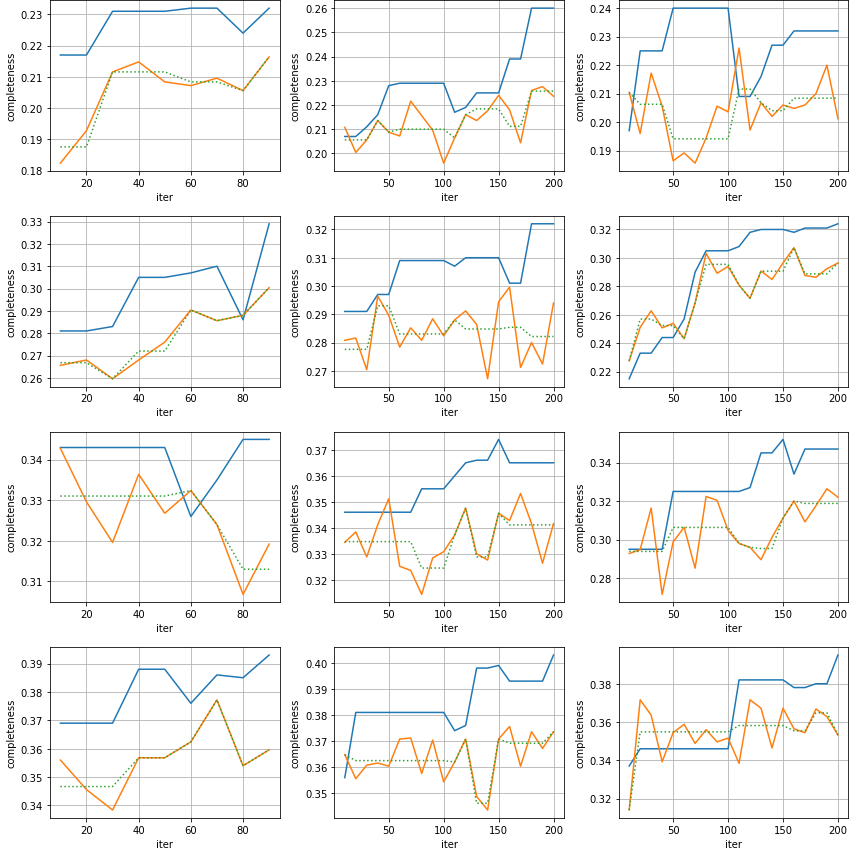
\includegraphics[width=1.0\textwidth]{img/appendix_loss_1.png}
 \caption{Learning and loss curves for optimization of 1-4 spacecraft. Blue line: learning, orange line: validation, green dotted line: average of validation for a given solution.}
\end{figure}



\begin{figure}[p]
 \centering
 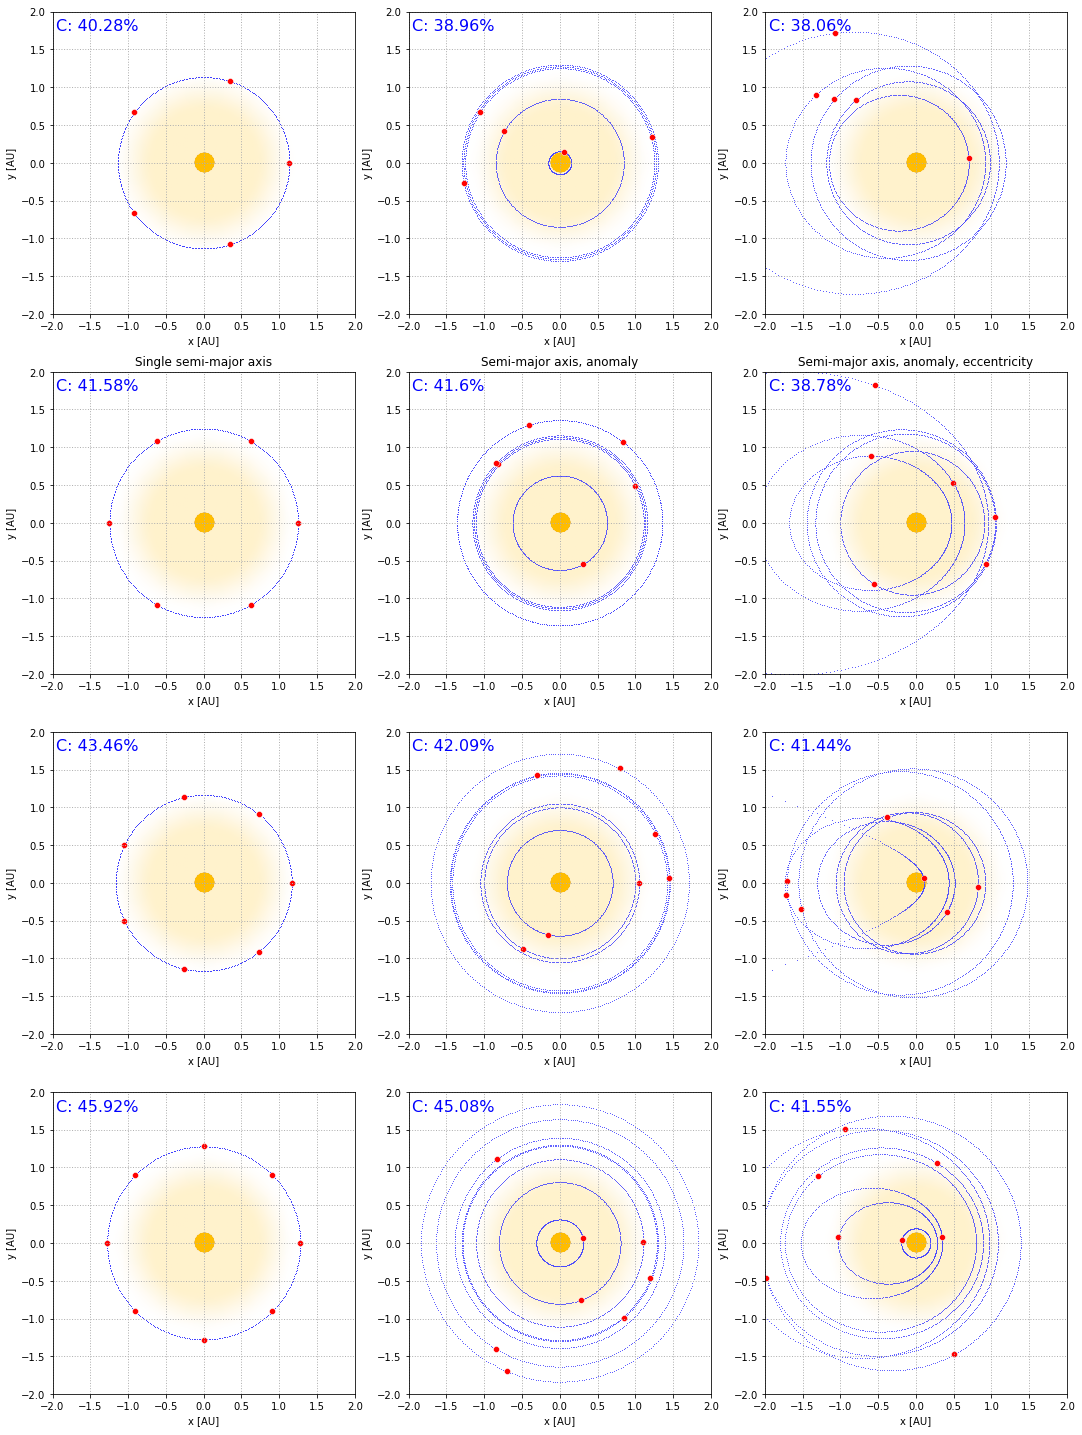
\includegraphics[width=1.0\textwidth]{img/appendix_orbit_2.png}
 \caption{Optimization solutions for 5-8 spacecraft. Left: circular co-orbital, middle: individual semi-major axis and anomaly, right: individual semi-major axis, anomaly and eccentricity.}
\end{figure}

\begin{figure}[p]
 \centering
 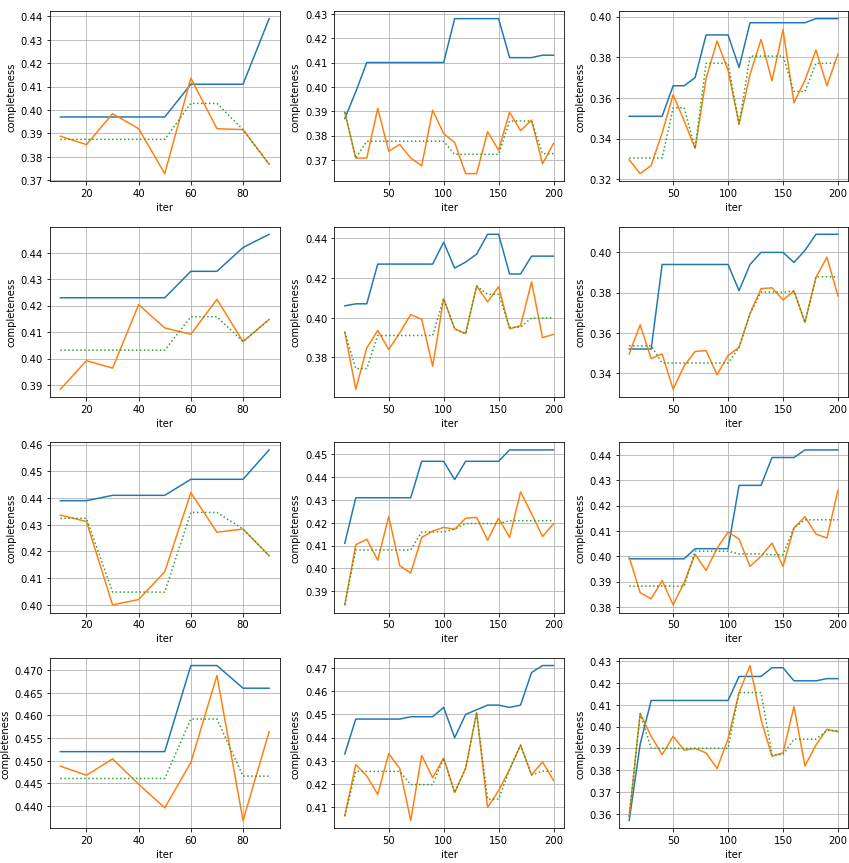
\includegraphics[width=1.0\textwidth]{img/appendix_loss_2.png}
 \caption{Learning and loss curves for optimization of 5-8 spacecraft. Blue line: learning, orange line: validation, green dotted line: average of validation for a given solution.}
\end{figure}



\begin{figure}[p]
 \centering
 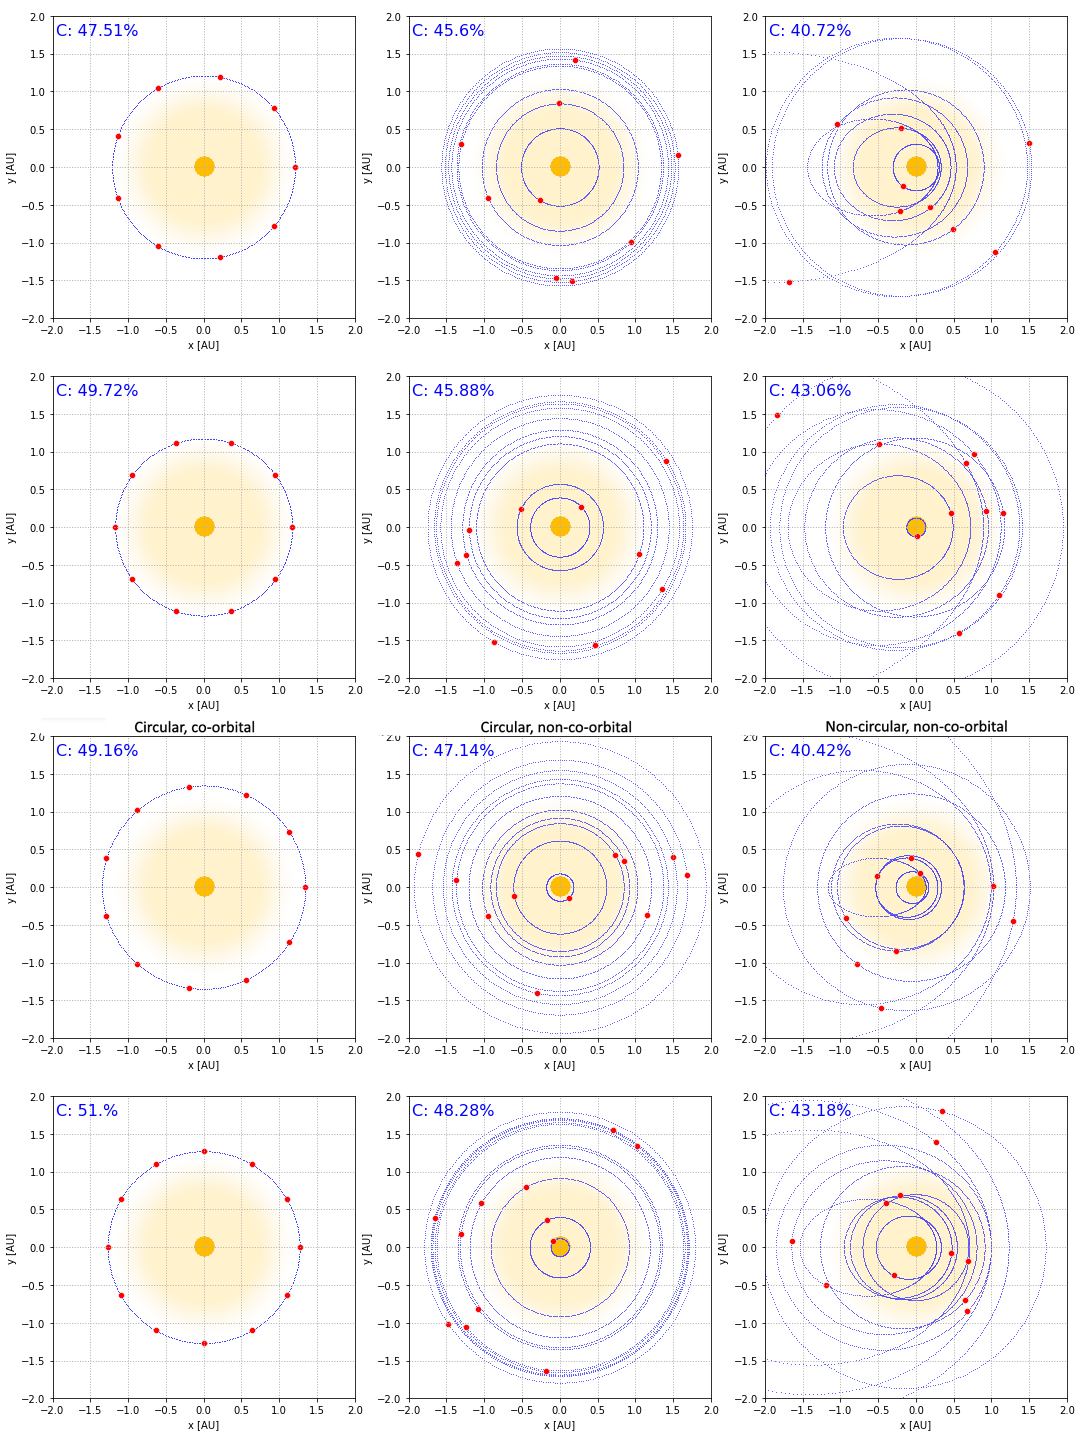
\includegraphics[width=1.0\textwidth]{img/appendix_orbit_3.png}
 \caption{Optimization solutions for 9-12 spacecraft. Left: circular co-orbital, middle: individual semi-major axis and anomaly, right: individual semi-major axis, anomaly and eccentricity.}
\end{figure}

\begin{figure}[p]
 \centering
 \includegraphics[width=1.0\textwidth]{img/appendix_loss_3.png}
 \caption{Learning and loss curves for optimization of 9-12 spacecraft. Blue line: learning, orange line: validation, green dotted line: average of validation for a given solution.}
\end{figure}



\begin{figure}[p]
 \centering
 \includegraphics[width=1.0\textwidth]{img/appendix_orbit_4.png}
 \caption{Optimization solutions for 13-16 spacecraft. Left: circular co-orbital, middle: individual semi-major axis and anomaly, right: individual semi-major axis, anomaly and eccentricity.}
\end{figure}

\begin{figure}[p]
 \centering
 \includegraphics[width=1.0\textwidth]{img/appendix_loss_4.png}
 \caption{Learning and loss curves for optimization of 13-16 spacecraft. Blue line: learning, orange line: validation, green dotted line: average of validation for a given solution.}
\end{figure}



\begin{figure}[p]
 \centering
 \includegraphics[width=1.0\textwidth]{img/appendix_orbit_5.png}
 \caption{Optimization solutions for 17-20 spacecraft. Left: circular co-orbital, middle: individual semi-major axis and anomaly, right: individual semi-major axis, anomaly and eccentricity.}
\end{figure}

\begin{figure}[p]
 \centering
 \includegraphics[width=1.0\textwidth]{img/appendix_loss_5.png}
 \caption{Learning and loss curves for optimization of 17-20 spacecraft. Blue line: learning, orange line: validation, green dotted line: average of validation for a given solution.}
\end{figure}


\printbibliography

\end{document}

